\documentclass[12pt,a4paper,twoside]{NITR}

\usepackage[hyphens]{url} 
%\usepackage[usenames,dvipsnames]{color}
%\usepackage[colorlinks=true,breaklinks,backref=true,linkcolor={MidnightBlue},citecolor={Fuchsia},urlcolor={OliveGreen}]{hyperref}
\usepackage[none]{hyphenat}
\usepackage{amsmath,amsfonts,mathdots,amssymb,yfonts}
\usepackage{graphicx}
\usepackage{tikz}
\usepackage{subfigure}
\usetikzlibrary{trees,shapes}
\usepackage{booktabs}
\usepackage{textgreek}
\usepackage[a4paper, width=140mm, top=25mm, bottom=25mm, bindingoffset=6mm]{geometry}
\usepackage{layaureo}
% \usepackage[square, numbers, comma, sort&compress]{natbib}
\usepackage{adjustbox}
\usepackage{blindtext}
% \ifCLASSINFOpdf
% \usepackage[pdftex]{graphicx}
\usepackage{amsmath}
\usepackage{csquotes}
\usepackage{array}
% \usepackage{tabu}
\usepackage[caption=false]{subfig}
\usepackage{lipsum}
\usepackage{caption}
% \usepackage{subcaption}
\usepackage{todonotes}
% \usepackage{subfig}
\usepackage[utf8]{inputenc}
\usepackage[T1]{fontenc}  
\usepackage{multirow}
\usepackage{makecell}
\usepackage{ctable} %For special rule
\usepackage{float}
\usepackage{rotating}

\usepackage{hyperref}
% \usepackage[demo]{graphicx}
% \usepackage{subfig}
% % % % % % % % % % % % % % % % % % % % % % % % % % %
% % % % % % % % % % % % % % % % % % % % % % % % % % %
% \usepackage{mmap}
% \usepackage{lmodren}
% \usepackage[utf8]{inputenc}
% \usepackage[french]{babel}
\usepackage{listings}
\usepackage{xcolor}

\definecolor{codegreen}{rgb}{0,0.6,0}
\definecolor{codegray}{rgb}{0.5,0.5,0.5}
\definecolor{codepurple}{rgb}{0.58,0,0.82}
\definecolor{backcolour}{rgb}{0.95,0.95,0.92}

\lstdefinestyle{mystyle}{
    backgroundcolor=\color{backcolour},   
    commentstyle=\color{codegreen},
    keywordstyle=\color{magenta},
    numberstyle=\tiny\color{codegray},
    stringstyle=\color{codepurple},
    basicstyle=\ttfamily\footnotesize,
    breakatwhitespace=false,         
    breaklines=true,                 
    captionpos=b,                    
    keepspaces=true,                 
    numbers=left,                    
    numbersep=5pt,                  
    showspaces=false,                
    showstringspaces=false,
    showtabs=false,                  
    tabsize=2
}

\lstset{style=mystyle}
% % % % % % % % % % % % % % % % % % % % % % % % % % %
% % % % % % % % % % % % % % % % % % % % % % % % % % %




   \makeatletter
\newcommand{\thickhline}{%
    \noalign {\ifnum 0=`}\fi \hrule height 1pt
    \futurelet \reserved@a \@xhline
}
\usepackage[firstpage=true]{background}
% \usepackage[pages=some]{background}
\backgroundsetup{
scale=1,
firstpage=true,
color=black,
opacity=0.05,
angle=0,
contents={%
  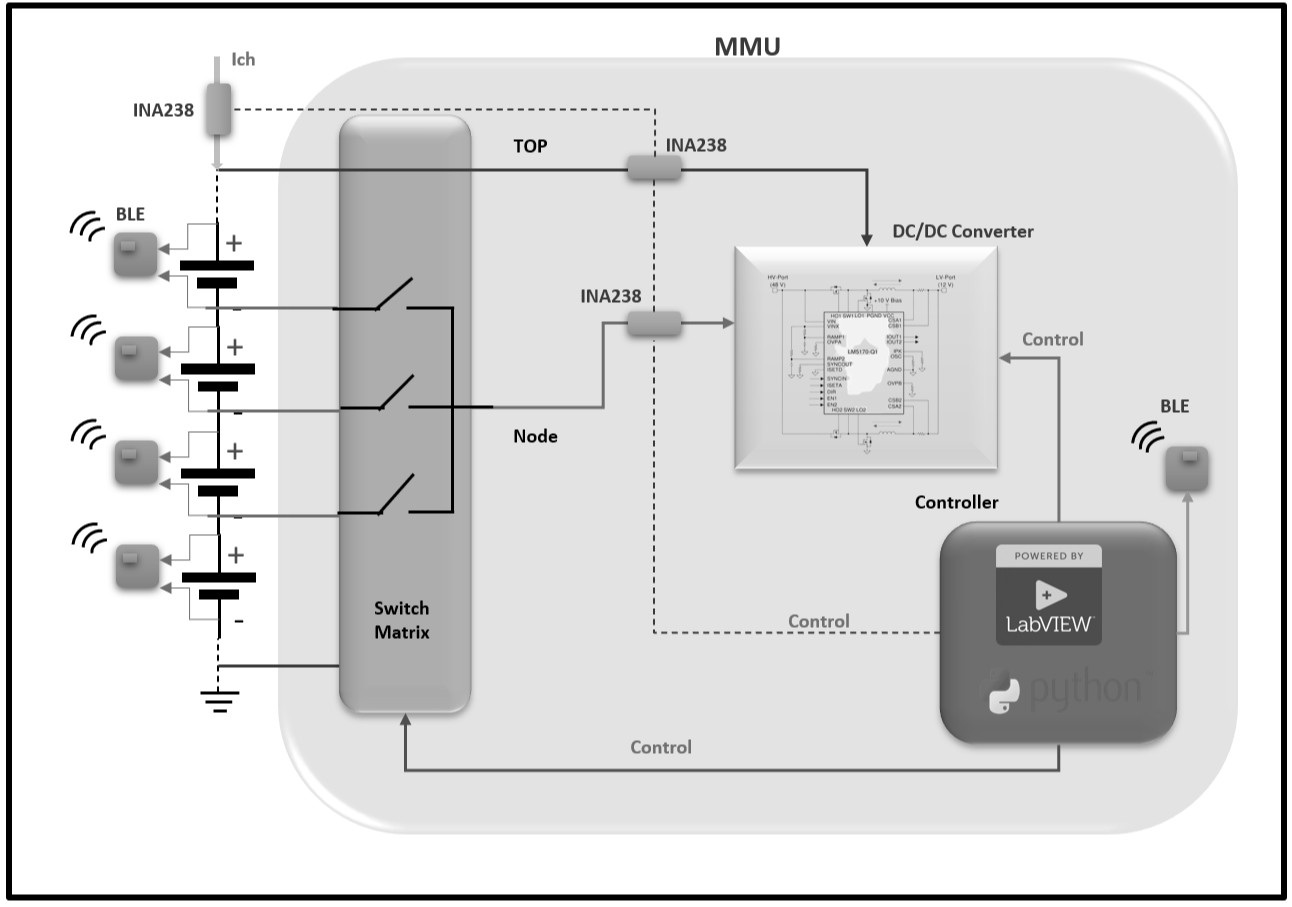
\includegraphics[width=0.8\paperwidth]{BMS_Architecture_border-modified.PNG}
  }%
}
\renewcommand{\thesubsubsection}{\thesubsection.\alph{subsubsection}}
\setcounter{secnumdepth}{4}

%\usepackage{subfigure}
%\usepackage[ruled,linesnumbered,slide,vlined]{algorithm2e}
%\usepackage{verbatim}
%\usepackage{wrapfig}
%\usepackage{multirow}


%% % % % % % %
\onehalfspacing
\begin{document}
\sloppy
% % % % % % % % % % % % % % % % % % % % % % % % % % %
% % % % % % % % % % % % % % % % % % % % % % % % % % %
\author{Harish Kumar Shivaramappa}

\authorGender{male}		
\department{Department of Electrical, Computer and Biomedical Engineering}
\docTitle{SOC and SOH estimation in BMS based on Wireless Communication Network}

% % % % % % % % % % % % % % % % % % % % % % % % % % % % % %
% % % % % % % % % % % % % % % % % % % % % % % % % % % % % %
% % %
\studentType{Master}			

	
% % % % % % % % % % % % % % % % % % % % % % % % % % % % % %
% % % 


\degree{Master of Science} 				     %%Master of Science; 


% % % % % % % % % % % % % % % % % % % % % % % % % % % % % %
% % % % % % % % % % % % % % % % % % % % % % % % % % % % % %

% % % Mention the discipline in which the degree is awarded
\degreeIn{Microelectronics}		


% % % % % % % % % % % % % % % % % % % % % % % % % % % % % %
% % % % % % % % % % % % % % % % % % % % % % % % % % % % % %

\docType{1}		%%Dissertation=1; Thesis=2; Project=3; Synopsis=4; Registration Report=5

% % % % % % % % % % % % % % % % % % % % % % % % % % % % % %
% % % % % % % % % % % % % % % % % % % % % % % % % % % % % %

\numOfSupervisors{2}

\principalSupervisor{Piero Malcovati}	%%Name only
\coSupervisor{Domenico Granozio}			%%Name only
\principalSupervisorDesignation{Professor}
% \coSupervisorDesignation{Eng}

% % % % % % % % % % % % % % % % % % % % % % % % % % % % % %
% % % % % % % % % % % % % % % % % % % % % % % % % % % % % %

% Just for the Sample Date 
\setDate{20}
\setMonth{December}
\setYear{2022}

% % % % % % % % % % % % % % % % % % % % % % % % % % % % % %
% % % % % % % % % % % % % % % % % % % % % % % % % % % % % %

\Font{1}	%% Times New Roman=1; Arial=2;
\setFont

% % % % % % % % % % % % % % % % % % % % % % % % % % % % % %
% % % % % % % % % % % % % % % % % % % % % % % % % % % % % %
% % % 

\titlePageLineSpacing{2}
\titleWidth{.75}
\titleCoordinateX{0.13}
\titleCoordinateY{0.12}

% % % % % % % % % % % % % % % % % % % % % % % % % % %
% % % % % % % % % % % % % % % % % % % % % % % % % % %
% % % % % % % % % % % % % % % % % % % % % % % % % % %
	% %Fill details in "FrontPages.tex"
% % % % % % % % % % % % % % % % % % % % % % % % % % %
% % % % % % % % % % % % % % % % % % % % % % % % % % %
%%\coverPageSynReg		% %Needed for Synopsis Cover Page or 
						% %Registration Report Cover Page.
						% %To be used along with "\docType()".
						% %Use "\section{Introduction}\label{Guidelines}
Submission of a synopsis or extended abstract is one of the mandatory requirements before submitting a doctoral or master thesis. It is not just a longer version of an abstract. It is as good as a research paper that conveys the essence of the thesis without overlooking the importance of introduction and conclusion. A synopsis should include the following~\textemdash~
\begin{itemize}
	\item Introduction
	\item Aim
	\item Method
	\item Results
	\item Conclusion
	\item Limitations
	\item References
	\item Dissemination
\end{itemize}

\noindent A synopsis is a self-contained, capsule description of the thesis that must make sense all by itself. Typical length of a synopsis should be between 5 and 10. Pages must of A4 dimension with 25mm margin on all four sides. The entire dissertation must be written using only a single font including all the texts inside graphs, figures, block diagrams, etc. While writing captions of tables and figures, the font size should be decreased by one point. Similarly, the font size of bibliography and index should also be lessened by a point. Students are advised to use the following in the body text~\textemdash
\begin{itemize}
\item[] serif fonts like Times New Roman (TNR) of size 12pt \\
or \\
\textsf{sans-serif fonts like Arial of size 11pt}. 
\end{itemize}
Needless to say that the use of font should be uniform throughout. Headings, Titles \textit{etc.} should use fonts as given below in Table~\ref{tab-fonts}.
{
\linespread{1}
\begin{table}[h]
\centering
\caption{Font sizes to be used in the dissertation}
\begin{tabular}{l C{25mm} C{25mm} c} 
\toprule
{Item} & Arial & {TNR} & {Justification}\\
\midrule\midrule
Main Text & 11 normal & 12 normal & Justified \\
\midrule
Sub-sub Heading & 11 bold & 12 bold & Left \\
\midrule
Sub Heading & 13 bold & 14 bold & Left \\
\midrule
Heading$^{\#}$ & 16 bold & 17 bold & Left \\
\midrule
Chapter Title & 22 bold & 24 bold & Center \\
\midrule
Chapter Number & 16 bold & 17 bold & Left \\
\bottomrule
\multicolumn{4}{l}{$^{\#}$Add serial number with one decimal place.} 
\end{tabular}
\label{tab-fonts}
\end{table}
}
\par The class file \texttt{NITR.cls} can be used to prepare a synopsis. One needs to invoke the statement ``\texttt{\textbackslash synopsisCoverPage}'' in the main ``\texttt{.tex}'' file with ``\texttt{\textbackslash docType(4)}'' and all necessary data in the ``\texttt{FrontPages.tex}''. The text of the synopsis can be written in ``\texttt{./SynopsisText/SynopsisText.tex}''."
						% %Comment rest.
\coverPage
\titlePage
% \certificateOfExamination

%\certificateOneSupervisor		%% Comment any
% \certificateTwoSupervisors		%% one of these two

\dedication
% \declaration

\acknowledgment
\abstract
% % % % % % % % % % % % % % % % % % % % % % % % % % %
% % % % % % % % % % % % % % % % % % % % % % % % % % %
% \chapter{Preface}
When started my Microelectronics master's program at the University of Pavia, I was wondering about the future of microelectronics in the domain of electric vehicle and sustainable energy management because I have witnessed personally how world leaders are crumbling to fix global warming and climate change. The idea of making global warming free through sustainable energy drove me to explore electrical vehicles and power management. As I was intensively researching my self about electrical vehicles and battery management systems, I got an opportunity to enroll LM+ program at the university of Pavia which is doing an internship through the university in corporate companies for one year.\\
\indent Among the LM+ opportunities, I have noticed that Inventvm a dynamic young Italian company is doing research on Battery management systems for electrical vehicles. Since my interest is to work in power management and sustainable energy management, the Inventvm BMS project became a cherry on the pie for me. During the process, I met Eng. Domenico (Inventvm project BMS project manager), his idea of an elaboration made me more curious about the project and I stretched my legs immediately to the Inventvm on Feb 2020.\\
\indent As I was stepping into Inventvm I started to experience the radiation of the knowledge from the engineers because they are not kids like me. As a young rookie in technology, I start to learn more about the hardware and software of the project because the bus(project) is already started way before I join to the company. That was ok! because at the age of 10 I smoked the LED placing it in 230V mains, what ??????? YES that's right, for sure the led did not glow bright, but my brain became to dig into why LED got burned despite the black smoke on the face while LED burned. Anyway, later I was educated by my father(of course he is an electrician) that LED needs some kind of electronic circuit to make it glow. when my father made LED glow, That was WoW, "astonishing"! LED was not too much bright enough though. This idea of making education by failure became fascinating this same strategy worked for me to understand this in the industry too quickly not to miss the bus. There are always my colleagues who gave me a shoulder to shoulder when I was stuck in some technological part.\\
\indentBefore my Master's, I worked with Analog Device Inc as IoT application Engineer and System Testing Engineer for Highpower circuits In NEXTGEN computers helped in my current project to understand the Wireless communication environment and power management. My experience in these two prime companies laid the foundation for analytical skills and problem-picking skills throughout the project. Nevertheless, the key motivation was my father and all my teachers who educated me throughout my life to contribute well to nature and humanity. Nonetheless, Prof malcovati has been a gem among all my honorable teacher's treasury who shined bright in my way. Thanks......!
% \thispagestyle{empty}
% \cleardoublepage
% % % % % % % % % % % % % % % % % % % % % % % % % % %
% % % % % % % % % % % % % % % % % % % % % % % % % % %
\tableofcontents
\cleardoublepage
% % % % % % % % % % % % % % % % % % % % % % % % % % %
% % % % % % % % % % % % % % % % % % % % % % % % % % %
\addcontentsline{toc}{chapter}{List of Figures}
\listoffigures
\cleardoublepage
% % % % % % % % % % % % % % % % %
\addcontentsline{toc}{chapter}{List of Tables}
\listoftables
\cleardoublepage
% % % % % % % % % % % % % % % % % % % % % % % % % % %
% % % % % % % % % % % % % % % % % % % % % % % % % % %
\pagenumbering{arabic}
\pagestyle{fancy}
\renewcommand{\chaptermark}[1]{\markboth{#1}{}}
\renewcommand{\sectionmark}[1]{\markright{\textbf{Chapter \thechapter}}}

% % % % % % % % % % % % % % % % % % % % % % % % % % %
% % % % % % % % % % % % % % % % % % % % % % % % % % %
\chapter{Preface}
When started my Microelectronics master's program at the University of Pavia, I was wondering about the future of microelectronics in the domain of electric vehicle and sustainable energy management because I have witnessed personally how world leaders are crumbling to fix global warming and climate change. The idea of making global warming free through sustainable energy drove me to explore electrical vehicles and power management. As I was intensively researching my self about electrical vehicles and battery management systems, I got an opportunity to enroll LM+ program at the university of Pavia which is doing an internship through the university in corporate companies for one year.\\
\indent Among the LM+ opportunities, I have noticed that Inventvm a dynamic young Italian company is doing research on Battery management systems for electrical vehicles. Since my interest is to work in power management and sustainable energy management, the Inventvm BMS project became a cherry on the pie for me. During the process, I met Eng. Domenico (Inventvm project BMS project manager), his idea of an elaboration made me more curious about the project and I stretched my legs immediately to the Inventvm on Feb 2020.\\
\indent As I was stepping into Inventvm I started to experience the radiation of the knowledge from the engineers because they are not kids like me. As a young rookie in technology, I start to learn more about the hardware and software of the project because the bus(project) is already started way before I join to the company. That was ok! because at the age of 10 I smoked the LED placing it in 230V mains, what ??????? YES that's right, for sure the led did not glow bright, but my brain became to dig into why LED got burned despite the black smoke on the face while LED burned. Anyway, later I was educated by my father(of course he is an electrician) that LED needs some kind of electronic circuit to make it glow. when my father made LED glow, That was WoW, "astonishing"! LED was not too much bright enough though. This idea of making education by failure became fascinating this same strategy worked for me to understand this in the industry too quickly not to miss the bus. There are always my colleagues who gave me a shoulder to shoulder when I was stuck in some technological part.\\
\indentBefore my Master's, I worked with Analog Device Inc as IoT application Engineer and System Testing Engineer for Highpower circuits In NEXTGEN computers helped in my current project to understand the Wireless communication environment and power management. My experience in these two prime companies laid the foundation for analytical skills and problem-picking skills throughout the project. Nevertheless, the key motivation was my father and all my teachers who educated me throughout my life to contribute well to nature and humanity. Nonetheless, Prof malcovati has been a gem among all my honorable teacher's treasury who shined bright in my way. Thanks......!
\thispagestyle{empty}
\cleardoublepage
% % % % % % % % % % % % % % % % % % % % % % % % % % %
% % % % % % % % % % % % % % % % % % % % % % % % % % %
%Formatting Guidelines for Writing Dissertation.
\chapter{Introduction}\label{intro}

\ \ \ \ \ \ \  
\thispagestyle{empty}
\cleardoublepage
% % % % % % % % % % % % % % % % % % % % % % % % % % %
% % % % % % % % % % % % % % % % % % % % % % % % % % %
% %Some Unstructured Advice on Dissertation Writing
\chapter{Literature Survey}\label{literature_survey}

Sigma-Delta Modulators find a variety of applications such as consumer electronics, automotive applications, sensor read-out applications, environmental measurements, medical instrumentation, military applications etc. 



A continuous time baseband {\textSigma}{\textDelta}M \cite{breems20001} was implemented for the A/D conversion for the intermediate frequency (IF) signals.

\cite{breems20001} \cite{fujimori200090} \cite{morizio200014} \cite{rosa2000cmos}


% \thispagestyle{empty}
% \cleardoublepage
% % % % % % % % % % % % % % % % % % % % % % % % % % %
% % % % % % % % % % % % % % % % % % % % % % % % % % %

\chapter{Bluetooth Module Design}\label{chap:BLE}
% \stepcounter{chapter}\addcontentsline{toc}{chapter}{Incremental Sigma-Delta Modulator}

\section{Introduction}


Antenna design and analysis are crucial in a wireless network that transmits and receives information through electromagnetic wave radiation in open space.
Modern Antenna and RF design techniques are more often testified against size, power, flexibility, radiation patterns, efficiency, etc...
It is very unusual to use a wide variety of RF fundamental design techniques even though the usage of silicon and power is different because the fundamentals of RF design are most rigorous and robust from decades, hence RF fundamentals and design techniques remain intact. Nevertheless, modern RF applications demand to emphasize efficiency and power requirements, so this requirement needs some special RF Design treatments.
Chapter .3 gives the extravagance of PCB antenna design practices, general guidelines for grounding, PCB stacking, spacings and via holes, etc. Matching networks in RF design are extremely important to increase the efficiency of the Antenna and RF line, so it is also explored in the same chapter how to pick the passive components for RF Antenna matching such as capacitors and inductors.

%%%%%%*********************************************************%%%%%%%
%%%%%%*************************New Section*********************%%%%%%%
%%%%%%*********************************************************%%%%%%%
\section{Antenna Basics :}

An Antenna is a piece of metal exposed to free space. A piece of conductor behaves like an antenna when its length is a certain ratio or multiple of the wavelength of the signal. This scenario is expressed as "resonance", where the antenna radiates the electrical energy to the open space.




\begin{figure}[h]
	\centering
	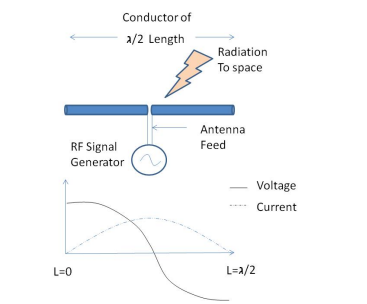
\includegraphics[width=0.7\textwidth]{Chap03/Figures/Basic_Antenna.PNG}
	\caption{Basic dipole Antenna}
	\label{BASIC_ANTENNA}
\end{figure}

Fig.1  shows the dipole antenna whose length is  $\lambda/2$ and the fed has an input impedance of $50\Omega $.
Dipole antennas are the most basic antennas that have been used for broadcasting.
In the Millennial age of technology, dipole antennas have been bulky and heavy, thanks to the PCB technology, which made dipole antennas extremely simple in construction and this became the center of attraction for the Bluetooth application in the modern era.
Although dipole antennas are extremely comfortable for PCB we still face hurdles to manage proper grounding for the antenna..which can be addressed through quarter-wave antennas.
The quarter-wave antennas have half of the length of the dipole antennas  $\lambda/4$, their popularity became exponential because of the fed which can be single-ended.
A single-ended feed to the antenna made life much easier to make a wide range of ground planes and better matching.

%%%%%%%%%%%%%%%%%%%%%%%%%%%%%%%%%%%%%%%%%%%%%%%%%%%%%%%%%%%%%%%%%%%%%%%%%%%%%%%%%%%%%
\subsection{Antenna Types:}

As discussed in the previous section quarter wavelength antennas can be more effective on the PCB because of their fed and ground plane management on PCB.
Depending on the antenna dimensions and the shape of antennas fall into different technologies namely FM, AM, Bluetooth, Wi-Fi and so on.
Since the eccentric part of this chapter discusses the Bluetooth antenna design and guidelines, we can broadly classify three types of antennas. As follows :

\subsubsection{Wire Antenna :}
These types of antennas are just a piece of wire extended over the PCB in open space, whose length is matched to $\dfrac{\lambda}{4}$ on the ground plane.
In general, these antennas are fed by a $50\Omega  $ matching transmission line, a Wire antenna gives a top-notch performance and supports a wide range of frequencies because of its three-dimensional exposure in open space.
The shape of the wire antennas can be loop, wire, or helix.. depending on the application the shape is changed.

\begin{figure}[h]
	\centering
	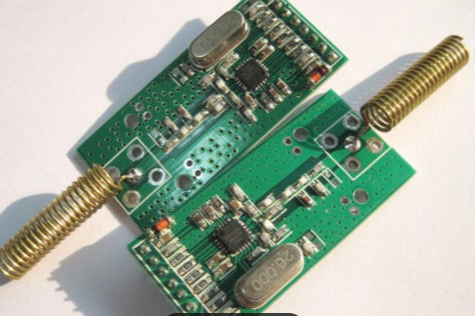
\includegraphics[width=0.4\textwidth]{Chap03/Figures/Wire_antenna.PNG}
	\caption{Wire Antenna}
	\label{WIRE_ANTENNA}
\end{figure}


\subsubsection{ PCB Antenna :}Constructively this type of antenna is copper traces
that are etched on the PCB. The Traces can be Zig-Zag, straight, MIFA, Meandered type, F-type, or Zip track so on.,
the shape of the antenna is chosen based on the antenna type and the space constraints on the PCB. PCB Antennas have only two-dimensional freedom, therefore certain guidelines are needed for the PCB antenna design due to the space constraints and poor quality of PCB stack-up.
The space constraints of the PCB antennas lead to less efficiency compared with wire antennas nonetheless PCB antennas are cost-effective.
In short manufacturing comfortability and its wireless range is ravishing for Bluetooth applications.

\begin{figure}[h]
	\centering
	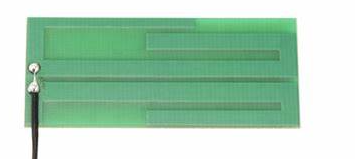
\includegraphics[width=0.4\textwidth]{Chap03/Figures/PCB_Antenna.PNG}
	\caption{PCB Antenna}
	\label{PCB_ANTENNA}
\end{figure}


\subsubsection{ Chip Antenna :} This is a Small form factor IC that is in-house with a ceramic package or some metal case.
These antennas are handier in terms of space management on the board and internally their impendence is very well managed.
A chip antenna can also take an advantage of three-dimensional freedom for radiation similar to wire antennas.
Refer to figure 10 for the Nordic Bluetooth module having a chip antenna.
Chip antennas can indeed gain upper hand in size and radion pattern on the contrary power handling capacity of the chip antenna is very minimal.
\begin{figure}[h]
	\centering
	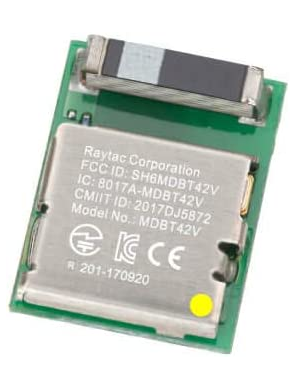
\includegraphics[width=0.4\textwidth]{Chap03/Figures/Chip_Antenna.PNG}
	\caption{Chip Antenna}
	\label{CHIP_ANTENNA}
\end{figure}



\subsection{Antenna Parameters}

The following section gives some key antenna performance parameters.

\subsubsection{Return loss :}

The return loss of an antenna signifies how well the antenna is matched to the 50-Ω transmission line (TL), shown as a signal feed in Figure \ref{fig: ANTENNA_RETUNRNLOSS}. The TL characteristic impedance is typically 50 Ω, although it could be a different value. The industry standard for commercial antennas and testing equipment is 50-Ω impedance, so it is most convenient to use this value \cite{AN91445}. \\
	
\indent  Return loss indicates how much of the incident power is reflected by the antenna due to mismatch (Equation \ref{eq:Antenna_Returnloss}).
An ideal antenna when perfectly matched will radiate the entire energy without any reflection. If the return loss is infinite, the antenna is said to be perfectly matched to the TL, as shown in Figure \ref{fig:ANTENNA_RETUNRNLOSS}. S11 is the negative return loss expressed in decibels. In most cases, a return loss ≥ 10 dB (equivalently, S11 ≤ –10 dB) is considered sufficient. Table \ref{tb:ANTENNA_RETURNlOSS_TABLE} relates the return loss (dB) to the power reflected from the antenna (percent). 
A return loss of 10 dB signifies that $90\%$ of the incident power goes into the antenna for radiation \cite{AN91445}.

\begin{equation}\label{eq:Antenna_Returnloss}
    \begin{split}
        Returnloss(db) = 10 \times \log( \frac{Pincident}{Preflected})
    \end{split}
\end{equation}

\begin{figure}[h]
	\centering
	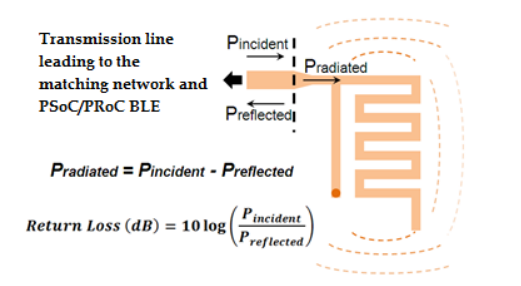
\includegraphics[width=0.65\textwidth]{Chap03/Figures/Antenna_ReturnLoss.PNG}
	\caption{Antenna Return loss}
	\label{fig:ANTENNA_RETUNRNLOSS}
\end{figure}

\begin{table}[h]
	\begin{tabular}{|c|c|c|c| }
		\hline 
		S11 (dB) & Return Loss (dB) & $\varGamma_{ref}$/$\varGamma_{inc}$t $(\%)$ & $\varGamma_{rad}$/$\varGamma_{inc}$ (\%) \\ 
		\hline
		–20 &20 &1 &99\\
		\hline
		–3 &3 &50 &50\\
		\hline
		–10 &10 &10& 90\\
		\hline
		–1 &1 &79 &21\\
		\hline
	\end{tabular}
	\caption{Return Loss and Power reflected from antenna}
	\label{tb:ANTENNA_RETURNlOSS_TABLE}
\end{table}



\subsubsection{Bandwidth :}

Bandwidth indicates the frequency response of an antenna. It signifies how well the antenna is matched to the 50-Ω transmission line over the entire band of interest, that is, between 2.40 GHz and 2.48 GHz for BLE applications \cite{AN91445}.\\

	\begin{figure}[h]
		\centering
		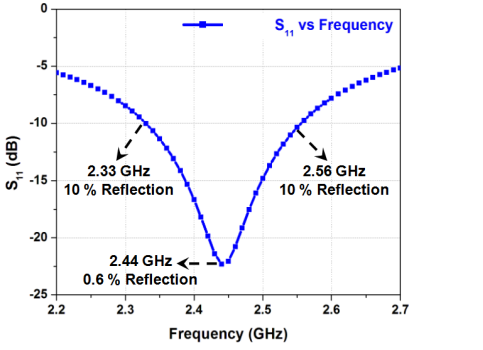
\includegraphics[width=0.65\textwidth]{Chap03/Figures/Antenna_Bandwidth.PNG}
		\caption{Antenna Bandwidth}
		\label{fig:ANTENNA_BANDWIDTH}
	\end{figure}

As Figure \ref{fig:ANTENNA_BANDWIDTH} shows, the return loss is greater than 10 dB from 2.33 GHz to 2.55 GHz. Therefore, the bandwidth of 
interest is around 200 MHz. Wider bandwidth is preferred in most cases, because it minimizes the effect of detuning 
resulting from the changes in the environments around the antenna in actual uses of the product (e.g. mouse placed 
on wood/metal/plastic table, hand kept around the mouse, etc.) \cite{AN91445}

\subsubsection{Radiation efficiency: }

A portion of the non-reflected power (see Figure \ref{eq:Antenna_Returnloss}) gets dissipated as heat or as thermal 
loss in the antenna. Thermal loss is due to the dielectric loss in the FR4 substrate and the conductor loss in the 
copper trace. This information is characterized as radiation efficiency. The radiation efficiency of 100 percent indicates 
that all non-reflected power is radiated to free space. For a small-form-factor PCB, the heat loss is minimal \cite{AN91445}.

\subsubsection{Radiation pattern:}
Radiation pattern indicates the directional property of radiation, that is, which directions have 
more radiation and which have less. This information helps to orient the antenna properly in an application \cite{AN91445}.\\


\indent An isotropic dipole antenna radiates equally in all directions in the plane perpendicular to the antenna axis. However, 
most antennas deviate from this ideal behavior. See the radiation pattern of a PCB antenna shown in Figure \ref{fig:ANTENNA_RADIATION_PATTERN} as an 
illustration. Each data point represents RF field strength, measured by the received signal strength indicator (RSSI) in 
the receiver. As expected, the contours are not exactly circular, as the antenna is not isotropic \cite{AN91445}.


\subsubsection{Gain :}
Gain indicates the radiation in the direction of interest compared to the isotropic antenna, which radiates 
uniformly in all directions. This is expressed in terms of dBi—how strong the radiation field is compared to an ideal 
isotropic antenna \cite{AN91445}.

\begin{figure}[h]
	\centering
	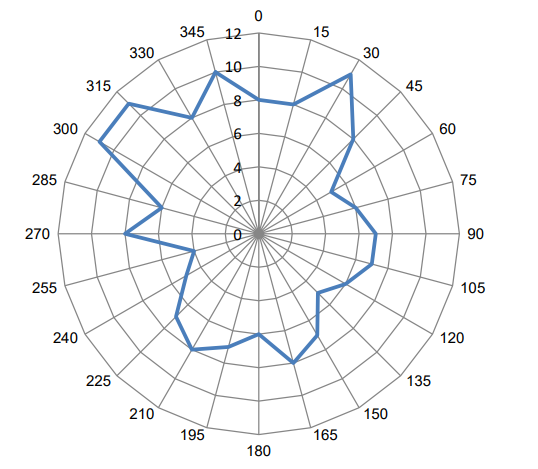
\includegraphics[width=0.65\textwidth]{Chap03/Figures/Antenna_Radiation_Pattren.PNG}
	\caption{Antenna Radiation Pattren}
	\label{fig:ANTENNA_RADIATION_PATTERN}
\end{figure}


\section{Motivation for Designing BLE Modules }
One of the core ideas of the Inventvm BMS team is to make the BMS project in a wireless communication environment, therefore the team has decided to use Bluetooth as the communication tool. Hence, finding the big sharks (Bluetooth Hardware and stack) in the Bluetooth world took quite some time, after a long investigation; we concluded to pick two important pies in the Bluetooth cake such as STM BLUeNRG-355mc \cite{BLNRG355_STEVAL_GUIDE} and Nordic nRF52840 \cite{NORDIC_nrf52840_USERGUIDE}. BlueEnergy-355mc is the jewel of our projects because it owes the advantages of very low power consumption: 3.4 mA, Receiver sensitivity, Bluetooth low energy data extensions, high data rate so on... despite having these many advantages STM does not manufacture the Bluetooth modules other than eval boards. Henceforth team has been paralyzed to outsource the required Bluetooth modules, later in the same path we found MIDARTRONICS the company that manufactures the Bluetooth modules using the STM BLUeNRGgy-355mc hardware named STORMY. Stormy is a such cutie pie, at least it helps at some extent in R \and D to prove the Wireless communication BMS architecture, but in the long run, we have experienced some the discomforts such as lack of documentation and market supply...to overcome all these issues team has decided to make inventive proprietary level Bluetooth modules fr BMS project. This gave me the perfect timing and to opportunity design RF Bluetooth modules for the project, as part of my thesis which is dedicated to wireless communication BMS.\\
\indent Nordic nRF52840\cite{NORDIC_nrf52840_USERGUIDE} is another Bluetooth hardware similar to the BlueEnergy-355Mc reason behind picking the Nordic is the open BLE stack and Robust hardware. Nordic is much more comfortable in terms of different data rates, on-chip power converters, 32-bit ARM Cortex M4F @64MHz so and forth. Nordic has also a dedicated BLE stack \cite{NORDIC_nrf52840_SOFTWARESTACK_GUIDE} that handles all power management resources on-chip, which attracts low-power automobile applications. In a much broader sense, Nordic is additional Bluetooth hardware that we can provide to the customer according to the application's need.\\
\indent Though picking the Bluetooth hardware and stack is a boiling task, choosing the antenna and RF layout also takes prime place. Though, there are plenty of antennas for the 2.4GHz band, most Bluetooth manufacturers recommend two types of PCB antennas, meanders inverted antennas (MIFA) and inverted-F antenna (IFA), which are characterized and simulated exclusively for the low-power Bluetooth applications.However, MIFA (PIFA) is peculiar for most automobile applications because of its pointed directional properties.\\
\indent, However, we can choose any type of antenna and hardware for Bluetooth, admittedly the antenna, hardware, and RF layout design described in the following modules are classified for the BMS project.\\
\indent The Low Data rate and bandwidth requirement in Bluetooth applications make IFA and MIFA the two most atractive antennas for BLE.  Manufacturing these antennas is extremely easy because they are part of the PCB design. Certainly, these antennas are inexpensive as they are part of PCB and they provide good bandwidth in ranges for BLE in terms of 150 to 250 MHZ.MIFA is most preferable for smaller form factor PCBs such as a wireless mouse, wearable watches, handy IoT devices.... etc. IFA antennas are recommended for applications such as one of the dimensions is needed to be smaller than the other for example heart rate monitor.
The following modules explain MIFA and IFA antennas construction and functionalities:

\section{PCB Meandered Inverted-F Antenna (PIFA/MIFA)}

PIFA antennas are much more popular in Bluetooth Low Energy stack because of the small size, low profile and cost-effective compared to the conventional dipole and ceramic chip antennas.
The proposed structure (PIFA/MIFA) Figure \ref{fig:MIFA_Antenna_1} of the PIFA antenna is routed to gain all these advantages.
Replacing the conventional PCB trace in PIFA with the meandering line and meandering shorting strip
improves the efficiency of the PIFA as well as the bandwidth. 
\begin{figure}[h]
	\centering
	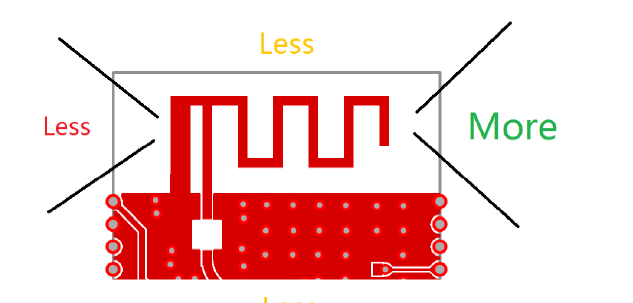
\includegraphics[width=0.4\textwidth]{Chap03/Figures/MIFA_Antenna_radiation_direction.PNG}
	\caption{MIFA/PIFA antenna radiation direction}
	\label{fig:MIFA_RADIATION_DIRECTION}
\end{figure}

Figure \ref{fig:MIFA_Antenna_1} Taking the meandered shape on one side and connecting meandered terminal to the ground makes the radiation lobe a more directional Figure\ref{fig:MIFA_RADIATION_DIRECTION} that implicates the radiation of the meandered antenna.Meandered side of the antenna radiates very less power because the Menderes terminal is connected to the ground which nullifies most of the radiation on the backward side. This kind of feature is highly needed in extremely noisy environments such as automobiles, power grid applications, data servers....etc.
As a case study, the design and measurement results of the
proposed MIFA/PIFA are presented \cite{PIFA2017Cheuk} in Figure\ref{fig:MIFA_Antenna_1}.


\begin{figure}[h]
	\centering
	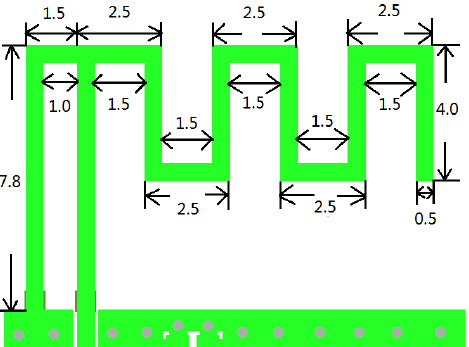
\includegraphics[width=0.65\textwidth]{Chap03/Figures/MIFA_Antenna.PNG}
	\caption{PCB Inverted Meandered F type Antenna \cite{NXP_AN11994_Antenna_Guide} }
	\label{fig:MIFA_Antenna_1}
\end{figure}

\subsection{Antenna used in Inventvm BLE modules :}
\indent I got an opportunity complete the Inventvm BLE module antenna simulation Figure\ref{fig:MIFA_Antenna_1} to depict the typical board shape and the antenna placement \cite{NXPBLE_Antenna_Guide}. The RF shield housing has been removed for testing purposes, usually, Bluetooth modules provide RF housing to protect the BLE from external interference.

\begin{figure}[h]
	\centering
	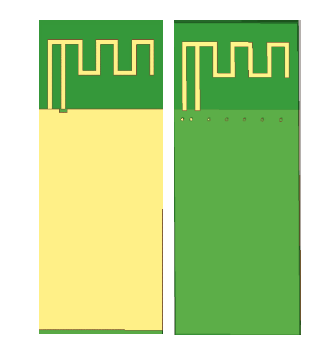
\includegraphics[width=0.4\textwidth]{Chap03/Figures/mifa_antenna_pcb_example.PNG}
	\caption{BLE module PCB with the MIFA/PIFA antenna placement}
	\label{fig:fig:PIFA_Antenna_PCB}
\end{figure}

Some MIFA/PIFA antenna and PCB parameters that are used for the simulation are shown in the table \ref{tb:MIFA_ANTENNA_SIMULATION_PARAMETERS}.

\begin{table}[h]
	\centering
	\begin{tabular}{|c|c|c| }
		\hline 
		\textbf{Antenna parameters} & \textbf{Value} & \textbf{Unit} \\ 
		\hline
		PCB substrate permittivity & 4.6 & — \\
		\hline
		PCB substrate H & 1.0 & mm \\
		\hline
		Length of PCB substrate & 35.5 &mm\\
		\hline
		Width of PCB substrate &14 &mm\\
		\hline
		Length of TOP PCB ground & 25.5& mm\\
		\hline
		Width of TOP PCB ground& 14& mm\\
		\hline
		Length of BOT PCB grounD &25.5 &mm\\
		\hline
		Width of BOT PCB ground &14 &mm\\
		\hline
		Width of antenna trace &0.5 &mm\\
		\hline
	\end{tabular}
	\caption{MIFA/PIFA antenna simulation parameters \cite{NXP_AN11994_Antenna_Guide}}
	\label{tb:MIFA_ANTENNA_SIMULATION_PARAMETERS}
\end{table}

\subsection{S11 of the MIFA/PIFA antenna}
Figure\ref{fig:MIFA_S11} shows the MIFA/PIFA antenna s11 parameter simulation results. The Bluetooth frequency bandwidth ranges from 2402 to 2483.5 MHz. The return loss of the antenna in the Bluetooth frequency band is less than the -10db.

\begin{figure}[h]
	\centering
	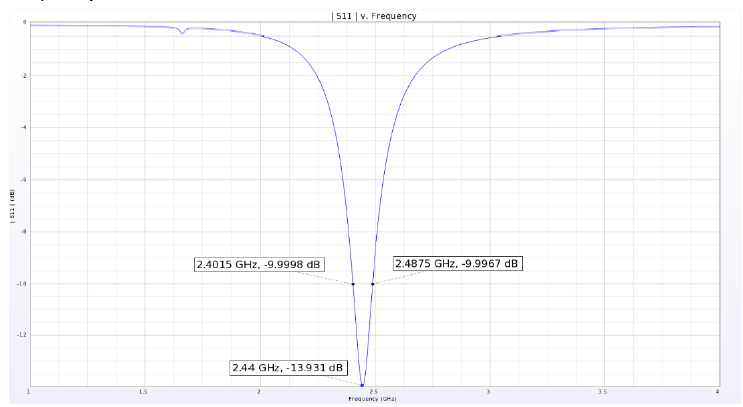
\includegraphics[width=0.7\textwidth]{Chap03/Figures/MIFA_Antenna_S11.PNG}
	\caption{MIFA/PIFA antenna S11 return loss}
	\label{fig:MIFA_S11}
\end{figure}
\begin{figure}[h]
	\centering
	\subfigure[MIFA antenna Gain Radiation pattern $@ \phi =90\deg$]{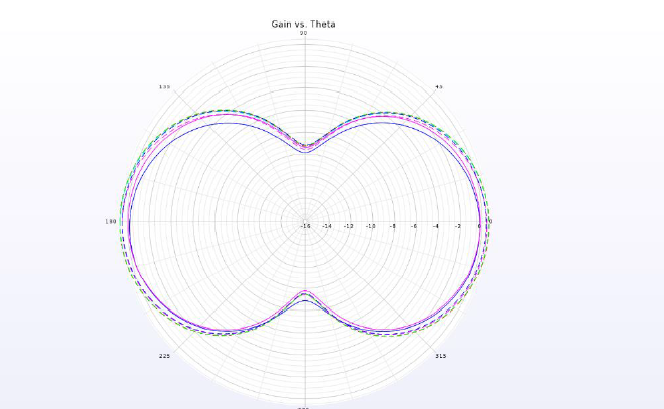
\includegraphics[scale=.5]{Chap03/Figures/mifa_Antenna_gain_pattern_phi_90.PNG}}
	\qquad
	\subfigure[MIFA antenna Gain Radiation pattern $@ \phi =0\deg$]{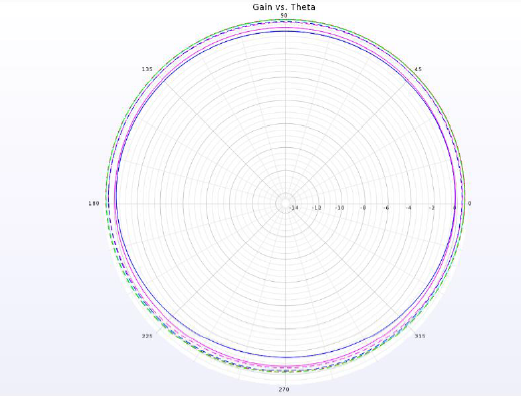
\includegraphics[scale=.5]{Chap03/Figures/mifa_Antenna_gain_pattern_phi_0.PNG}}
	\caption{MIFA Antenna Gain Radiation Pattren}
	\label{fig:MIFA_Antenna_Gain_Radiation_Pattren}
\end{figure}
\subsection{MIFA/PIFA antennas 3D pattern :}
\begin{figure}[h]
	\centering
	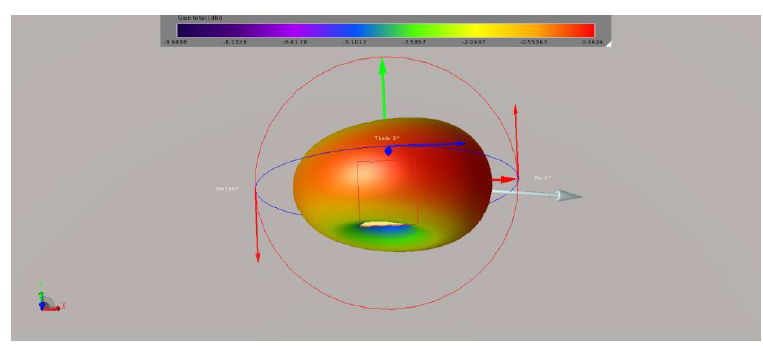
\includegraphics[width=0.7\textwidth]{Chap03/Figures/mifa_antenna_3d.PNG}
	\caption{MIFA/PIFA antenna 3D radiation Pattren}
	\label{fig:MIFA_3D}
\end{figure}

% \subsubsection{MIFA/PIFA antenna efficiency Simulation Results :}
\begin{figure}[h]
	\centering
	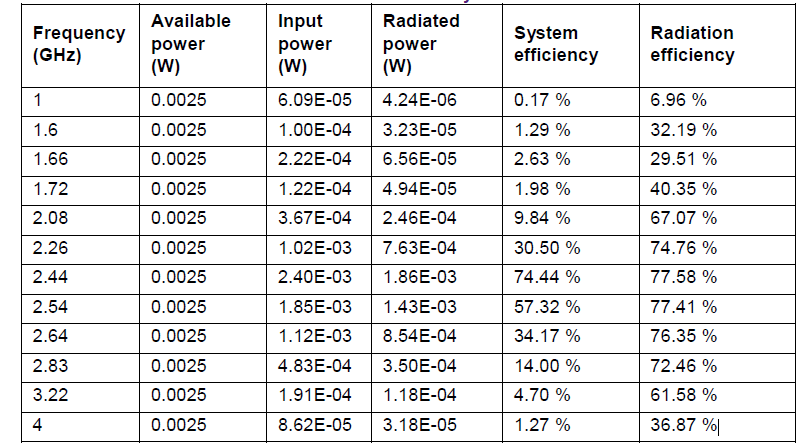
\includegraphics[width=1\textwidth]{Chap03/Figures/mifa_antenna_effieciency.PNG}
	\caption{MIFA/PIFA antenna efficiency Simulation Results}
	\label{fig:MIFA_antenna_effieciency}
\end{figure}

\section{Inverterd-F Antenna:}
The inverted F antenna is also one of the popular antennae, recommended for the Low power stack BLE applications. IFA antennas host similar features to what MIFA/PIFA antennas offer but MIFA antennas are more recommended where is a space constraint and power radiation is in one direction. IFA antennas have bidirectional power radiation rather than mono-directional. Nordic Recommends in all designs to use the IFA antennas. Figure \ref{fig:IFA_Antenna_1} educates the typical design of the IFA antenna and simulation parameters are pretty much the same as it is used for the MIFA antenna Table \ref{tb:MIFA_ANTENNA_SIMULATION_PARAMETERS}.

\begin{figure}[h]
	\centering
	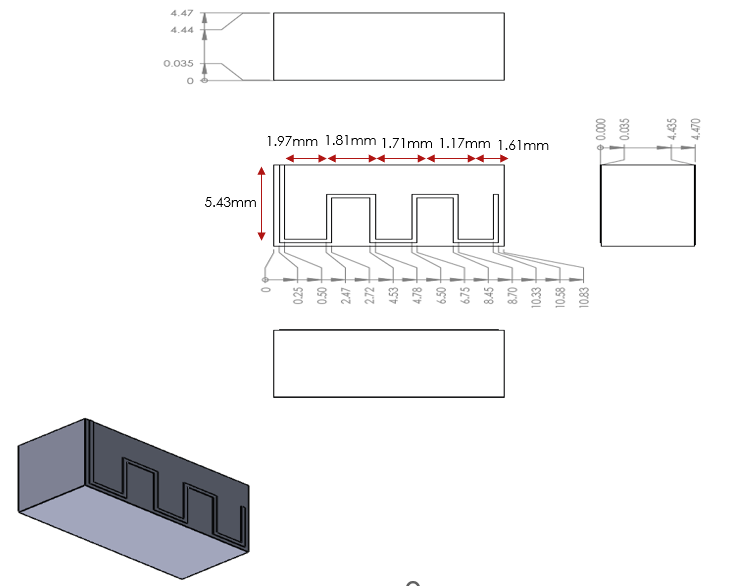
\includegraphics[width=1\textwidth]{Chap03/Figures/IFA_antenna.PNG}
	\caption{IFA antenna design and the placement}
	\label{fig:IFA_Antenna_1}
\end{figure}

By the constructional nature of the IFA antennas are easy to match we can see that in the Figure \ref{fig:IFA_Antenna_reflection} IFA antenna is very well-matched at 2.4GHz. The S11 is quite impressive because it has a reflection coefficient at 2.4GHz is -27db and bandwidth at -9db is 160MHz.
\begin{figure}[h]
	\centering
	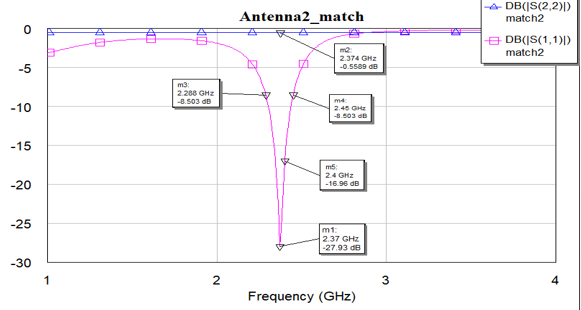
\includegraphics[width=1\textwidth]{Chap03/Figures/IFA_antenna_reflecctions.PNG}
	\caption{IFA antenna S11 and S22}
	\label{fig:IFA_Antenna_reflection}
\end{figure}
IFA antenna matching can be further tuned by varying the hinges, and length of the antennas, on contrary we need to compromise with power and resonant frequencies. Figure \ref{fig:IFA_S11_Change}shows the relative length and hinge width changes of the design Figure \ref{fig:IFA_Antenna_1} caused different frequency shfit, but they keep giving the best performance in matching.
\begin{figure}[h]
	\centering
	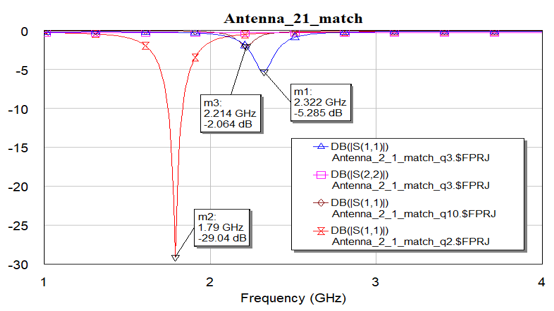
\includegraphics[width=1\textwidth]{Chap03/Figures/IFA_S11_Change.PNG}
	\caption{IFA antenna S11 Variation by changing the length and hinge width}
	\label{fig:IFA_S11_Change}
\end{figure}

% % % % % % % % % % % % % % % % % % % % % % % % % % %
% % % % % % % % % % % % % % % % % % % % % % % % % % %
\section{BLE Schematic and PCB layout}
The Schematic of the Inventvm BLE modules is inherited directly from the vendors, which are BluEnergy-355MC\cite{BLNRG355_STEVAL_GUIDE} and Nordic nRF52840\cite{NORDIC_nrf52840_USERGUIDE}. The Figure\ref{fig:Nordic_ST_modules} shows the pinout and shape of the BLE module, which is multi-purpose because of same shape and pinout from both the BluEnergy-355MC and Nordic nRF52840 modules. By having the Same pinout and shape with different Bluetooth hardware, customers can use different Bluetooth hardware stacks with the same BMS solution. This approach is nothing but the daughter and motherboard approach where the Bluetooth module becomes the daughter board and BMS MMU board and CMU boards become motherboards.

\begin{figure}[h]
	\centering
	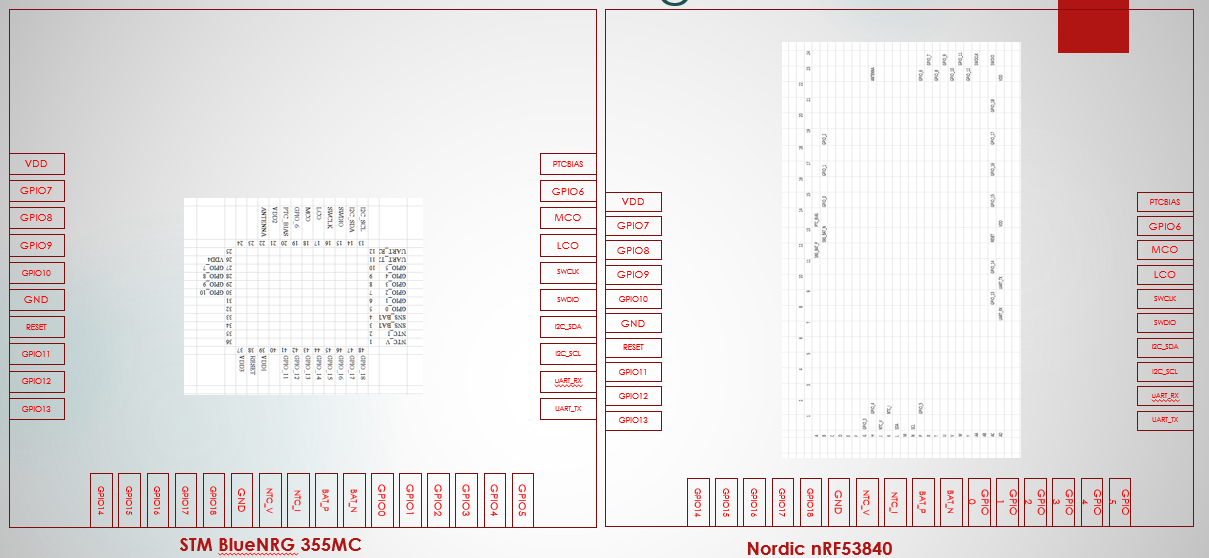
\includegraphics[width=0.7\textwidth]{Chap03/Figures/Nordic_ST_modules.PNG}
	\caption{BluEnergy-355MC(right) and Nordic Modules(left) }
	\label{fig:Nordic_ST_modules}
\end{figure}

\subsection{BluEnergy-355MC}
BLUENRG-355MC\cite{BLNRG355_STEVAL_GUIDE} BLE module includes BlueNRG-LP BLE low energy system on chip (QFN48 package), Associated with BlueNRG-LP development software stack from STM. The BlueNRG-LP features a 64 MHz, 32-bit Arm®Cortex®-M0+core, a 256 KB programmable flash memory, a 64 KB SRAM, an MPU, and an extensive peripheral set (6x PWM, 2x I²C, 2x SPI/I2S, SPI, USART, UART, PDM, and 12-bit ADC SAR)\cite{BLNRG355_STEVAL_GUIDE}. It is compliant with the Bluetooth® LE specification and supports master, slave, and simultaneous master-and-slave roles. It features data length extension, 2 Mbps, long-range, extended advertising and scanning, as well as periodic advertising, periodic advertising sync transfer, LE L2CAP connection-oriented channel, and LE power control and path loss monitoring\cite{BLNRG355_STEVAL_GUIDE}.
For more technical details refer STM BLUENRG-355MC datahseet \cite{BLNRG355_STEVAL_GUIDE}.
\subsubsection{BluEnergy-355MC RF Schematic:}
The Figure\ref{fig:STM_BLE_Schematic} refers to the core circuit of the BLUeNRG circuit for the Bluetooth, the pi network matching topology used to match the Ic and antennas, and refer \ref{fig:STM_BLE_Schematic} circuit between the RF net and the ANT net in the schematic.
All the discrete components are selected 0402 packages to make the Bluetooth module as sophisticated as possible, for more insight into the component selection for the schematic \ref{fig:STM_BLE_Schematic} refer to BOM\cite{BLNRG355_STEVAL_BOM}.
\begin{figure}[h]
	\centering
	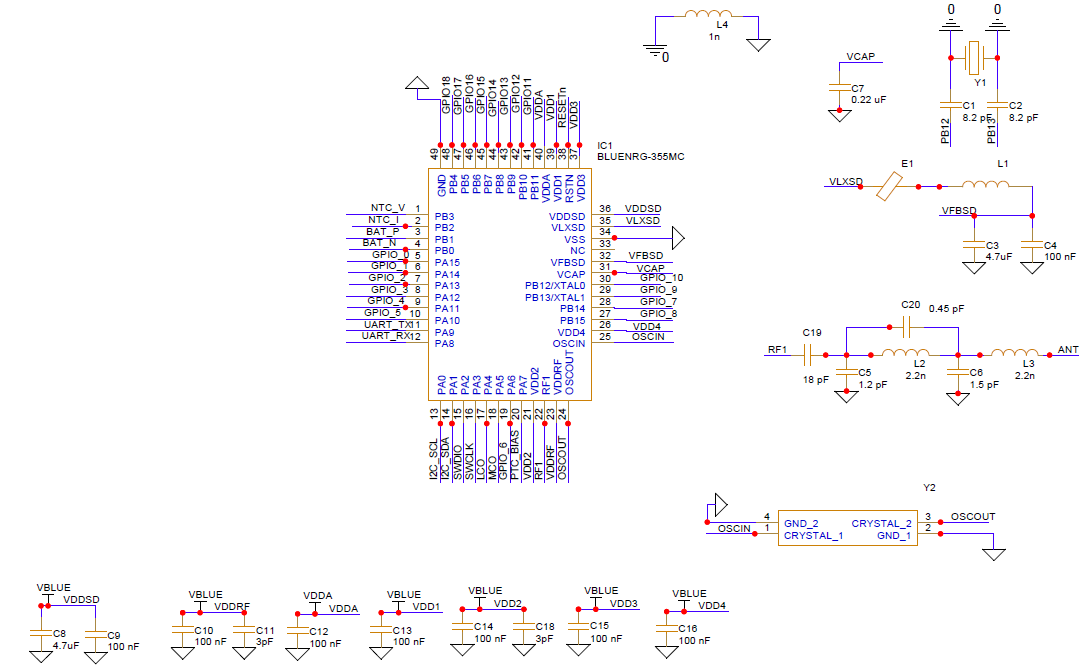
\includegraphics[width=0.7\textwidth]{Chap03/Figures/STM_BLE_Schematic.PNG}
	\caption{BluEnergy-355MC Module Core circuit }
	\label{fig:STM_BLE_Schematic}
\end{figure}

\subsubsection{BluEnergy-355MC RF Layout:}
The BLE module designed for the BMS application in Inventvm is the four-layer PCB, among four layers bottom layer is entirely dedicated to the ground. The bottom layer ground of the module is the analog ground it is differentiated from the power ground of the BMS from a small inductor to make sure the RF circuit gets less noise from the power ground. \\
\indent By referring to the layout Figure \ref{fig:BLE_PCB_ground_and_power_planes}of the RF module you can recognize that the shape of the power plane in the layer is pretty much weird, there is an RF technique behind making this kind of shape to avoid as much as the ground and power plane over a lap to decrease the capacitive parasitic effect. Parasitic components on PCB are the plague of the RF circuit, they can kill RF signal. Hence it is always a good idea to avoid power and ground planes overlap as much as possible and also make separate ground for the RF layout apart from the power ground.\\
\indent Place as many as vias possible from the top to bottom ground layer to enhance the ground layer capacity, and making sure to have equal space for antenna and RF feed line from the ground enhances the matching capability of the antenna. The following extinctions can give a detailed view of RF layout design:.

%%%%%%%%%%%%%%%%%%%%%%%%%%%%%%%%%%%%%%%%%%%%%%%%%%%%%%%%%%%%%%%%%%%%%%%%%%%%%%%%%%%%%%%%%%%%%%%%%%%%%%
%%%%% RF layout design guide lines 
%%%%%%%%%%%%%%%%%%%%%%%%%%%%%%%%%%%%%%%%%%%%%%%%%%%%%%%%%%%%%%%%%%%%%%%%%%%%%%%%%%%%%%%%%%%%%%%%%%%%%%

\begin{itemize}
	\item {\textbf{Power plane and Grounding :}}The power and Ground plane's overlap needs to be decreased as much as possible to avoid the parasitic capacitance effect. The Figure \ref{fig:BLE_PCB_ground_and_power_planes} refers to the power supply plane in the layer and the ground in the bottom layer.
		\begin{itemize}
			\noindent
			\begin{figure}[h]
				\centering
				\subfigure[Ground plane "Bottom layer"]{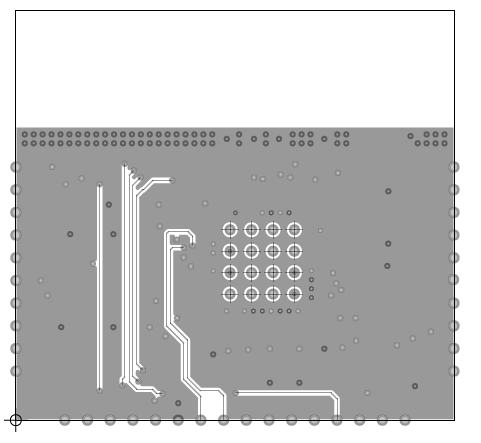
\includegraphics[scale=.6]{Chap03/Figures/nordic_module_grounding.PNG}}
				\qquad
				\subfigure[Power Plane "Layer 1"]{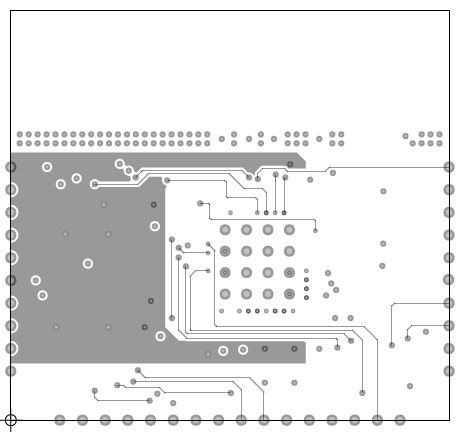
\includegraphics[scale=.6]{Chap03/Figures/Nordic_module_power_plane.PNG}}
				\caption{BLE PCB ground and power planes}
				\centering
				\label{fig:BLE_PCB_ground_and_power_planes}
			\end{figure}
		\end{itemize}
	\item \textbf{Equal Clearance to Antenna Feed :} It is essential to keep the same clearance throughout the RF feed line from the ground. This strategy helps to make equal parasitic capacitance from the ground. With an equal parasitic capacitance from the opposite side, the RF sanding wave reflections can be nullified. Figure\ref{fig:Antenna_Feed_clearence} depicts one such example of designing the RF feed line.
		\begin{itemize}
			\item \begin{figure}[h]
			    \centering
				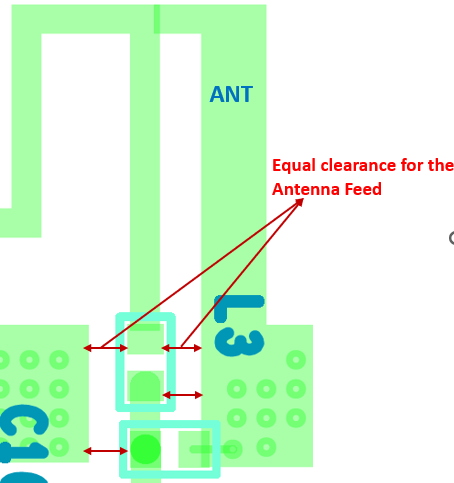
\includegraphics[width=0.4\textwidth]{Chap03/Figures/Antenna_Feed.PNG}
					\caption{Antenna Feed Line clearence}
					\label{fig:Antenna_Feed_clearence}
				\end{figure}
		\end{itemize}
	\item \textbf{ Isolate Power Ground from Analog/RF ground :}It is the most common practice while RF layout designing, The RF layout is isolated from the Power circuit. For this approach I have few intuitions behind the two-fold, those are :
		\begin{enumerate}\label{en:RFGND_isolation_benifits}
			\item RF-related noise is confined within the RF/Analog ground of the PCB.
			\item This will isolate noise from the digital circuitry with the DC power supply and High power switching circuit on the BMS board.
			\item RF circuit protected from direct current flow from DC supply if there are any power surges in supply. So on....
		\end{enumerate}
	    \begin{figure}[h]
			\centering
			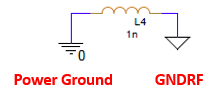
\includegraphics[width=0.4\textwidth]{Chap03/Figures/PGND_GNDRF_Isolation.PNG}
				\caption{Power Ground and RF Ground Isolated with Inductor}
				\label{fig:PGND_GNDRF_Isolation}
		\end{figure}
		\ref{en:RFGND_isolation_benifits} Such mentioned benefits can be obtained by placing an inductor between the Power Ground/RF ground. Choosing Inductor for such functionality follows that the inductor will not allow sudden current spikes $L\times \frac{d i}{d t}$ , on the benefit it can also provide a high current ratio when the current is stable,reference \ref{fig:PGND_GNDRF_Isolation}..
	\item \textbf{ RF feed line shape :}It is common practice to keep the rf feed line with the known shape. Since Bluetooth operates at 2.4GHz, even one millimeter can give a large amount of resonant frequency drift in antenna reflections. The simplest approach to mitigate such issues is to keep the RF feed and the RF IC, both on the same axis. To avoid unnecessary parasitics by an irregular shape of the antenna, make a feed trace from the ic to Antenna with the same width as the antenna feed has. Figure \ref{fig:Antenna_Feed_Shape} shows the approach that I have followed to design the Antenna feed and the RF trace, The Figure shows the nonregular shape of the antenna.
			\begin{itemize}
				\item 
				\begin{figure}[h]
					\centering
					\subfigure[Regular shape and Antenna feed]{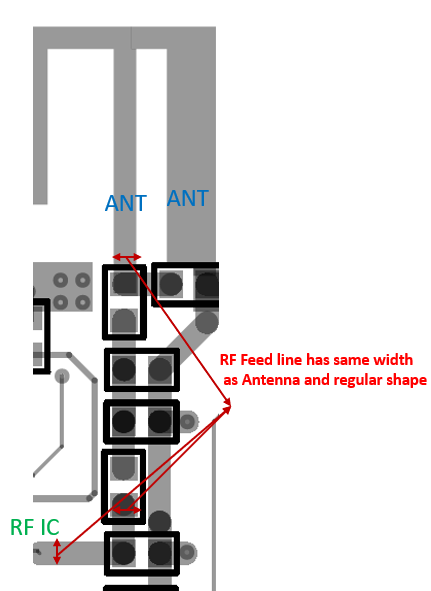
\includegraphics[scale=.6]{Chap03/Figures/Regular_Antenna_feed.PNG}}
					\qquad
					\subfigure[Irregular Antenna shape and Antenna feed]{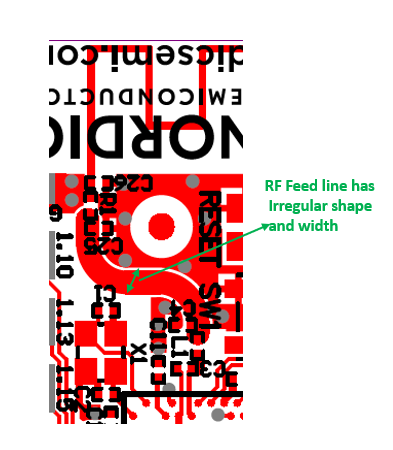
\includegraphics[scale=.6]{Chap03/Figures/Irregular_antenna_feed.PNG}}
					\caption{Antenna Feed Shape}
					\centering
					\label{fig:Antenna_Feed_Shape}
				\end{figure}
			\end{itemize}
	\item \textbf{Grounding Via's :} Keep always clean ground and this can be achieved by placing as many vias from the top layer to the dedicated RF/Analog ground in the bottom layer. It is recommended in the PCB design to place the Vias with equal distance, Figure \ref{fig:Antenna_Feed_Shape} refers to Vias placement from the top layer to the bottom layer with equal distance. There should not be any ground under the RF antenna, because the ground under the RF antenna again makes, Antenna just an RF trace instead of allowing open radiation.
	\begin{itemize}
		\item 
		\begin{figure}[h]
			\centering
			\subfigure[Top Layer Vias]{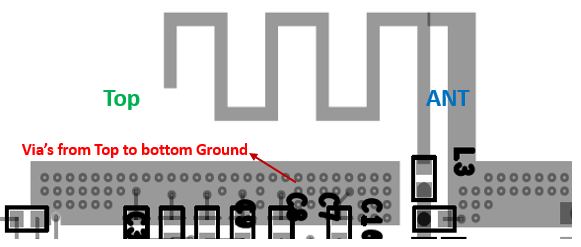
\includegraphics[scale=.5]{Chap03/Figures/Top_vias.PNG}}
			\qquad
			\subfigure[Bottom Layer Vias]{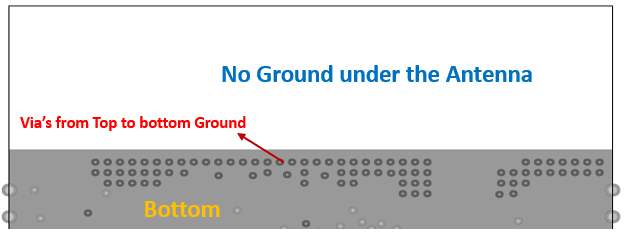
\includegraphics[scale=.5]{Chap03/Figures/Bottom_vias.PNG}}
			\caption{Vias placement on BLE board}
			\centering
			\label{fig:BLE_Module_Vias_Placement}
		\end{figure}
	\end{itemize} 
	\item \textbf{Antenna placement :} Do not place any component in the Antenna Keep out area, make the strict keep-out area for the antenna to prevent any external components' noise interference. It is always good placement to avoid any of the plastic components around the antenna because the plastic can behave like a dielectric and this will change the antenna characteristics. Antenna placement on they should end of the PCB where the PCB notch is pointed out. See Figure\ref{fig:BLE_PCB_ground_and_power_planes} the antenna has been placed on the edge of the PCB and there are no plastic or high-frequency switching circuits around it.
\end{itemize}

\subsubsection{Power Supply Decoupling Layout Considerations\cite{AN91445}}
Note the following best practices when laying out the power supply traces:
\begin{itemize}
	\item Place the components as close to the supply pin as possible \cite{AN91445}.
	\item Place the smallest-value capacitor closest to the power supply pin \cite{AN91445}.
	\item Place the decoupling capacitor on the same layer as the IC. If it is not possible to place all the capacitors on the same layer, give priority to smaller values \cite{AN91445}.
	\item The power supply should flow through the decoupling capacitors to the power supply pin of the IC. Avoid using
	\item supply vias between the component and the pin \cite{AN91445}.
	\item Use separate vias to ground for each decoupling capacitor. Do not share vias\cite{AN91445}.
	\item For four-layer boards with a separate power plane, use separate vias for each power supply pin to the power plane \cite{AN91445}.
	\item It is recommended not to share the vias \cite{AN91445}.
	\item Some of the commonly made layout issues related to power supply decoupling are shown in \cite{AN91445} Figure \ref{fig:Power_Supply_Decoupling}.
\end{itemize}
\begin{figure}[h]
	\centering
	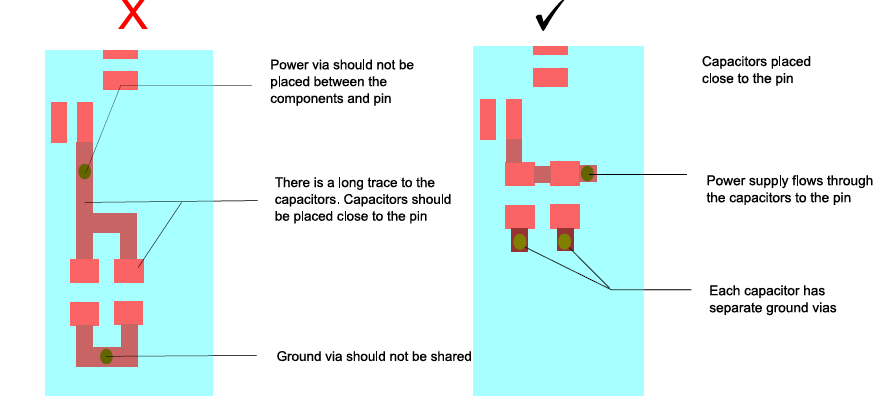
\includegraphics[width=0.7\textwidth]{Chap03/Figures/power_supply_coupling.PNG}
		\caption{Power Supply Decoupling}
		\label{fig:Power_Supply_Decoupling}
\end{figure}

%%%%%%%%%%%%%%%%%%%%%%%%%%%%%%%%%%%%%%%%%%%%%%%%%%%%%%%%%%%%%%%%%%%%%%%%%%%%%%%%%%%%%%%%%%%%%%%%%%%%%%

\subsubsection{BluEnergy-355MC RF Matching Circuit Layout:}
It is always a good approach to have the matching circuit as tight as possible you can refer to the Figure\ref{fig:Antenna_matching_network} the matching circuit is placed as close as possible, to avoid any additional track length to create some extra RF stub effects.  Don't ever run any of the signal lines across the RF feed line and always make sure to place the IC and RF in the same direction this approach will avoid any strange track shapes which can cause parasitics. It is a good way to make sure the RF feed line to the antenna through the IC has the same width across the track length this will avoid any unnecessary filtering effect. The figure refers to all of above-mentioned RF layout design hints.
Figure\ref{fig:Antenna_matching_network} shows that matching components are tightly packed, and no signals run across the RF feed.

\begin{figure}[h]
	\centering
	\subfigure[Matching Network Layout]{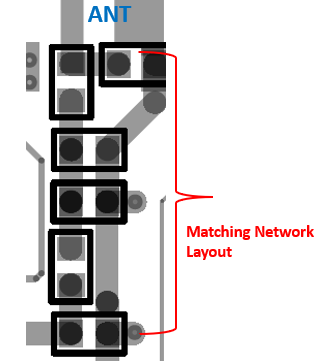
\includegraphics[scale=.8]{Chap03/Figures/matching_network_layout.PNG}}
	\qquad
	\subfigure[Matching Network Schematic]{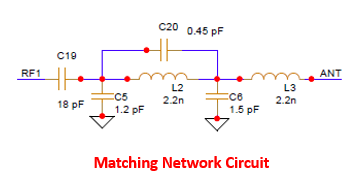
\includegraphics[scale=.8]{Chap03/Figures/matching_network_circuit.PNG}}
	\caption{BLE Antenna Matching Network}
	\centering
	\label{fig:Antenna_matching_network}
\end{figure}
We can place the components even overruling the component outline. Until we do not make the pads overlap, to achieve this we might have to bypass some PCB DRCs.

\subsection{Summary of the RF layout Design guidelines :}
\begin{enumerate}
	\item Keep Ground clearance as much as possible around the antenna.
	\item Make equi clearance on both sides of the antenna and RF feed line.
	\item Do not make a strange shape of the antenna feed line.
	\item Do not run any of the signal lines under the antenna or RF feed line.
	\item Make more vias from the top layer to the bottom layer for pure ground.
	\item Keep capacitive filters as near as possible to the power supply pins.
	\item Pack antenna matching network as close to antenna and IC RF feed.
	\item Place antennae in less clumsy are from other circuitry on the PCB.
	\item Make less overlap of the ground plane and power plane.
	\item Avoid high-frequency circuits around the RF feed.
	\item Always places the antenna at the edge of the PCB.
	\item Always chooses a standard pattern for the ground around the antenna.
	\item Never places any components, screws, mounting holes, or planes in the keep-out area of the antenna.
	\item The antenna must house with a Metalic shield to avoid external interference.
	\item There should not be direct ground under the antenna.
	\item The Orientation of the antenna should be inlined with the final PCB.
	\item When using the passive matching circuit try to have multiple components matching this can help at the debugging stage to tune the matching circuit.
\end{enumerate}



\section{Conclusion of the Chapter \ref{chap:BLE}}
The simulation and design of both the MIFA and IFA antennas are successful the results have been presented in Chapter\ref{chap:BLE}.  
Both the MIFa and IFa antennas are well performed in the sense of the results and design, because of the industry standards and Bluetooth stack recommendations, from vendors I have opted MIFA for Inventvm Bluetooth modules. 
The Layout is also quite impressive considering all norms of RF PCB layout guidelines, which are mentioned in the chapter\ref{chap:BLE}.
In the chapter\ref{chap:BLE} I have not stressed the theoretical calculation for the MIFA/IFA antenna because the calculations are pretty much the same as the standard MIFA and IFA antennas, 
The goal is to bring up the sophisticated RF BLE layout according to the application with a standard approach. Yet reference papers [\cite{MIFA_Design_Losito},\cite{MIFA_IFA_difference_Kanan}] give more insight into the theocratical design of the MIFA / IFA antenna and 
I have taken fewer opportunities to explain the nordic architecture, because of the RF layout out-wise and in the antenna sense, I have followed the same guidelines as I did for the BLUeNRG-355mc.
The Complete layout of the BLUeNRG and Nordic is attached in the chapter\ref{chap:miselleneous} , Figures (\ref{fig:BLUeNRG-355mc_BLE_Layout},\ref{fig:Nordic_nrf52840_BLE_Layout}).
\thispagestyle{empty}
\cleardoublepage
% % % % % % % % % % % % % % % % % % % % % % % % % % %
% % % % % % % % % % % % % % % % % % % % % % % % % % %
% % % % % % % % % % % % % % % % % % % % % % % % % % %
% % % % % % % % % % % % % % % % % % % % % % % % % % %
\chapter{Architecture of Active Balancing Wireless Communication BMS}\label{ch:Architecture_Active_Balancing_BMS}
\section{Introduction}
\section{Active Balancing Methods}
\section{Overview of Active balancing BMS Architecture}
\section{Hardware Implementation}
\subsubsection{Multiphase Bidirectional DC/DC Current Controller LM5170-Q1}
\indent The LM5170-q1 controller is a high precision dual channel bidirectional converter applicated in automotive 48 Volts and 12Volts dual battery systems. Depending on the Direction Signal DC/DC converter regulates the average current. The Regulated current through the DC/DC converter can be programmed by analog or Digital PWM inputs.

The LM5170-q1 has a dedicated dual channel differential current sense amplifier to monitor the current flowing through the Dc/Dc converter, which can achieve $1\%$ current sense accuracy. It has a Robust Gate driver to drive half the bridge. The Internal gate driver of the LM5170 has the capability of driving parallel MOSFET switches with a capacity of 500Watts. The synchronous diode emulation mode prevents the dc to dc converter from the negative currents and also enables the discontinuous mode of operation. This property enhances the DC/DC converter efficiency tremendously. The Controller can offer benefits of cycle-by-cycle current limitation, overVoltage protection at both low side and high side ports, Temperature protection and Mosfet failure so on...
x
% \subsubsection{Matrix Switch Gate Driver :}
Modern BMS application is suffocated by the hot swapping of the Batteries for balancing. When the battery node is switched in the battery pack to balance the battery node matrix(switching circuit) the MMU will see an immense current that is flowing from the battery \cite{LTC4231_User_Datasheet}. when the switch matrix is switched to a particular node of the battery pack. The battery Node will be directly connected to the output node of the DC/DC converter (The low side of the DC/DC Converter refers to the circuit \ref{fig:Typical Bidirectional circuit of the LM5170} @low side), which will be having reservoir capacitor that will sink an immense amount of the current from the battery in very short time this will cause switching FET to burn, so it essential to switch FET very carefully. such technique is called "Hot Swap". "Hot Swap" is FET switching technique Figure\ref{fig:Mosfet_Switch_Matrix}, more often used in live power switch applications. The technique allows the gate driver circuit to monitor the current flowing through the switch circuit by the input sense resistance. By any chance Hot swap circuit doesn't allow the rapid surge of the load current in the switch circuit \cite{LTC4231_User_Datasheet}.
\paragraph{LTC4231 :}
LTC4231 is an Analog Device Inc Micro power hot-swap controller that is employed to face circuit board insertion and abrupt live power supply. An internal high-side switch driver controls the gate of an external N-channel MOSFET. Back-to-back MOSFETs can be used for reverse supply protection down to –40V \cite{LTC4231_User_Datasheet}.

The LTC4231 provides a debounce delay and allows the GATE to be ramped up at an adjustable rate. After startup, the LTC4231's quiescent current drops to 4µA during normal operation with output active. UVL, UVH, OV, and GNDSW monitor overvoltage and Undervoltage periodically, keeping total quiescent current low. Pulling SHDN low shuts down the LTC4231 and the quiescent current drops to 0.3µA.

During an overcurrent fault, the LTC4231 actively limits current while running an adjustable timer \cite{LTC4231_User_Datasheet}. The LTC4231-1 remains off after a current fault while the LTC4231-2 automatically reapplies power after a cool-down period\cite{LTC4231_User_Datasheet}.

A typical circuit diagram and the operational waveforms of the LTC4231 are described in the Figure\ref{fig: LTC4231 Application circuit and the Operational waveform}. 
For more technical details refer to the ADI LTC4231 datasheet\cite{LTC4231_User_Datasheet}.

\paragraph{Inrush Control by LTC4231 :}
In most, automotive applications keeping the inrush current low and in control is essential to avoid catastrophic damage to the switching circuits. LTC4231 takes a golden hand in controlling the inrush current by startup method (Timer Delay varying). The equations \ref{eq:LTC4321_Inrush_current} implicate the Inrush current controlled by the LTC, the Inrush current highly depends on the gate capacitance of the switch, and the output capacitance of the DC/DC capacitance (load Capacitance $C_L$). A capacitor $C_G$ of the Gate to the GND can be used to control the gate voltage slew rate for the Inrush current in the Switch.
\begin{equation}\label{eq:LTC4321_Inrush_current}
    I_{InRsush} = \frac{C_{L}}{C_{G}} \times 10\mu A
\end{equation}
\begin{figure}[h]
	\centering
	\makebox[\textwidth]{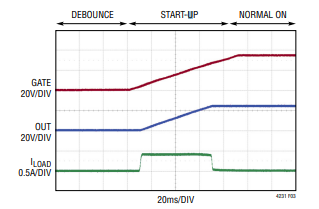
\includegraphics[width=0.9\paperwidth]{Chap04/Figures/Inrsuh_current_of_LTC4321.PNG}}
    \caption{Inrush Control by Limiting $V_{GATE}$ Slew}
    \label{fig: LTC4231 Inrush Control by Limiting VGATE Slew }
\end{figure}
The $V_{GATE}$ of the switch raise with the slope of $10\mu A/C_G$ Figure\ref{fig: LTC4231 Inrush Control by Limiting VGATE Slew}.
Once $V_{GATE}$ crosses the Vth, status goes high impedance. see the figure\cite{fig: LTC4231 Inrush Control by Limiting VGATE Slew} which explains the Inrush current protection when the $\Delta V_{Th(GATE)}$ crosses the gate voltage threshold.

The Design Example in the Chapter\ref{chap:miselleneous} explains, how to pick the design parameters to design the inrush current limit and gate driver, please follow. LTC4231 holds a wide range of advantages compared to the gate driver that is available in the market such Wide Operating Voltage Range: 2.7V to 36V, Reverse Supply Protection to –40V n Adjustable Analog Current Limit with Circuit Breaker n Automatic Retry or Latchoff on Current Fault n Overvoltage and Undervoltage Monitoring n Controls Single or Back-to-Back N-Channel MOSFETs \cite{LTC4231_User_Datasheet}. By considering all the facts we have picked the LTC4321 as the gate driver for the switch matrix.
\thispagestyle{empty}
\cleardoublepage
% % % % % % % % % % % % % % % % % % % % % % % % % % %
% % % % % % % % % % % % % % % % % % % % % % % % % % %
% % % % % % % % % % % % % % % % % % % % % % % % % % %
% % % % % % % % % % % % % % % % % % % % % % % % % % %
\chapter{Battery Emulator Setup}
% \stepcounter{chapter}\addcontentsline{toc}{chapter}{Simulink Modeling and Verification}

\section{Introduction}
The block specifications obtained from the Simulink model is considered as a starting point for the circuit level design in the Cadence. The core part of the architecture of the Extended-Range ADC to be implemented, as shown in Fig. \ref{fig:prop_eradc_circ}, consists of two integrators, 3-bit quantizer, 3-bit DAC and Inter-Stage Gain block. While the supporting-blocks required for the complete implementation are the biasing for the op-amps in the two integrators and the ISG, timing block to generate clock phases and some control signals, the Dynamic Element Matching (DEM) block for the suppression of the harmonics due to DAC unit element mismatch and the Wallace tree encoder to convert the thermometer code to binary code which is read outside for the post-processing.

%
\begin{table}[h]
\centering
\begin{tabular}{c|c|c|c}
\Xhline{4\arrayrulewidth}
\textbf{Sr. No.} & \textbf{Parameter} & \textbf{First Op-Amp} & \textbf{Second Op-Amp} \\ \hline
1 & Gain (dB) & 50 & 50 \\ \hline 
2 & GBW (MHz) & 190 & 160 \\ \hline
3 & Slew Rate (V/µs) & 190 & 160 \\ \hline
4 & Voltage Swing (V) & 0.3 & 1.2 \\ \Xhline{4\arrayrulewidth}
\end{tabular}
\caption{Op-Amp specification requirements}
\label{tab:opamp_specs}
\end{table}
%
It can be observed from Fig. \ref{SNR_G1} and Fig. \ref{SNR_G2}, though the low frequency gain requirement for the case $N_{SD}=3$ and $N_{RS}=5$ to achieve maximum SNR of 86~dB is around 80~dB, there is no significant degradation in SNR, if gain drops down to 50~dB. This relaxation in the gain requirement then helps to achieve the GBW value. The Table.\ref{tab:opamp_specs} shows the first and the second op-amp requirements for given specifications for the ADC architecture.
% \begin{table}[h]
% \centering
% \begin{tabular}{c|c|c|c}
% \hline \xrowht{15pt}
% \textbf{Sr. No.} & \textbf{Parameter} & \textbf{First Op-Amp} & \textbf{Second Op-Amp} \\ \hline\xrowht{10pt}
% 1 & Gain ($dB$) & 60 & 60 \\ \xrowht{10pt}
% 2 & GBW ($MHz$) & 250 & 140 \\ \xrowht{10pt}
% 3 & Slew Rate ($V/\mu s$) & 250 & 120 \\ \xrowht{10pt}
% 4 & Voltage Swing ($V$) & 0.3 & 1.2 \\ \hline
% \end{tabular}
% \end{table}
\section{Integrators}
%
\begin{figure}[ht]
\centering
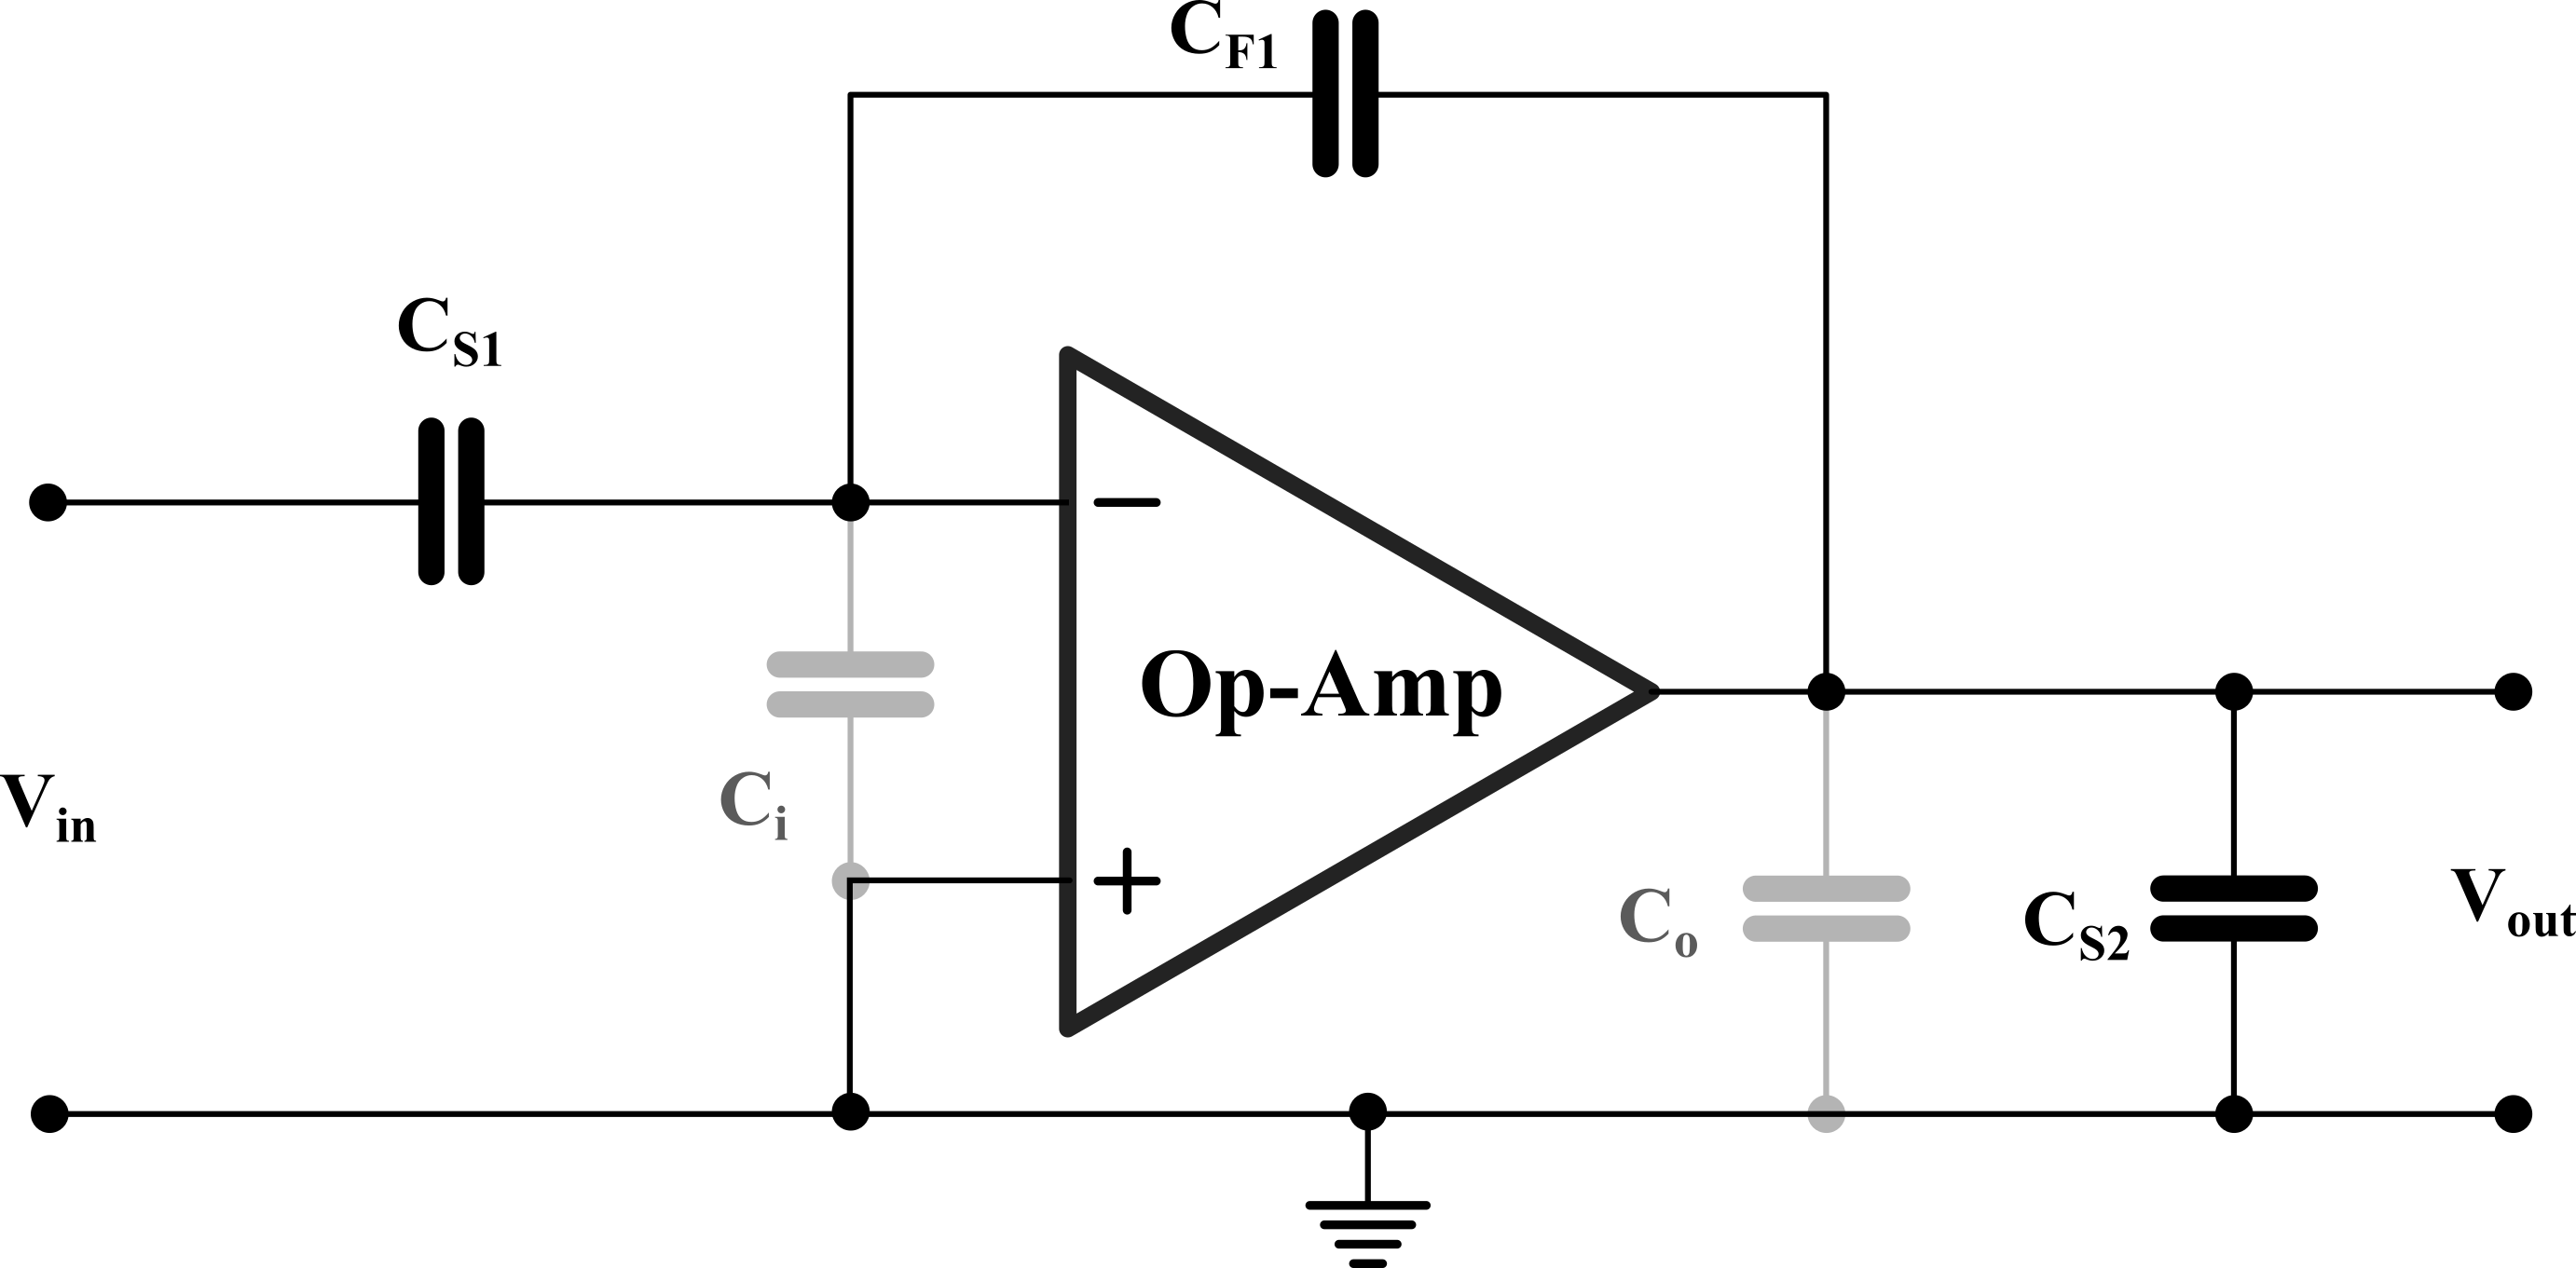
\includegraphics[width=0.6\columnwidth]{Chap05/Figures/integrator.png}
\caption{Single Ended representation of the First Integrator in the integrating phase}
\label{INT1_INTPHS}
\end{figure}
%
The choice of the architecture of the op-amps has various design constraints like power consumption, gain, GBW and slew rate, load capacitance, voltage swing etc. Two-stage op-amp is usually preferred when the gain high requirement has to be fulfilled and the power consumption is not of the concern. It also achieves high output voltage swing since at the output stage, there are just two transistors in stack. However, if along with gain the power consumption and GBW are also important, the solution could be the telescopic amplifier. Nevertheless, stack of 5 transistors between the rails in the telescopic structure limits the swing at the output. But considering the requirement, it is a good option for the op-amp in the first integrator. Swing of the signal at the output of second integrator is considerably high. Therefore, the op-amp structure or the constraints for the second integrator can be reconsidered if similar op-amp architecture has to be reused.

\subsection{Op-Amp for the First Integrator:}
In the integrating phase of the circuit of the first integrator appears like one shown in Fig. \ref{INT1_INTPHS} where $C_{S1}$ is the sampling capacitor, $C_{F1}$ is the feedback capacitor of first integrator, $C_{i}$ is the parasitic capacitor at the virtual ground node, $C_{o}$ is the parasitic capacitor at the output node of the op-amp and $C_{S2}$ is the sampling capacitor of the second integrator. The value of the sampling capacitor $C_{S1}$ is $400\ fF$, therefore the value of the feedback capacitor is also kept $400\ fF$ for the purpose to keep coefficient of the integrator to 1. 
%
\begin{figure}[h]
\centering
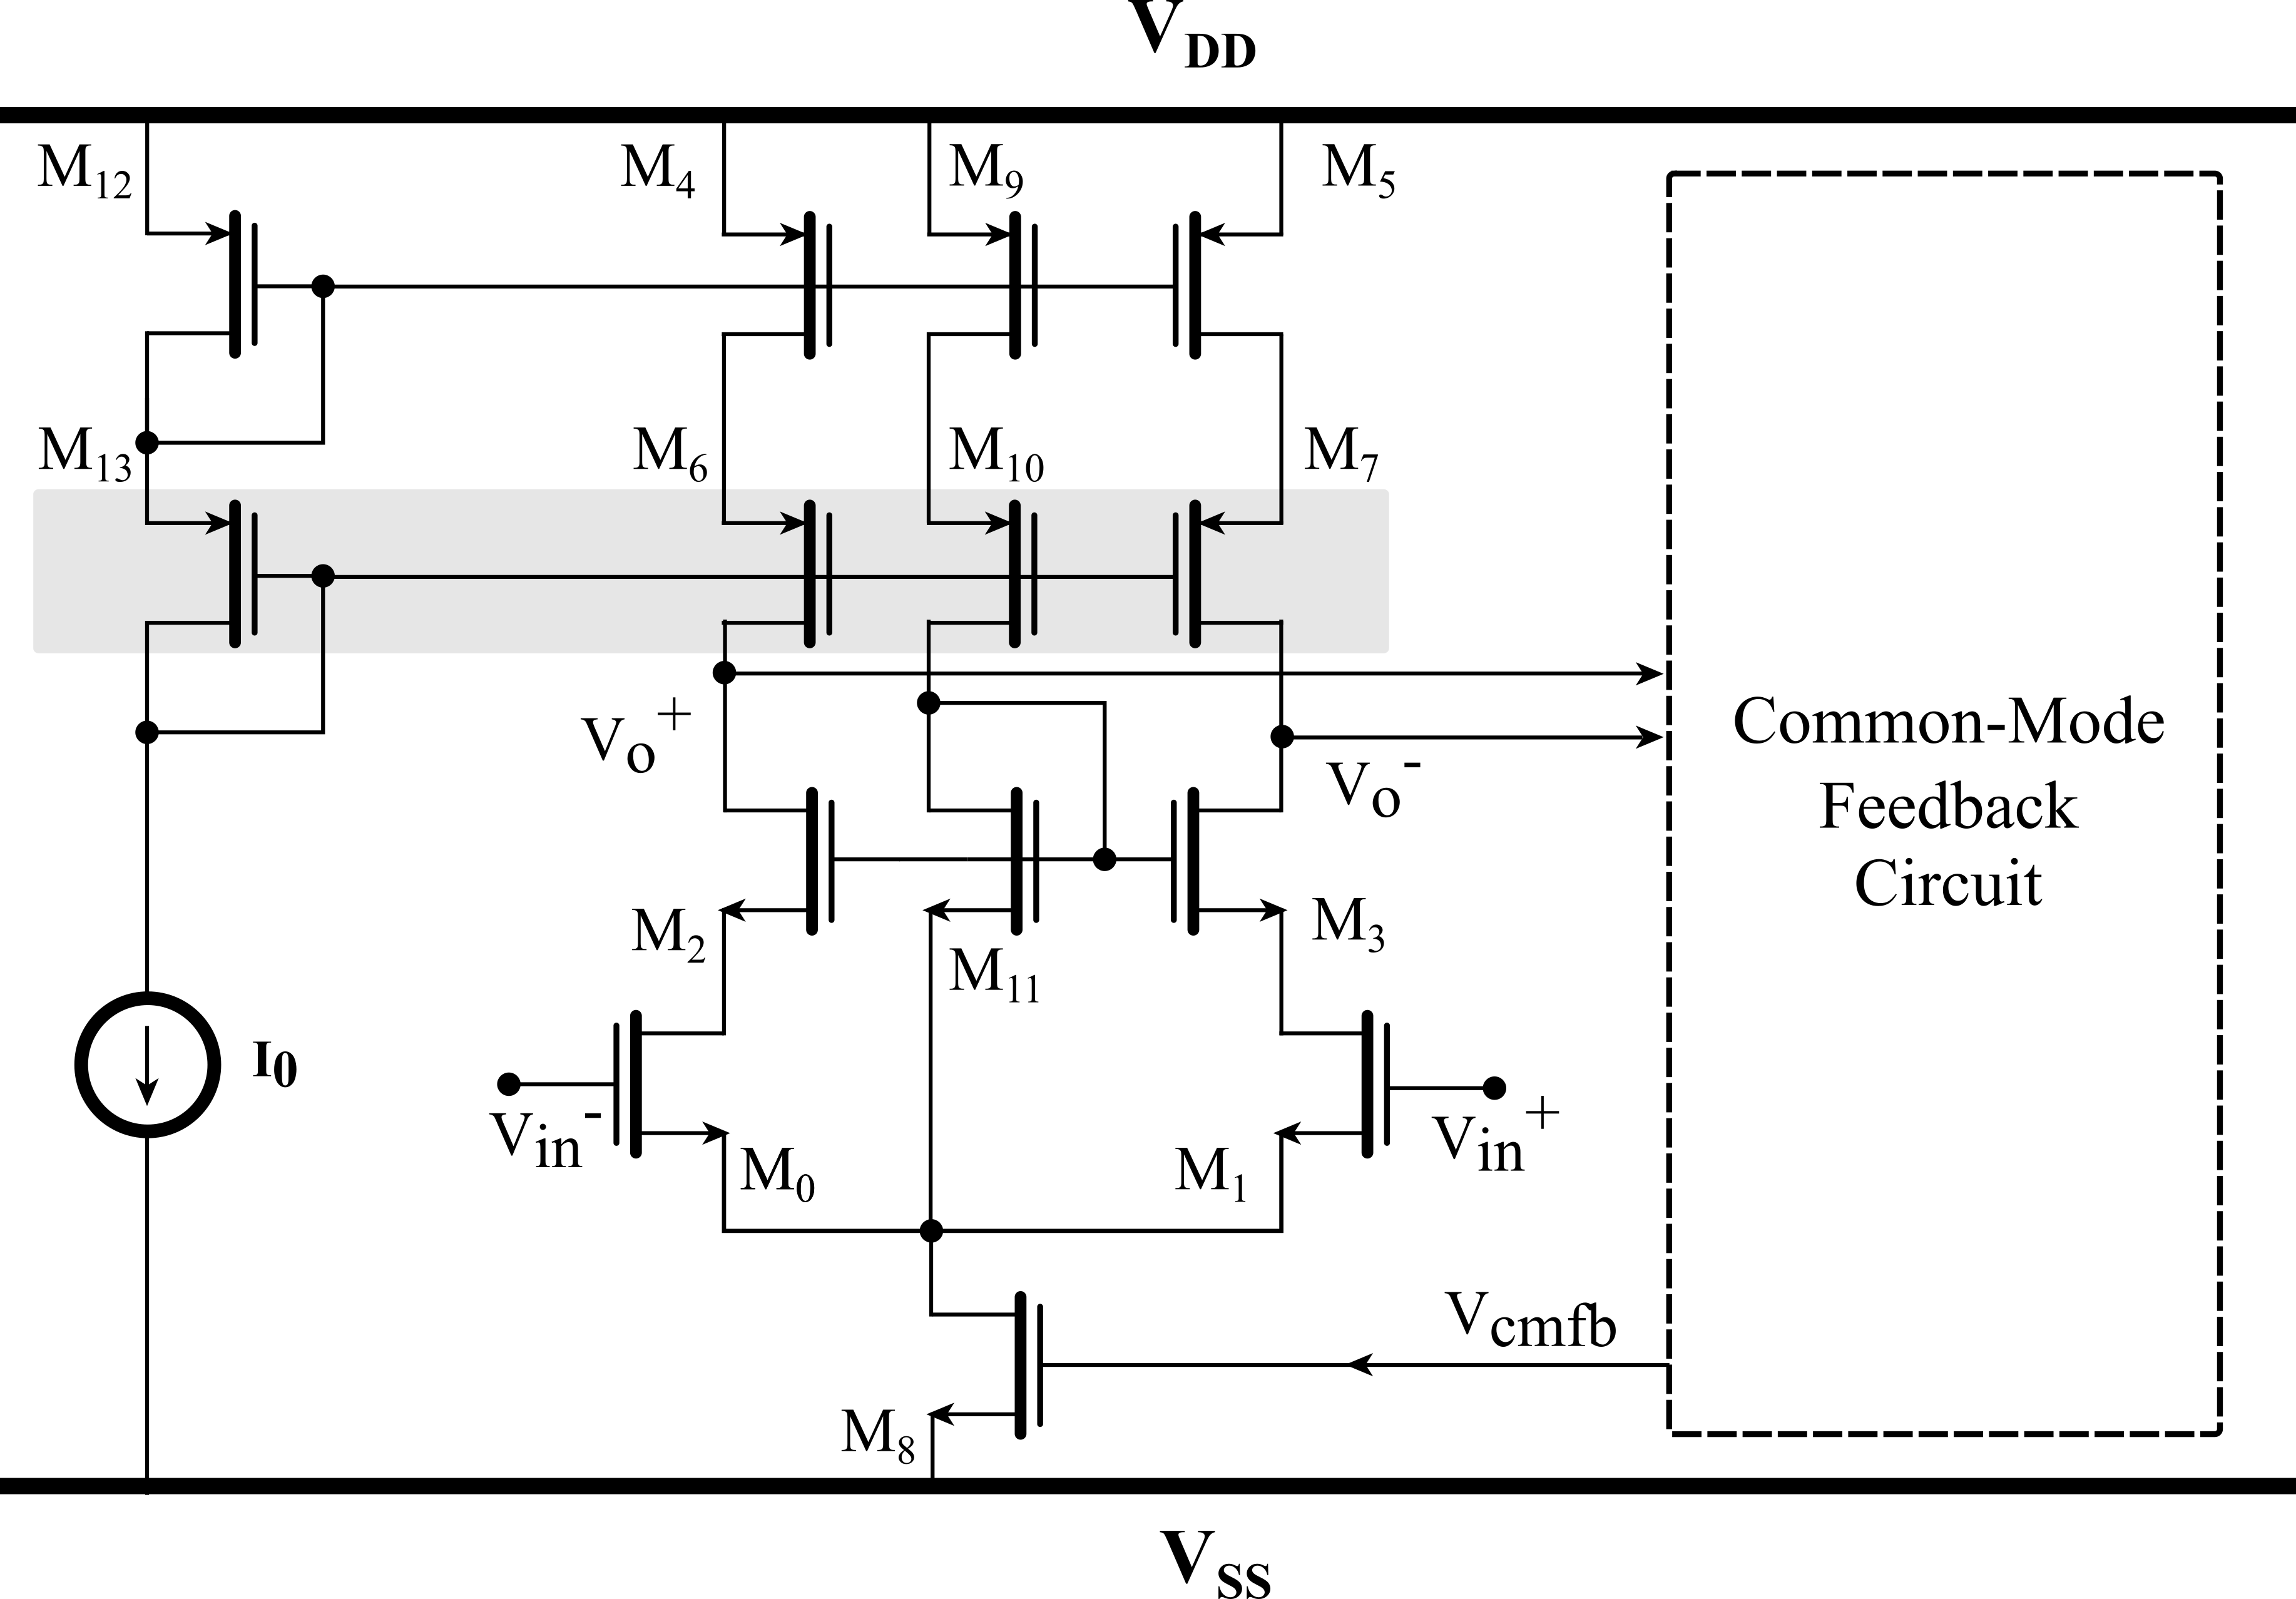
\includegraphics[width=0.85\columnwidth]{Chap05/Figures/telescopic.png}
\caption{Conventional Telescopic Amplifier Circuit Diagram}
\label{fig:TELE_AMP}
\end{figure}
%

% Similarly the value of sampling cap of the second integrator is also kept $400\ fF$, while that for $C_{i}$ and $C_{o}$ are assumed to be $100\ fF$ (assumption, prior to the design). 
From the setup in Fig. \ref{INT1_INTPHS}, the load capacitance $C_L$ and the feedback factor $\beta$, for the first integrator, can be estimated as,
\begin{equation}
    C_{L1}=\frac{C_{F1}\left(C_{S1}+C_{i}\right)}{C_{F1}+C_{S1}+C_{i}}+C_{o}+C_{S2}
    \label{CL1}
\end{equation}
\begin{equation}
    \beta_{1}=\frac{C_{F1}}{C_{F1}+C_{S1}+C_{i}}
    \label{BETA1}
\end{equation}

Making the use of the equations above, the load capacitance and the feedback factor turns out to be around $725\ fF$ and 0.44 respectively. Consequently, the design of the first op-amp has to be done to ensure the loop gain of $60\ dB$, loop GBW of $190\ MHz$, SR of $190\ V/\mu s$ and voltage swing of $300\ mV$ for the load of $725\ fF$ and $\beta$ of 0.44. 
%
\begin{equation}
    Loop\ GBW = \beta_1 \ GBW_{OL} = \beta_1 \frac{g_m}{2\pi C_{L1}}
\end{equation}
%
%
\begin{equation}
    Loop\ Gain = \beta_1\ A_{OL}
\end{equation}
%
%
\begin{figure}[h]
\centering
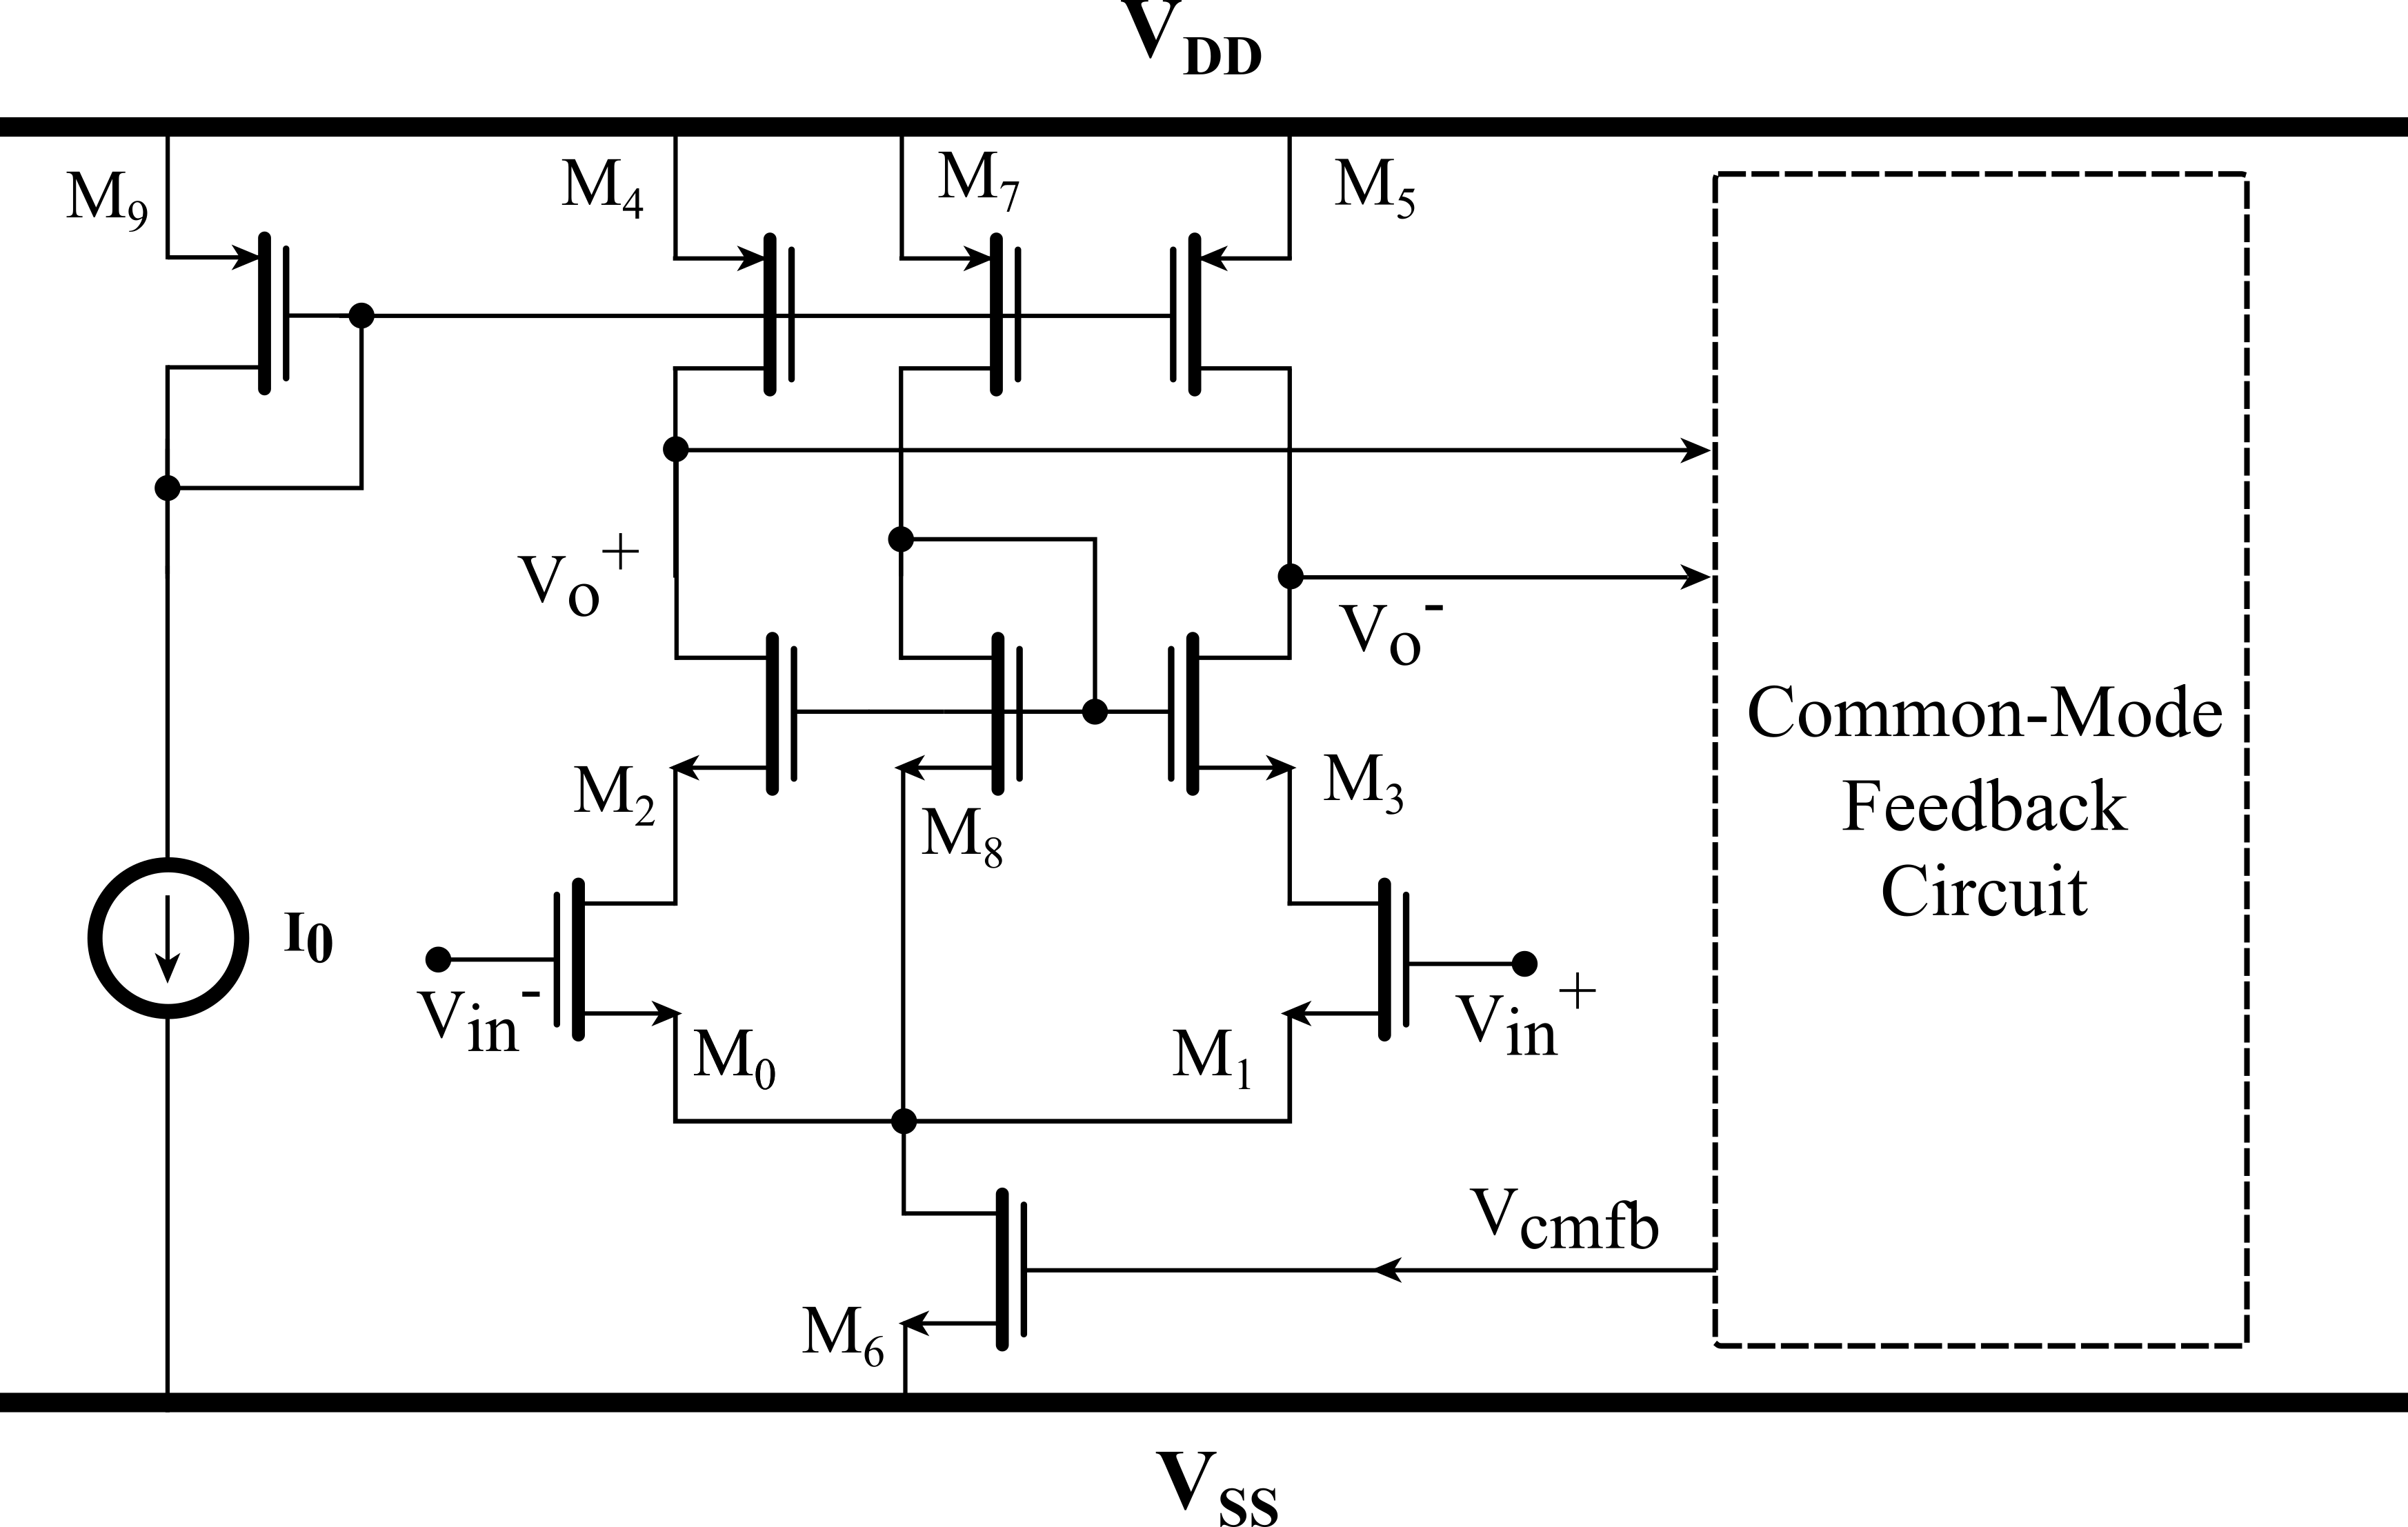
\includegraphics[width=0.9\columnwidth]{Chap05/Figures/telescopic_m.png}
\caption{Modified Telescopic Amplifier for improved output swing}
\label{TELE_AMP1}
\end{figure}
%
Two stage op-amps usually consumes more power compared to single stage op-amps, therefore the choice of single stage op-amp is made. But reduction in power comes with a drawback of reduced low frequency gain. Telescopic amplifier is the suitable alternative with the objective to overcome this drawback. In case of Telescopic amplifier, total five transistors are in stack from rail to rail (two transistors more compared to simple differential amplifier) which limits the output swing by two overdrives w.r.t. single stage differential amplifier as shown in Fig. \ref{fig:TELE_AMP}. The approach to improve the output swing can be to eliminate the one transistor from the stack highlighted in conventional structure and cause to raise it by one overdrive (Fig. \ref{TELE_AMP1}). However, the elimination of the transistor in stack leads to the lowering the gain and thus necessitates to investigate the technique to resolve this problem.


The expression for the low-frequency gain of the telescopic amplifier shown in Fig. \ref{fig:TELE_AMP} is given as,
%
\begin{equation}
    A_0 \approx g_{m0,1}\left(g_{m2,3}r_{O2,3}r_{O0,1}||g_{m6,7}r_{O6,7}r_{O4,5}\right)
\end{equation}
%
However, the elimination of the transistor from the stack reduces the output resistance, which in turn brings the low frequency gain, down. The expression for the low frequency gain and GBW of the modified telescopic amplifier for improved swing,
%
\begin{equation}\label{eq:A_0_swing_improve}
    A_0 \approx g_{m0,1}\left(g_{m2,3}r_{O2,3}r_{O0,1}||r_{O4,5}\right)
\end{equation}
%
%
\begin{equation}
    GBW = \frac{g_{m0,1}}{2\pi C_L}
\end{equation}
%
\subsection{Gain and GBW Enhancement:}
A technique is employed where the Auxiliary op-amp is incorporated for the purpose of gain enhancement\cite{ISCAS_PEREZ} as shown in the block diagram Fig. \ref{BLK_GIN_ENH}. Auxiliary op-amp takes same inputs as the principal one and generates the signals which in turns, are used to drive the main op-amp. The power consumption of the auxiliary op-amp is significantly lower than that in the principal one.
\begin{figure}[h]
\centering
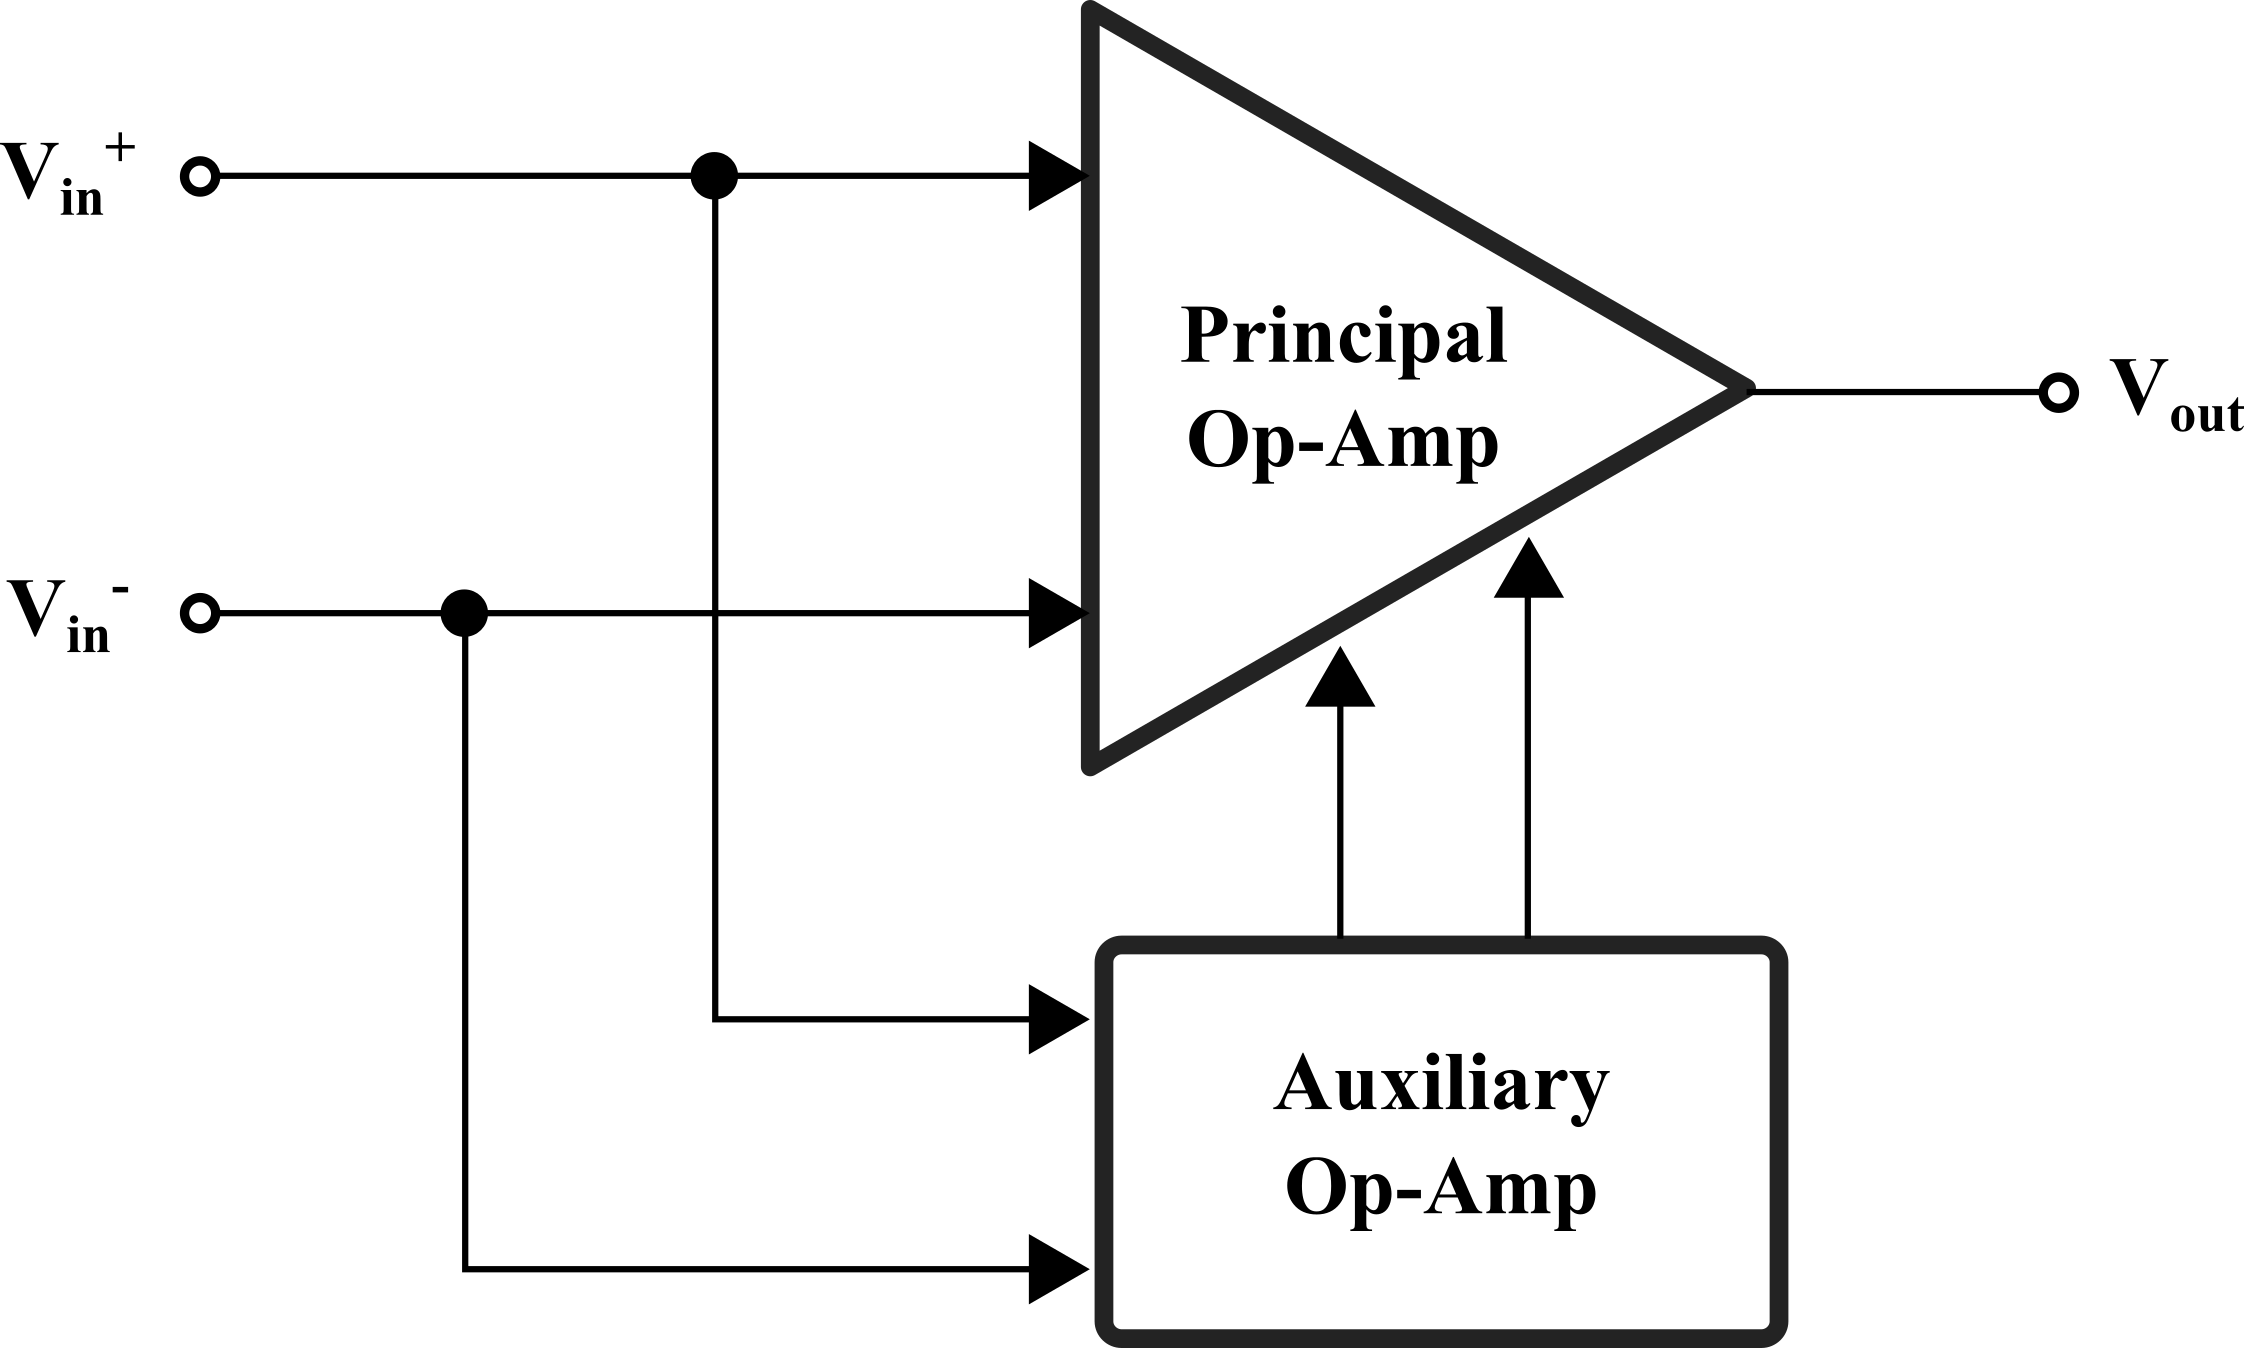
\includegraphics[width=0.6\columnwidth]{Chap05/Figures/block_diagram_gain_enhancement.png}
\caption{Block Diagram of Gain and GBW Enhancement}
\label{BLK_GIN_ENH}
\end{figure}

The circuit level implementation of the architecture is as shown in the Fig. \ref{fig:GIN_ENH_TELE_AMP}. The Auxiliary op-amp is a single stage differential amplifier with diodes as a load. The diode connected loads $M_{a2}$ and $M_{a3}$ in the Auxiliary op-amp are used to bias the current sources $M_5$ and $M_4$ in the principal op-amp respectively as shown in the Fig. \ref{fig:GIN_ENH_TELE_AMP}. With this architecture of the amplifier, all the requirements for the first integrator are fulfilled.

The bias voltages to the current sources in modified architecture for improved swing are fixed as shown in Fig. \ref{TELE_AMP1}. In case of Gain-enhanced telescopic architecture, the bias voltages $v_A$, $v_B$ are generated from auxiliary op-amp and are not constant. These voltages change as the input changes and are applied to the controlled current sources. The signal voltage $v_A$ is applied to transistor $M_4$ and $v_B$ to $M_5$.

\begin{figure}[ht]
\centering
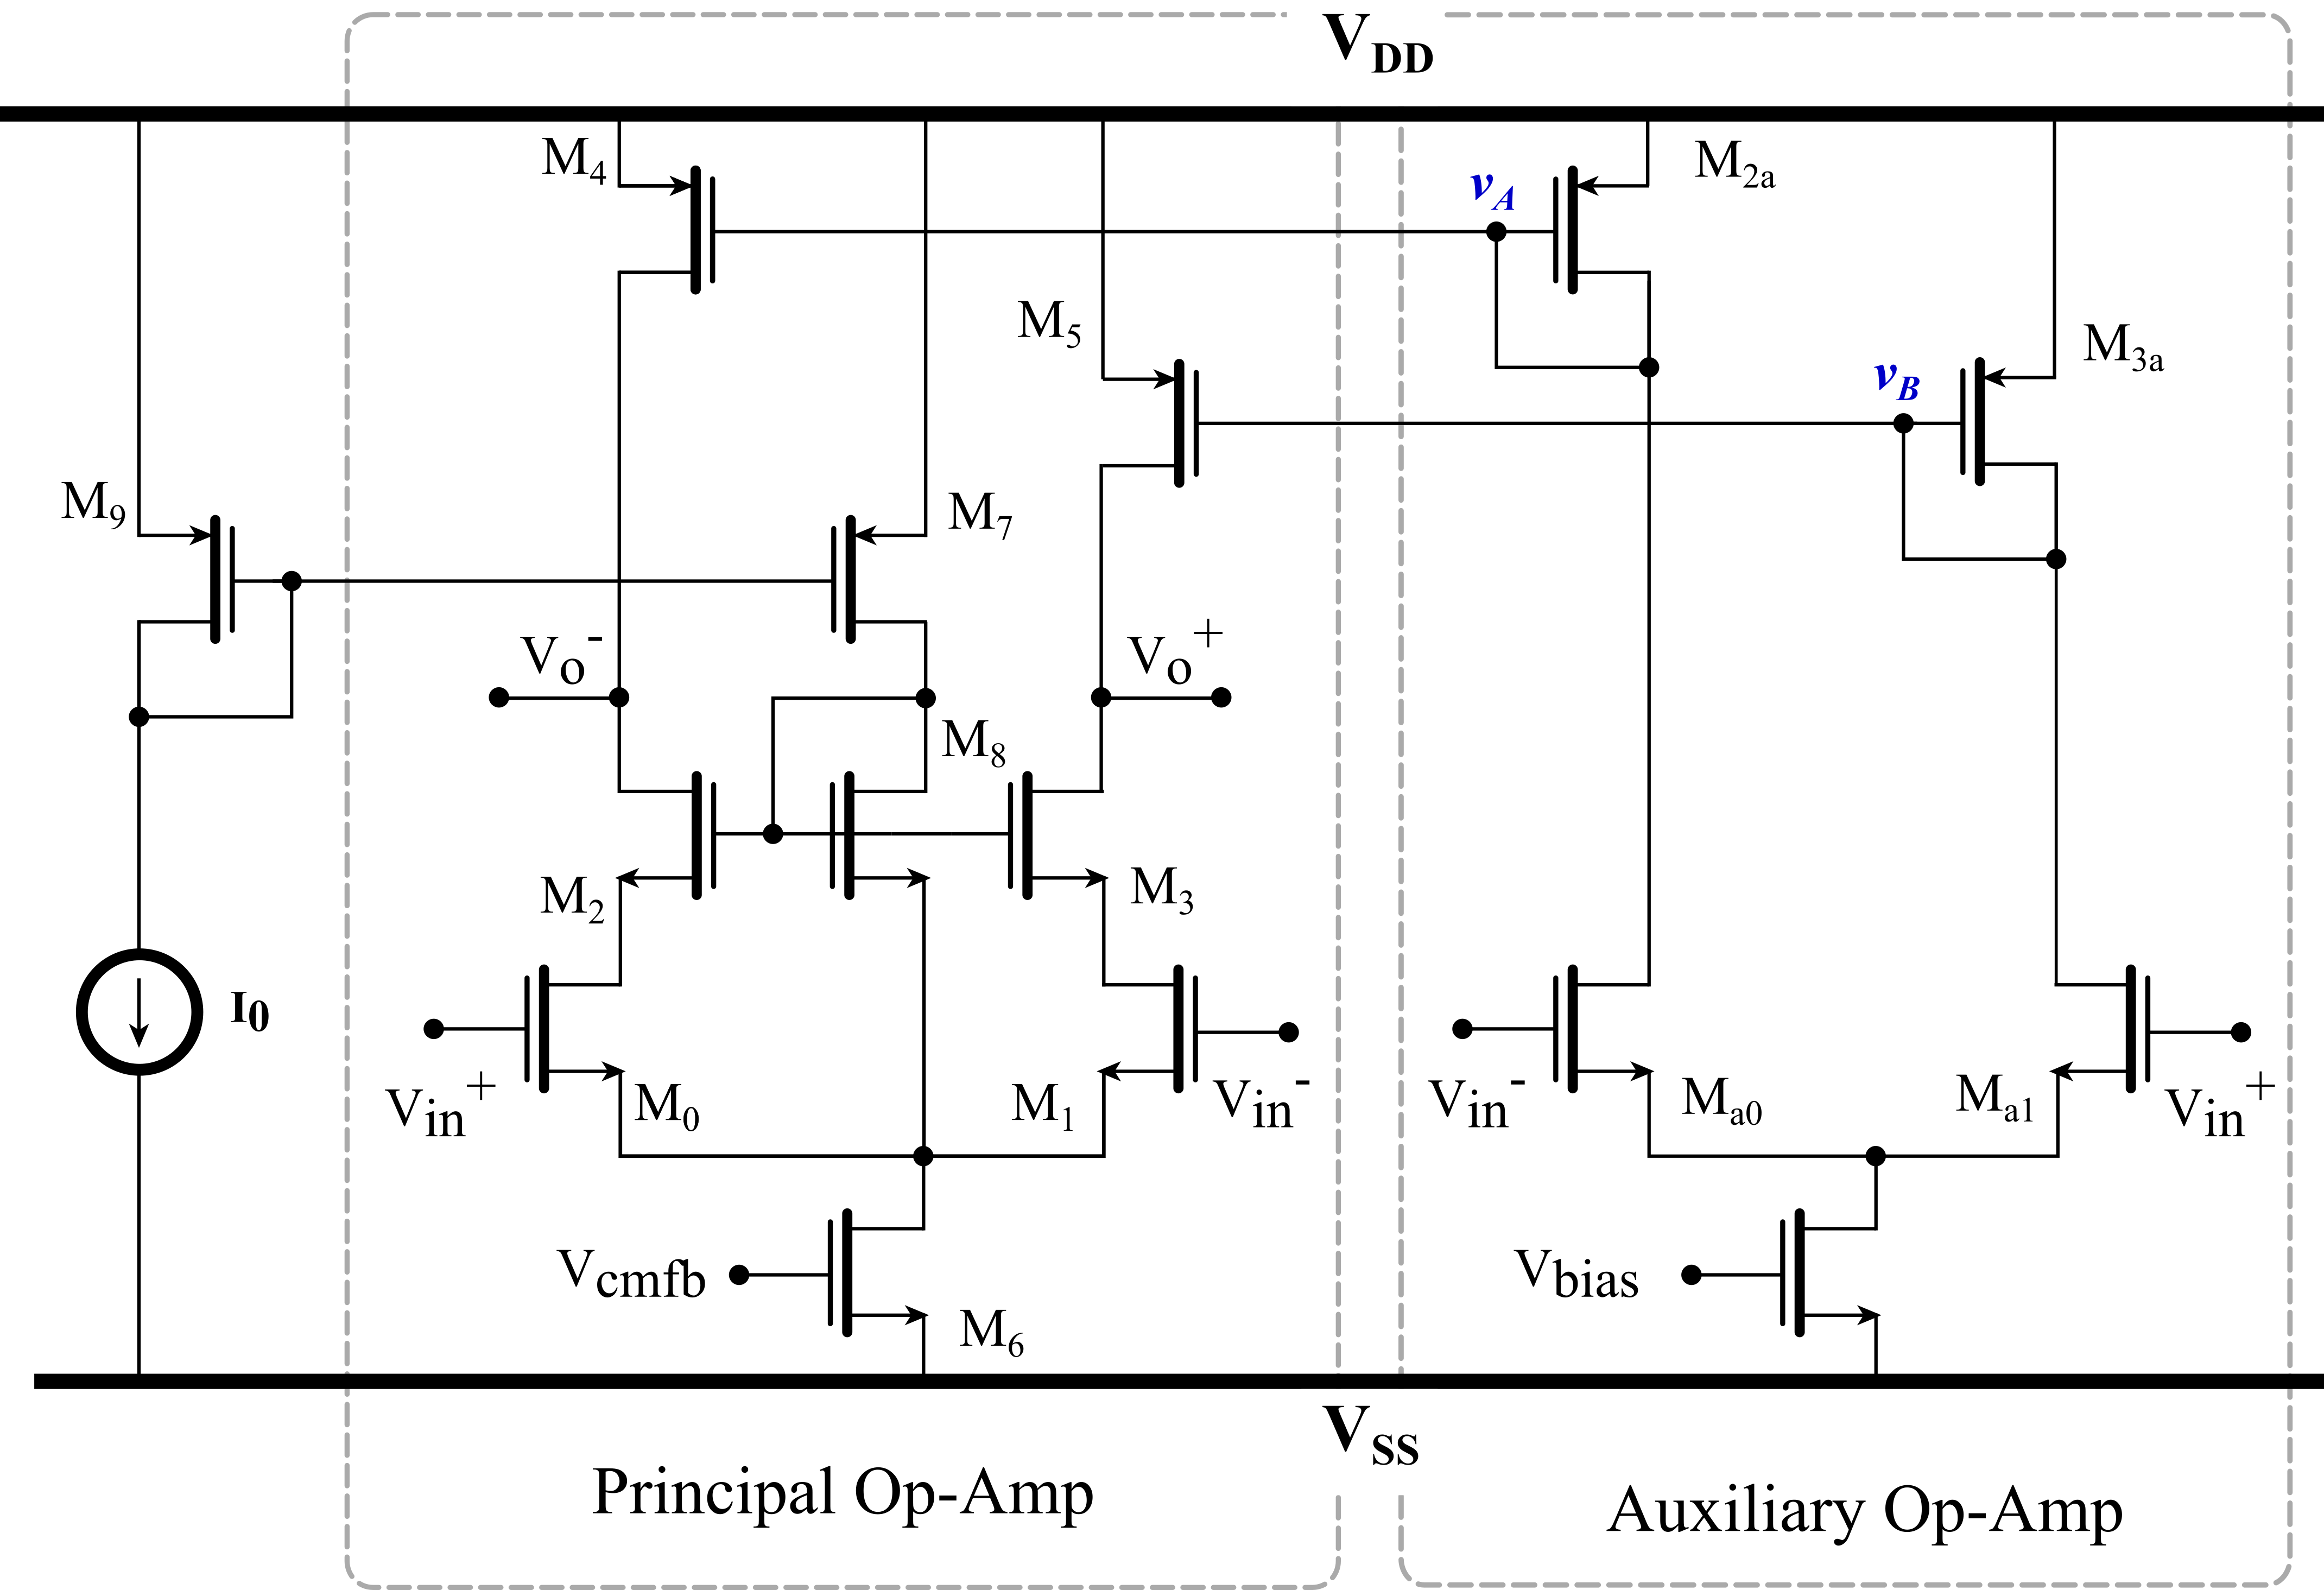
\includegraphics[width=\columnwidth]{Chap05/Figures/gain_enhanced_telescopic.png}
\caption{Gain enhanced Telescopic Amplifier for improved output swing with GBW boost(Common-Mode Feedback circuit not shown)}
\label{fig:GIN_ENH_TELE_AMP}
\end{figure}

Then the expression for $v_A$ and $v_B$ can be given as,
%
\begin{equation}
    v_A = \left(\frac{g_{ma0,a1}}{g_{ma2,a3}}\right) v_{in}^+
\end{equation}
%
%
\begin{equation}
    v_B = \left(\frac{g_{ma0,a1}}{g_{ma2,a3}}\right) v_{in}^-
\end{equation}
%
Now, in the principal op-amp, because of the input signal $v_{in}^+$ and $v_{in}^-$, the current modulation in transistor $M_0$ is $i_0=g_{m0,1}v_{in}^+$ while that in transistor $M_1$ is $i_1=g_{m0,1}v_{in}^-$ that flows through the output resistance, where output resistance is given by,
%
\begin{equation}
    r_{out} = g_{m2,3}r_{O2,3}r_{O0,1}||r_{O4,5}
\end{equation}
%
Furthermore, the non-constant voltages $v_A$ and $v_B$ also causes the further modulation in the output currents through $M_4$ and $M_5$. The expressions of these currents can be given as,
%
\begin{equation}
    i_4 = g_{m4}v_A = g_{m4,5}\left(\frac{g_{ma0,a1}}{g_{ma2,a3}}\right) v_{in}^+
\end{equation}
%
%
\begin{equation}
    i_5 = g_{m5}v_B = g_{m4,5}\left(\frac{g_{ma0,a1}}{g_{ma2,a3}}\right) v_{in}^-
\end{equation}
%

Then the output voltage of the principal op-amp is expressed as,
%
\begin{equation}
    \begin{split}
        v_{out} &= v_{out}^+ - v_{out}^-\\
                &= (i_0+i_4)r_{out} - (i_1+i_5)r_{out}\\
                &= \left\{\left[g_{m0,1}v_{in}^++g_{m4,5}\left(\frac{g_{ma0,a1}}{g_{ma2,a3}}\right) v_{in}^+\right]-\left[g_{m0,1}v_{in}^-+g_{m4,5}\left(\frac{g_{ma0,a1}}{g_{ma2,a3}}\right) v_{in}^-\right]\right\}r_{out}\\
                &=\left(g_{m0,1}+g_{m4,5}\frac{g_{ma0,a1}}{g_{ma2,a3}}\right)r_{out}\left(v_{in}^+ - v_{in}^-\right)
    \end{split}
\end{equation}
%
And therefore, low-frequency gain is represented as,
%
\begin{equation}\label{eq:A0_gain_enhanced}
\begin{split}
    A_0 &= \frac{v_{out}}{v_{in}}=\frac{\left(v_{out}^+ - v_{out}^-\right)}{\left(v_{in}^+ - v_{in}^-\right)}\\ 
        &= \left(g_{m0,1}+g_{m4,5}\frac{g_{ma0,a1}}{g_{ma2,a3}}\right)r_{out}\\
        &=\left(g_{m0,1}+g_{m4,5}\frac{g_{ma0,a1}}{g_{ma2,a3}}\right)\left(g_{m2,3}r_{O2,3}r_{O0,1}||r_{O4,5}\right)
\end{split}
\end{equation}
%
%
\begin{figure}[t]
\centering
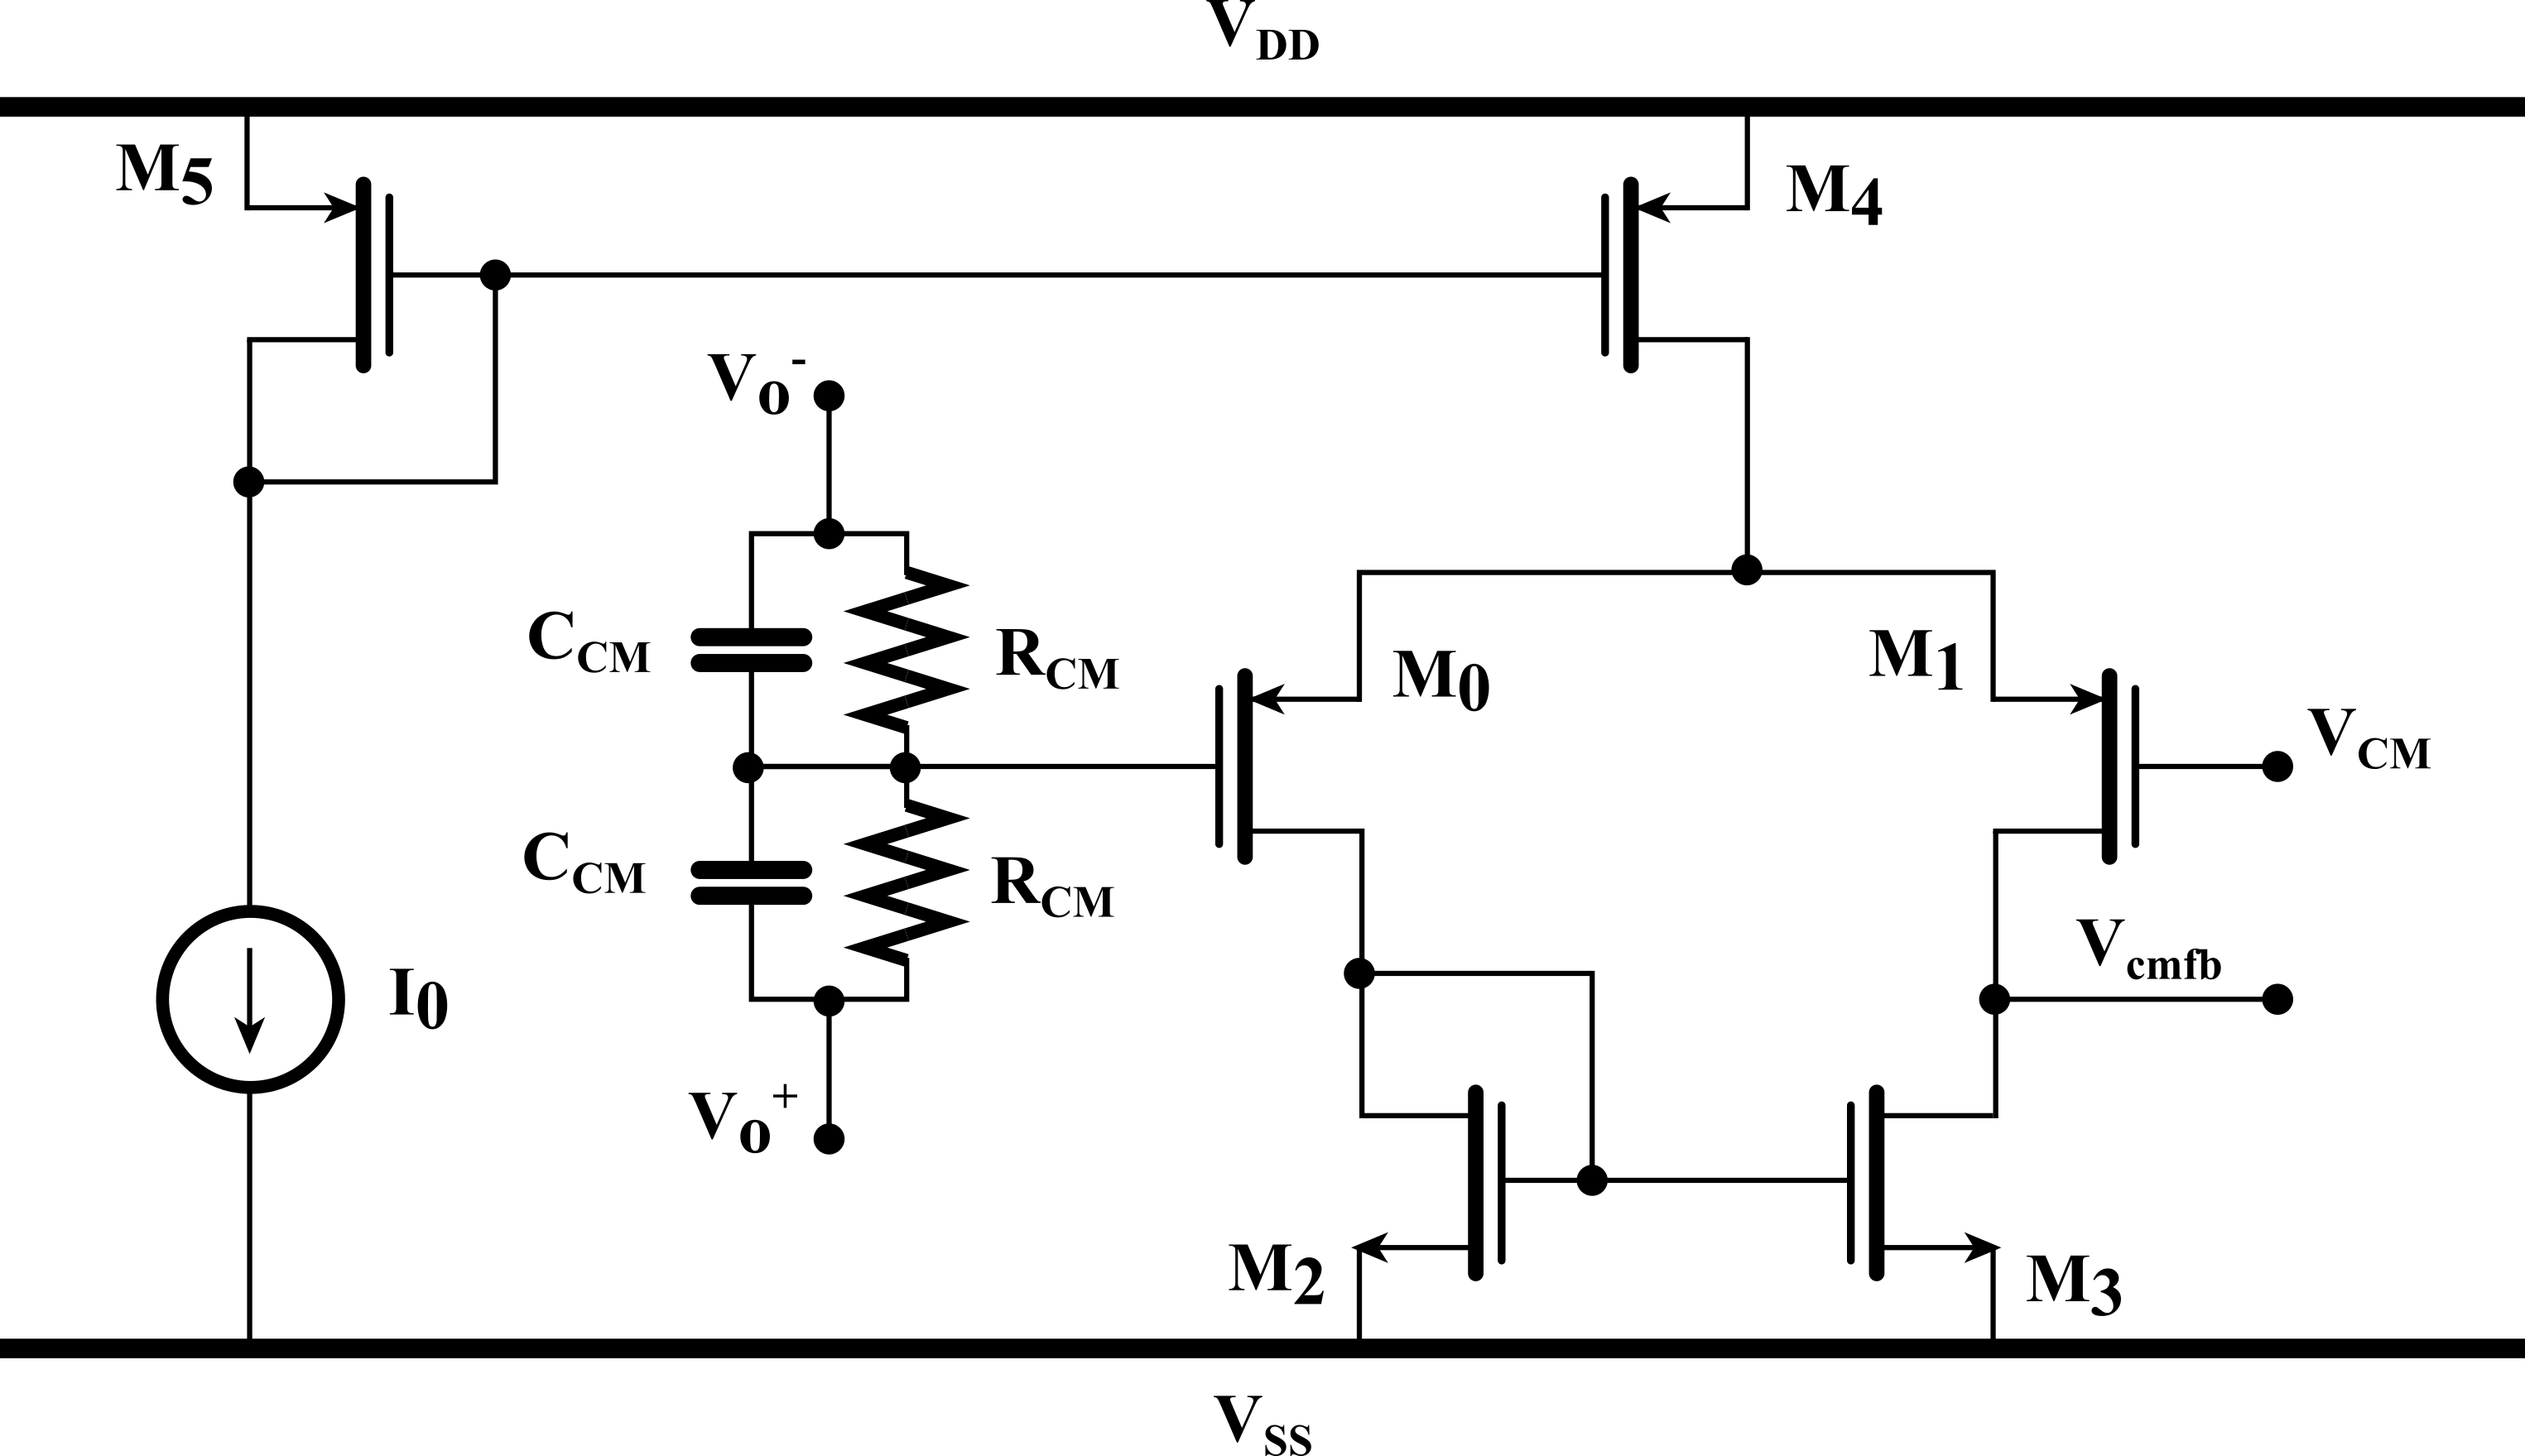
\includegraphics[width=0.8\columnwidth]{Chap05/Figures/common_mode_feedback.png}
\caption{Conventional continuous time Common-Mode Feedback Circuit}
\label{fig:COMMON_MODE}
\end{figure}
%
Eq. (\ref{eq:A_0_swing_improve}) represents the low frequency gain of the modified telescopic amplifier for swing improvement where the transconductance of the structure is $G_m = g_{m0,1}$. While that of the Gain-enhanced telescopic amplifier can be given as, from Eq.(\ref{eq:A0_gain_enhanced}),
%
\begin{equation}
    G_m = g_{m0,1}+g_{m4,5}\frac{g_{ma0,a1}}{g_{ma2,a3}}
\end{equation}
%
It is clear from the equation above that, the scaled transconductance of transistor $M_4$ ($M_5$) is added to the $g_{m0,1}$ boosting it's gain. The GBW also gets raised as a result increase in the transconductance.

%
\begin{figure}[]
\centering
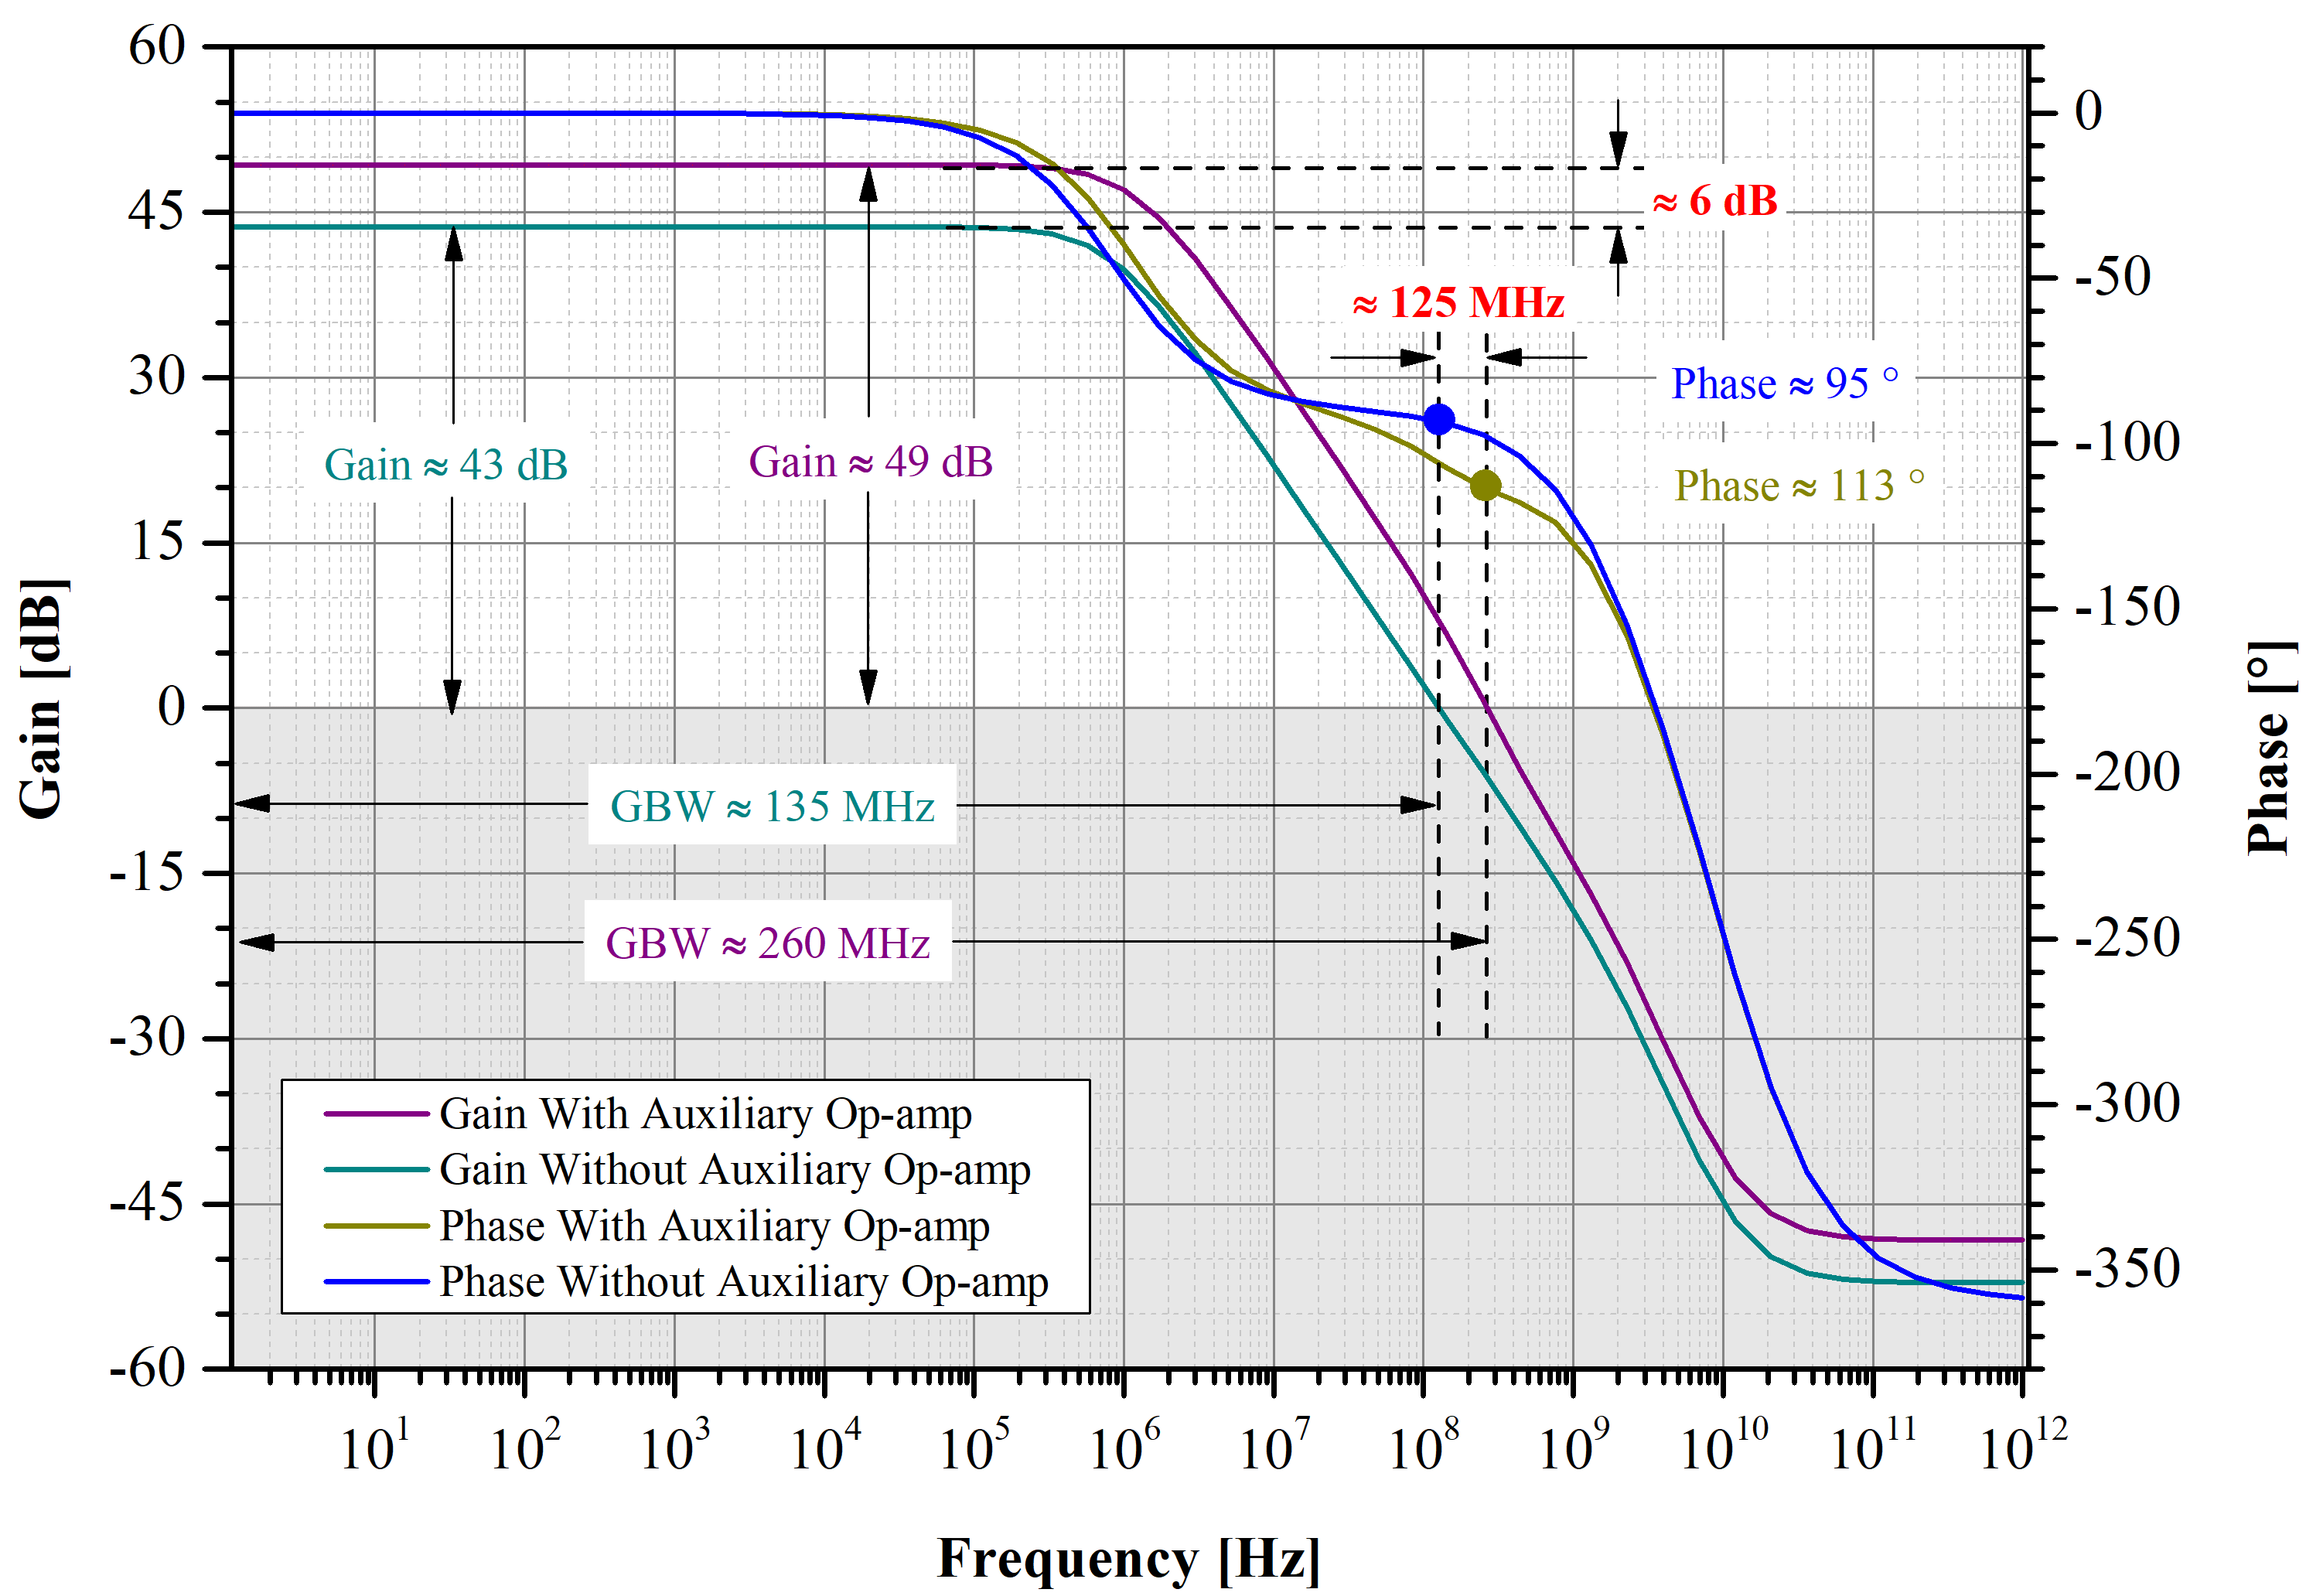
\includegraphics[width=\columnwidth]{Chap05/Figures/gain_gbw_comparison.png}
\caption{Frequency Response comparison between the modified Telescopic amplifier architectures with and without the Auxiliary op-amp for the first integrator}
\label{fig:gain_gbw_comparison}
\end{figure}
%
%
\begin{equation}
\begin{split}
        GBW &= \frac{\left(g_{m0,1}+g_{m4,5}\frac{g_{ma0,a1}}{g_{ma2,a3}}\right)}{2\pi C_L} \\
            &= \left(1+\frac{g_{m4,5}}{g_{m0,1}}\frac{g_{ma0,a1}}{g_{ma2,a3}}\right)\frac{g_{m0,1}}{2\pi C_L}
\end{split}
\end{equation}
%

The Fig.\ref{fig:gain_gbw_comparison} shows the schematic simulation results comparison between the architectures of the modified telescopic amplifiers without auxiliary op-amp (Fig. \ref{TELE_AMP1}) and with auxiliary op-amp (Fig. \ref{fig:GIN_ENH_TELE_AMP}). The gain characteristic and the phase characteristics are plotted as a function of frequency for the modified architecture of telescopic amplifier with and without the auxiliary op-amp. 

In case of the modified architecture of telescopic amplifier for improved swing without auxiliary op-amp, the low frequency gain attained is around 43~dB, gain-bandwidth product is around 135~MHz and the phase margin is 85~° (180-95). While, when an auxiliary op-amp is incorporated to bias the current sources of principal op-amp, the achieved low frequency gain increases to 49~dB, GBW increases to around 260~MHz with phase margin of around 67~°. For the 135~MHz of given GBW, the op-amp architecture without auxiliary op-amp consumes a current of 470~µA, while the op-amp architecture with auxiliary op-amp consumes just 500~µA of current (470~µA in the principal op-amp and 30~µA in the auxiliary op-amp) boosting the gain by 6~dB and GBW by 125~MHz, i.e. there is almost 100\% increase in the gain as well as GBW with just nominal amount of extra current consumption of just 6-7\% (30~µA).
%
\begin{figure}[h!]
\centering
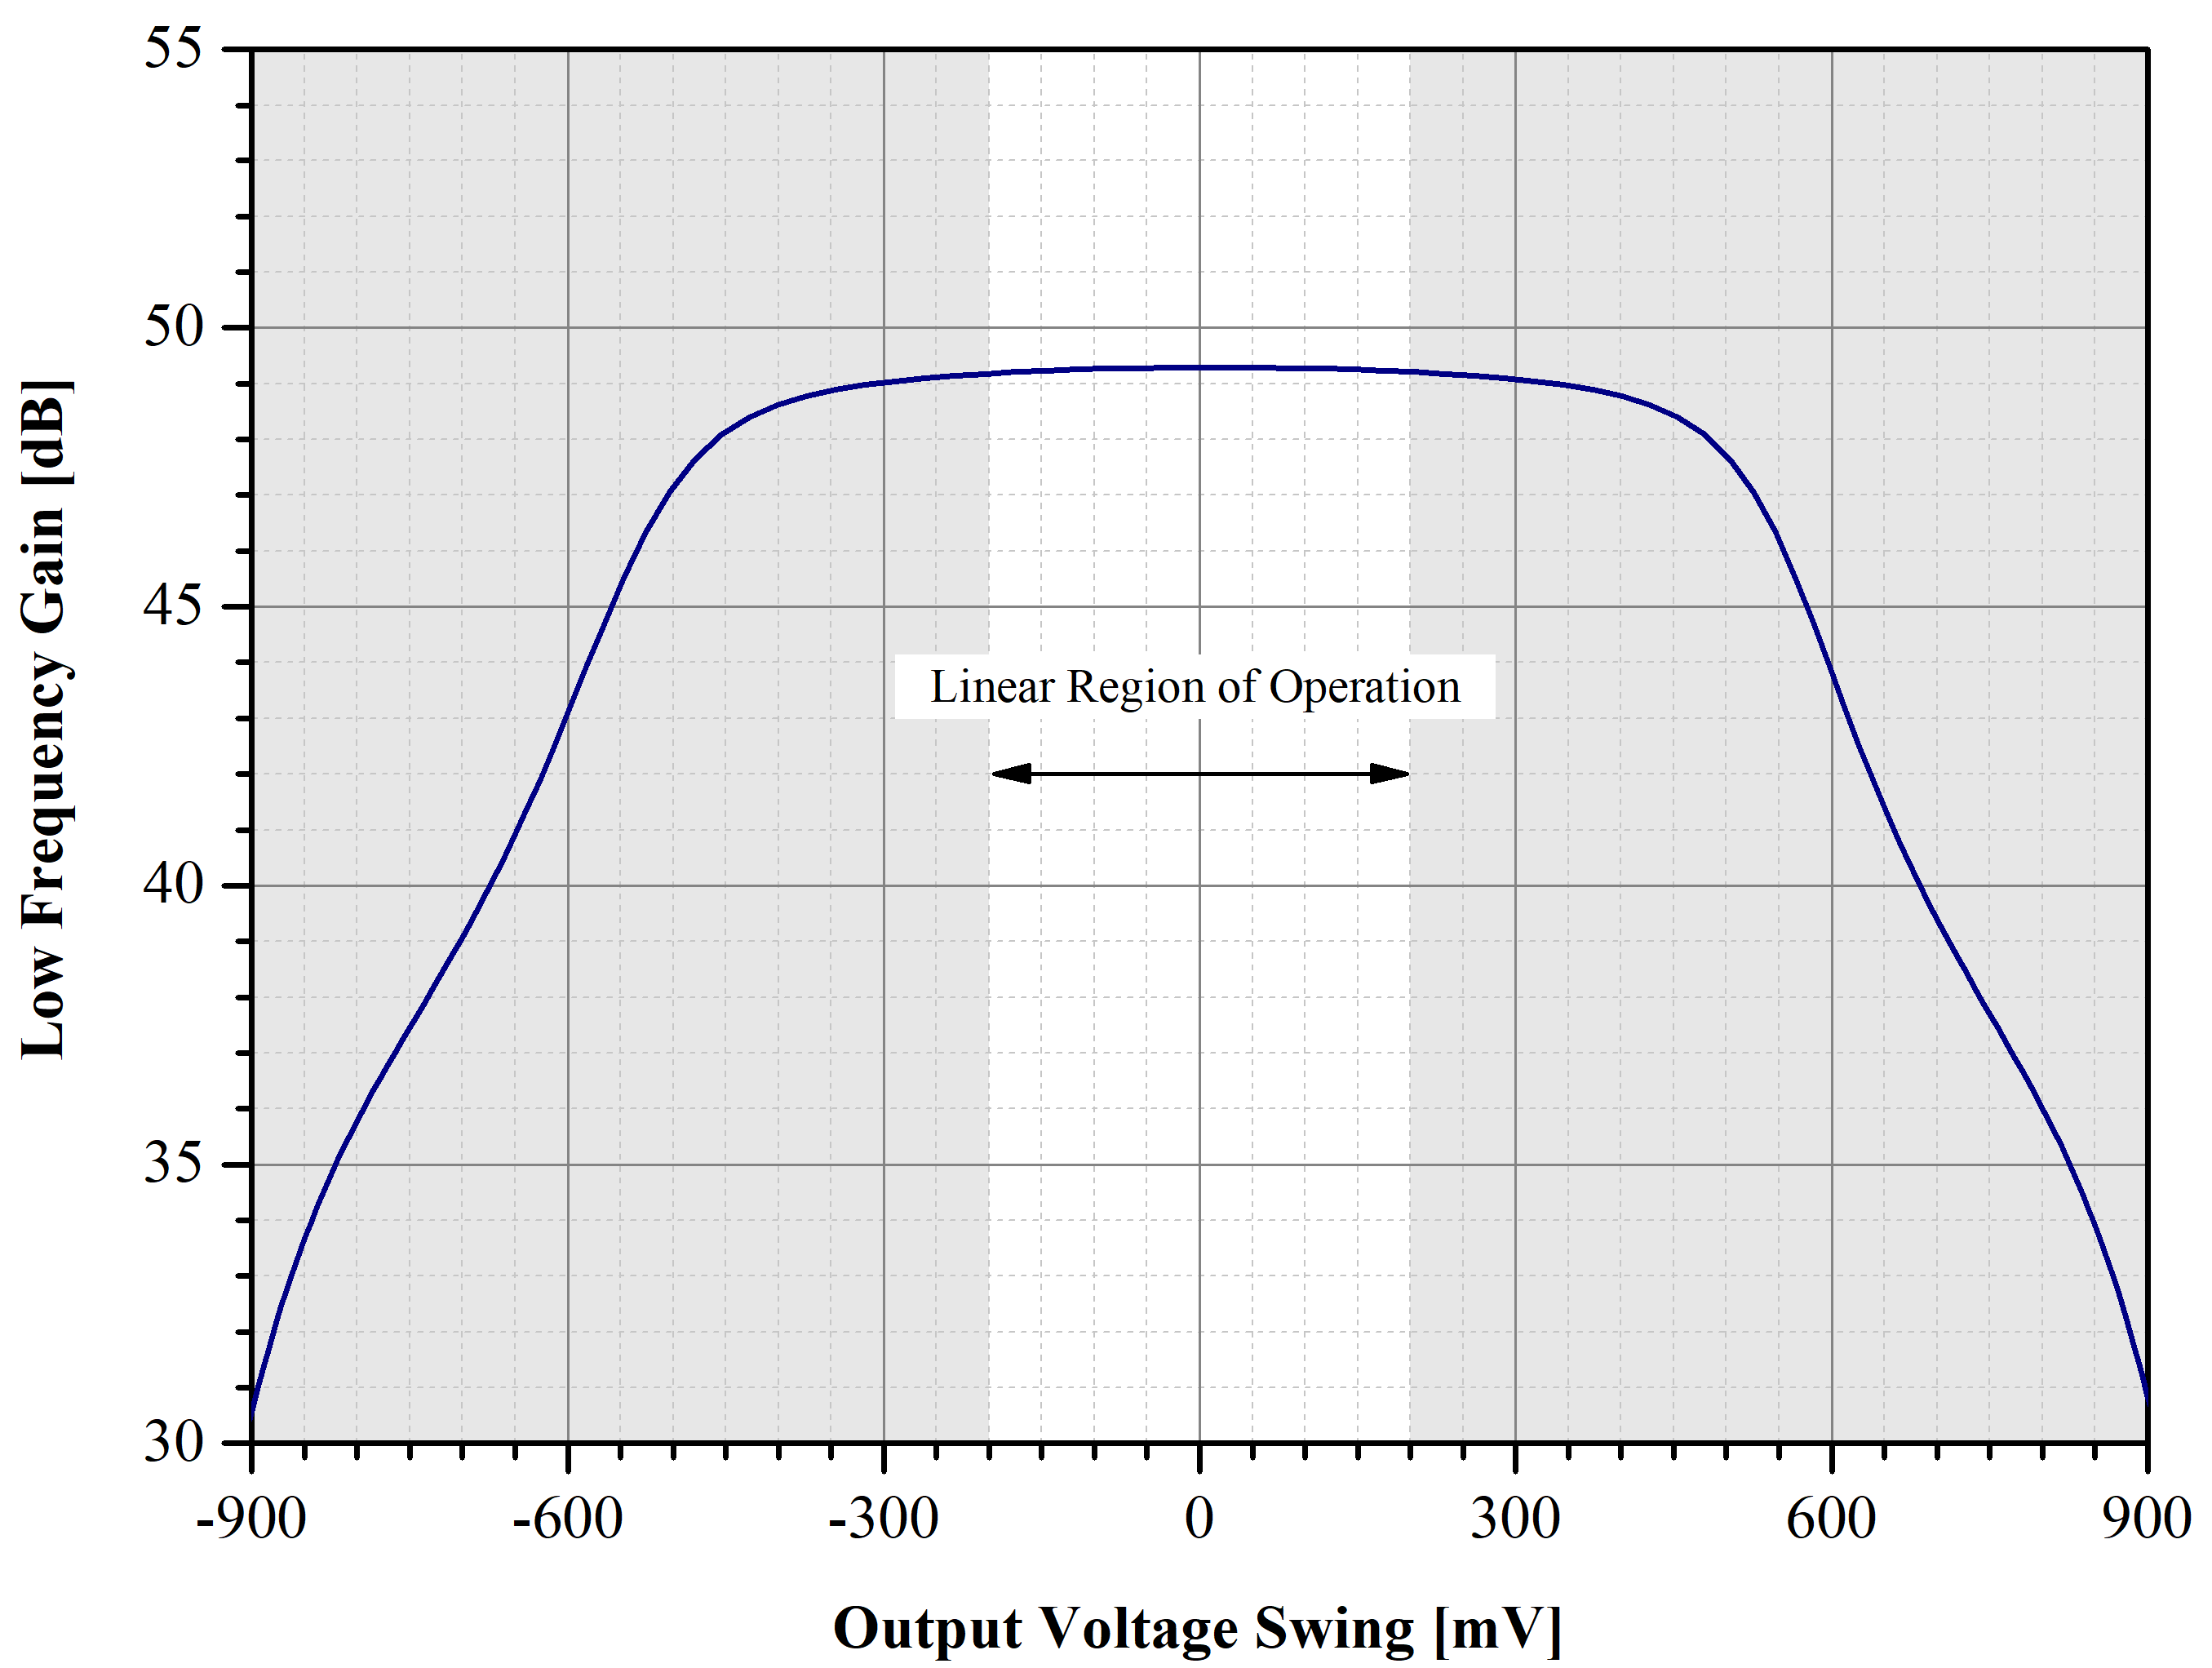
\includegraphics[width=0.9\columnwidth]{Chap05/Figures/gain_vs_swing.png}
\caption{Output swing of the Op-amp Vs low frequency gain}
\label{fig:gain_vs_swing}
\end{figure}
%

Next, the analysis of output voltage swing of the op-amp architecture has also been done having considered the constant voltage gain region. The low frequency gain is plotted as a function of differential output voltage swing as shown in Fig. \ref{fig:gain_vs_swing}. It is clear from the figure that the low frequency gain is around 50~dB at 0~mV differential output voltage and remains constant for output voltage from -300~mV to +300~mV exhibiting the swing of 600~mV deferentially.
% Please add the following required packages to your document preamble:
% \usepackage{multirow}
\begin{table}[]
\centering
\begin{tabular}{c|c|c|c}
\Xhline{4\arrayrulewidth}
\multirow{2}{*}{\textbf{Transistor}} & \textbf{First Op-amp} & \textbf{Second Op-amp} &        \\ \cline{2-3} 
                            & W (\textmu m)  & W (\textmu m)  & L (\textmu m) \\ \hline
M\textsubscript{0,1}                        & 60      & 40      & 0.4    \\ 
M\textsubscript{2,3}                        & 45      & 30      & 0.4    \\ 
M\textsubscript{4,5}                        & 75      & 50      & 0.4    \\ 
M\textsubscript{6}                          & 120     & 75      & 0.4    \\ 
M\textsubscript{7}                          & 5       & 5       & 0.4    \\ 
M\textsubscript{8}                          & 5       & 5       & 2.0      \\ \hline
M\textsubscript{a0,a1}                      & 4       & 4       & 0.4    \\ 
M\textsubscript{a2,a3}                      & 6       & 6       & 0.4    \\ 
M\textsubscript{a4}                         & 8       & 8       & 0.4    \\ \Xhline{4\arrayrulewidth}
\end{tabular}
\caption{Transistor sizes in the Op-amps in the first and second integrator}
\label{tab:trans_size}
\end{table}

\subsection{Op-Amp for the Second Integrator:}
Similar way the load for the second integrator can also be estimated in a phase where it has maximum amount of load which is again the integrating phase in this case. The second integrator in the feedforward and in the integrating phase appears as shown in Fig. \ref{INT2_INTPHS}. Then, from the figure, the expression for load and the feedback factor for the second integrator is pronounced in Eq. \ref{CL2} and \ref{BETA2} respectively.
\begin{figure}[h]
\centering
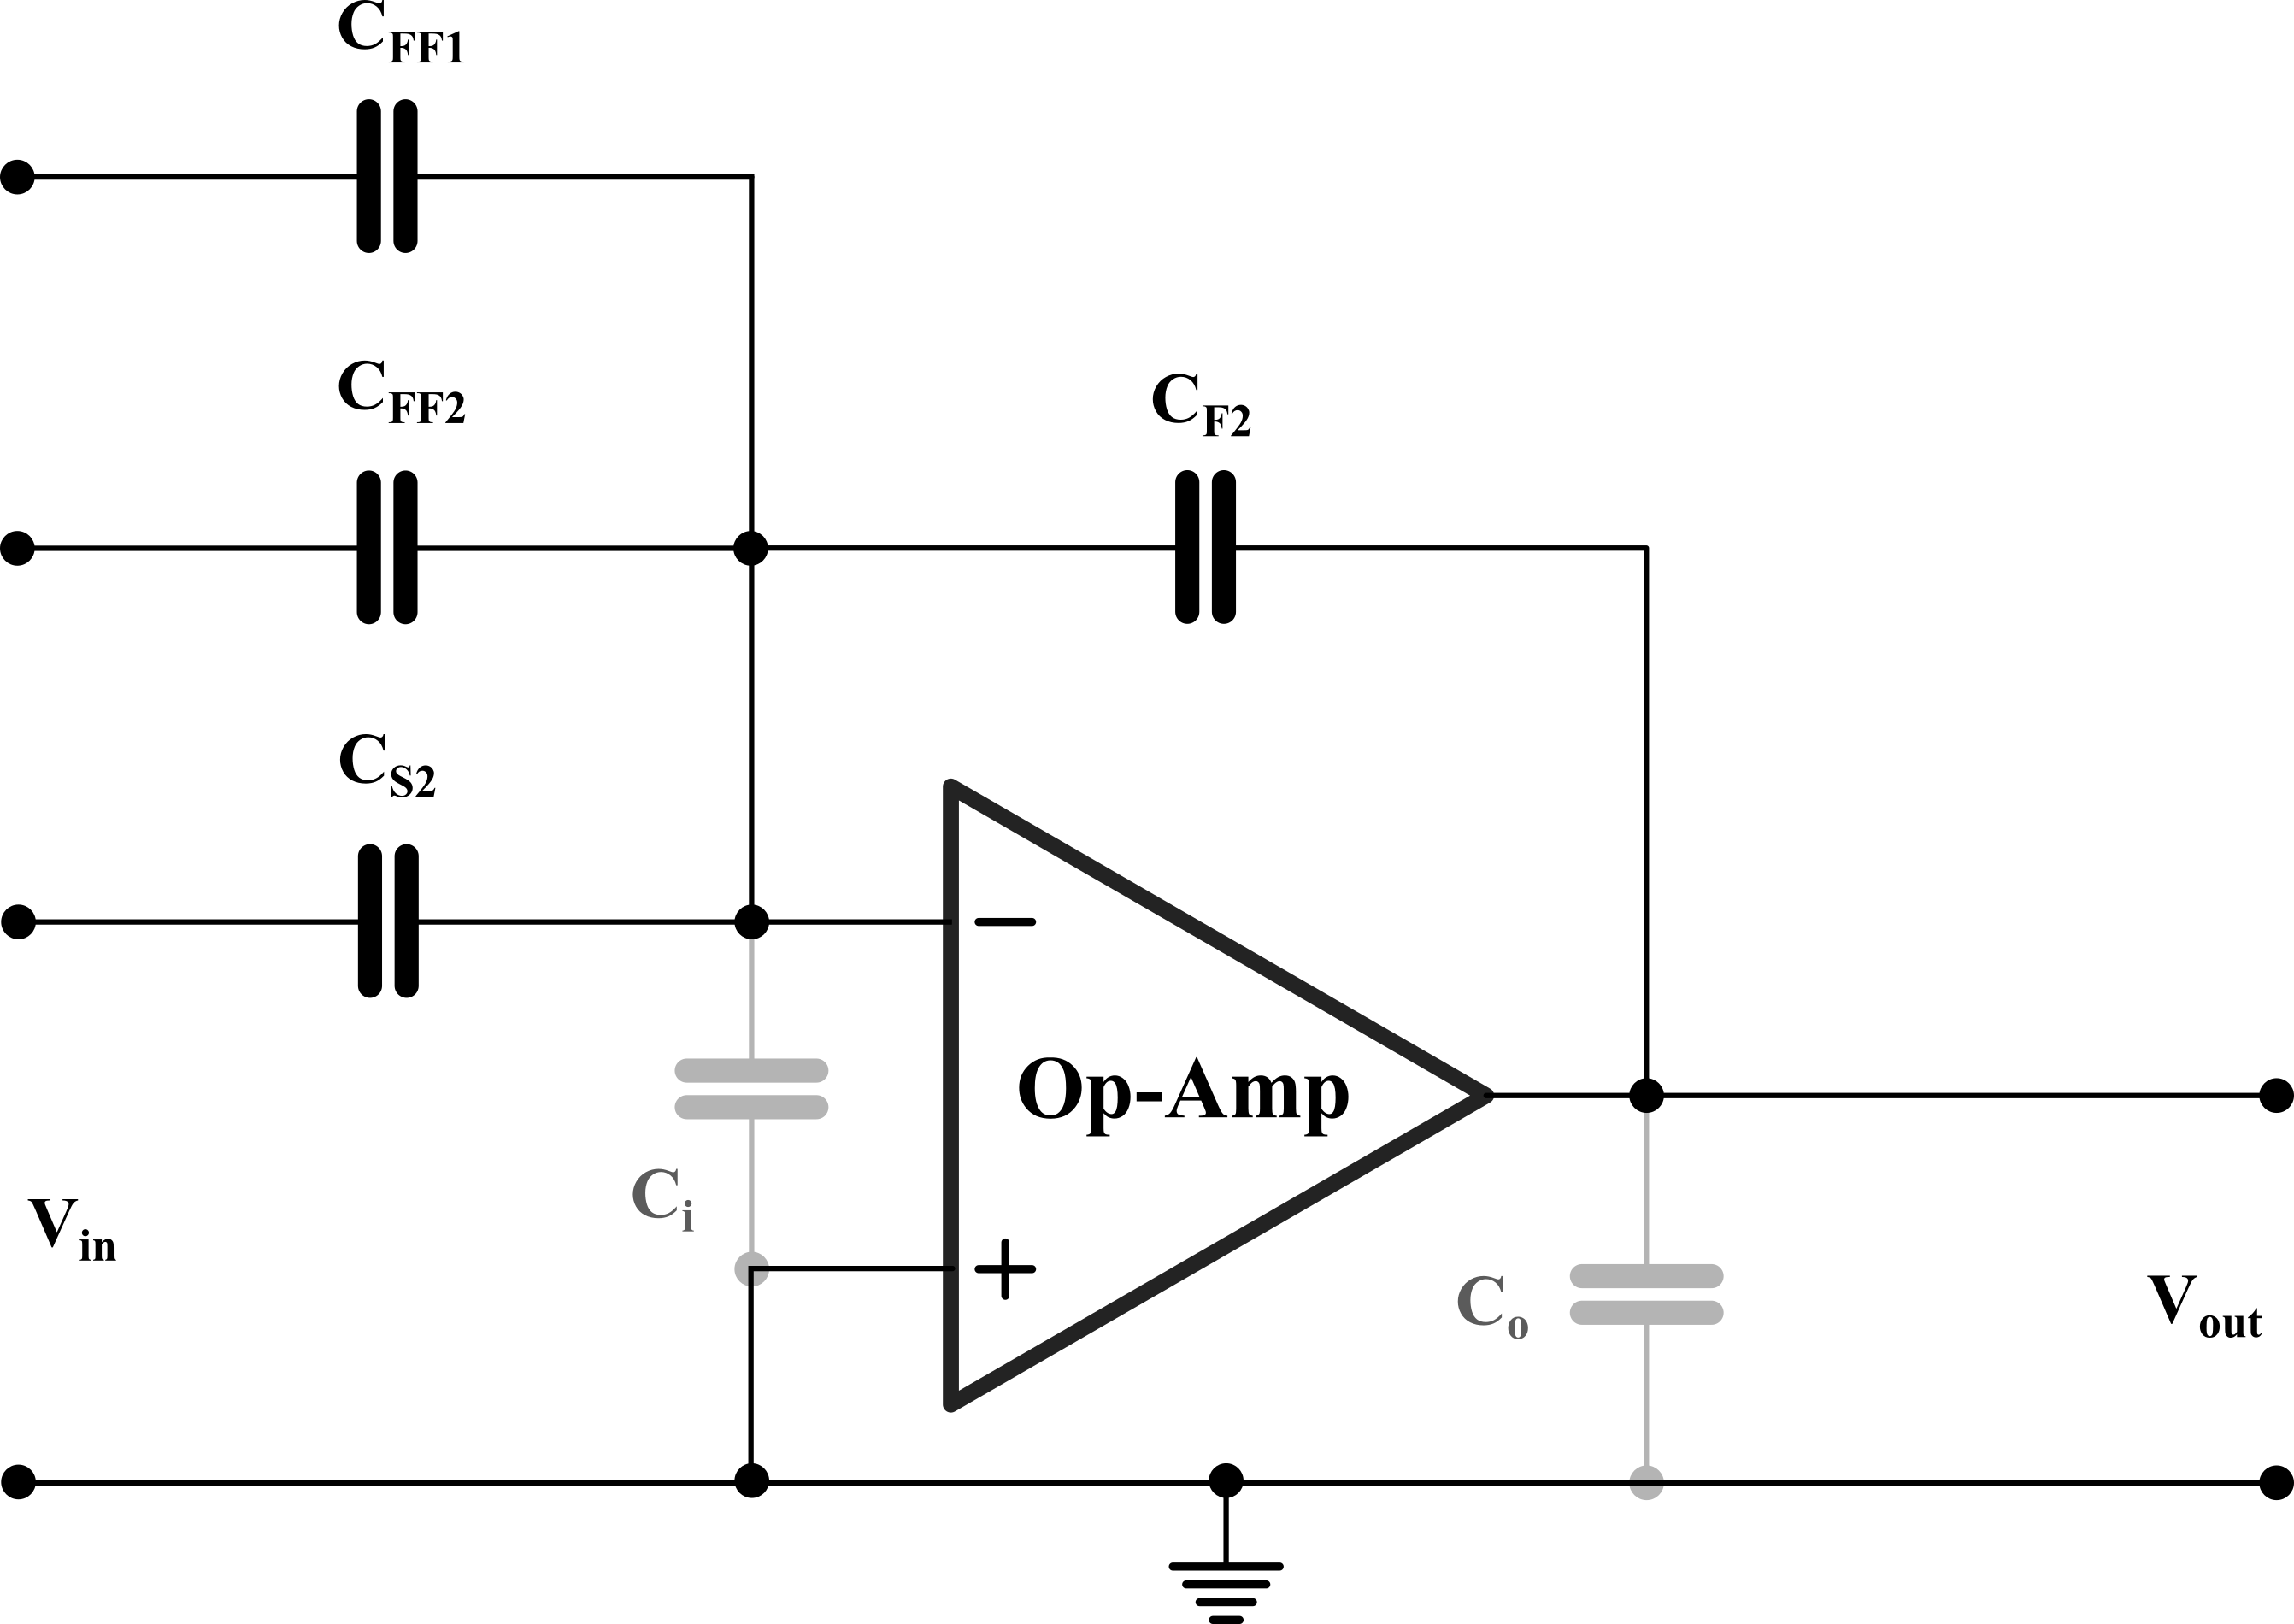
\includegraphics[width=0.6\columnwidth]{Chap05/Figures/integrator2.png}
\caption{Single Ended representation of the second Integrator in the integrating phase}
\label{INT2_INTPHS}
\end{figure}
\begin{equation}
    C_{L2}=\frac{C_{F2}\left(C_{S2}+C_{FF1}+C_{FF2}+C_{i}\right)}{C_{F2}+C_{S2}+C_{FF1}+C_{FF2}+C_{i}}+C_{o}
    \label{CL2}
\end{equation}
\begin{equation}
    \beta_{2}=\frac{C_{F2}}{C_{F2}+C_{S2}+C_{FF1}+C_{FF2}+C_{i}}
    \label{BETA2}
\end{equation}

However, in the architecture of Op-amp developed (Fig. \ref{fig:GIN_ENH_TELE_AMP}), there are four transistors stacked from positive to negative rail, while the output voltage swing requirement is 1.2~V with GBW of around 200~MHz (considering PVT variations). In order to achieve such a high GBW (even with the modified structure), it is necessary to bias the transistors in the strong inversion region, and thus at higher overdrive voltage. With these restrictions, it is quite difficult to achieve the given voltage swing. Therefore, the option is to change the coefficients of the three inputs to the second integrator by proper amount so as to accommodate the resulting signal within the voltage swing of the op-amp. Previously, the values of capacitors $C_{FF1}$, $C_{F2}$ and $C_{S2}$ were 400~fF and that of $C_{FF2}$ was 800~fF setting the coefficients, $a_2=1$, $b_1=1$ and $b_2=2$, where $a_2=\frac{C_{S2}}{C_{F2}}$, $b_1=\frac{C_{FF1}}{C_{F2}}$, $b_2=\frac{C_{FF2}}{C_{F2}}$ and as discussed, these coefficients were leading the signal swing to 1.2~V. A good scale-down coefficient could be 4 which results swing of (1.2V/4=) 300~mV and it is known that the op-amp developed for the first integrator already exhibit the same output swing, consequently which can be employed also for the op-amp in the second integrator. To do so, all the coefficients $a_2$, $b_1$ must be set to $\frac{1}{4}$ and $a_2$ must be set to $\frac{1}{2}$ which can simply be done by reducing the sizes of the input capacitors by 4. Then, final values of the capacitors are, $C_{FF1}=100~fF$, $C_{FF2}=200~fF$, $C_{S2}=100~fF$ and $C_{F2}=400~fF$.


Even in this case, the presumption for the parasitic capacitance at the virtual ground node ($C_{i}$) and the output node ($C_{o}$) is made to be around $100\ fF$. The overall load capacitor ($C_{L2}$) and the feedback factor ($\beta_2$) are computed with the help of Eq. \ref{CL2} and Eq. \ref{BETA2} and are found to be around $300~fF$ and $0.45$ respectively. Eventually similar architecture is used for the op-amp in the second integrator as that used for op-amp in the first (Fig. \ref{fig:GIN_ENH_TELE_AMP}) for the specifications, gain of $50~dB$, GBW of $200~MHz$ and SR of $200~V/\mu s$ for estimated load and $\beta$. The expressions for loop gain and loop GBW is then expressed as,
%
\begin{equation}
    Loop\ GBW = \beta_2 \ GBW_{OL} = \beta_2 \frac{g_m}{2\pi C_{L2}}
\end{equation}
%
%
\begin{equation}
    Loop\ Gain = \beta_2\ A_{OL}
\end{equation}
%
% %
% \begin{figure}[h]
% \centering
% 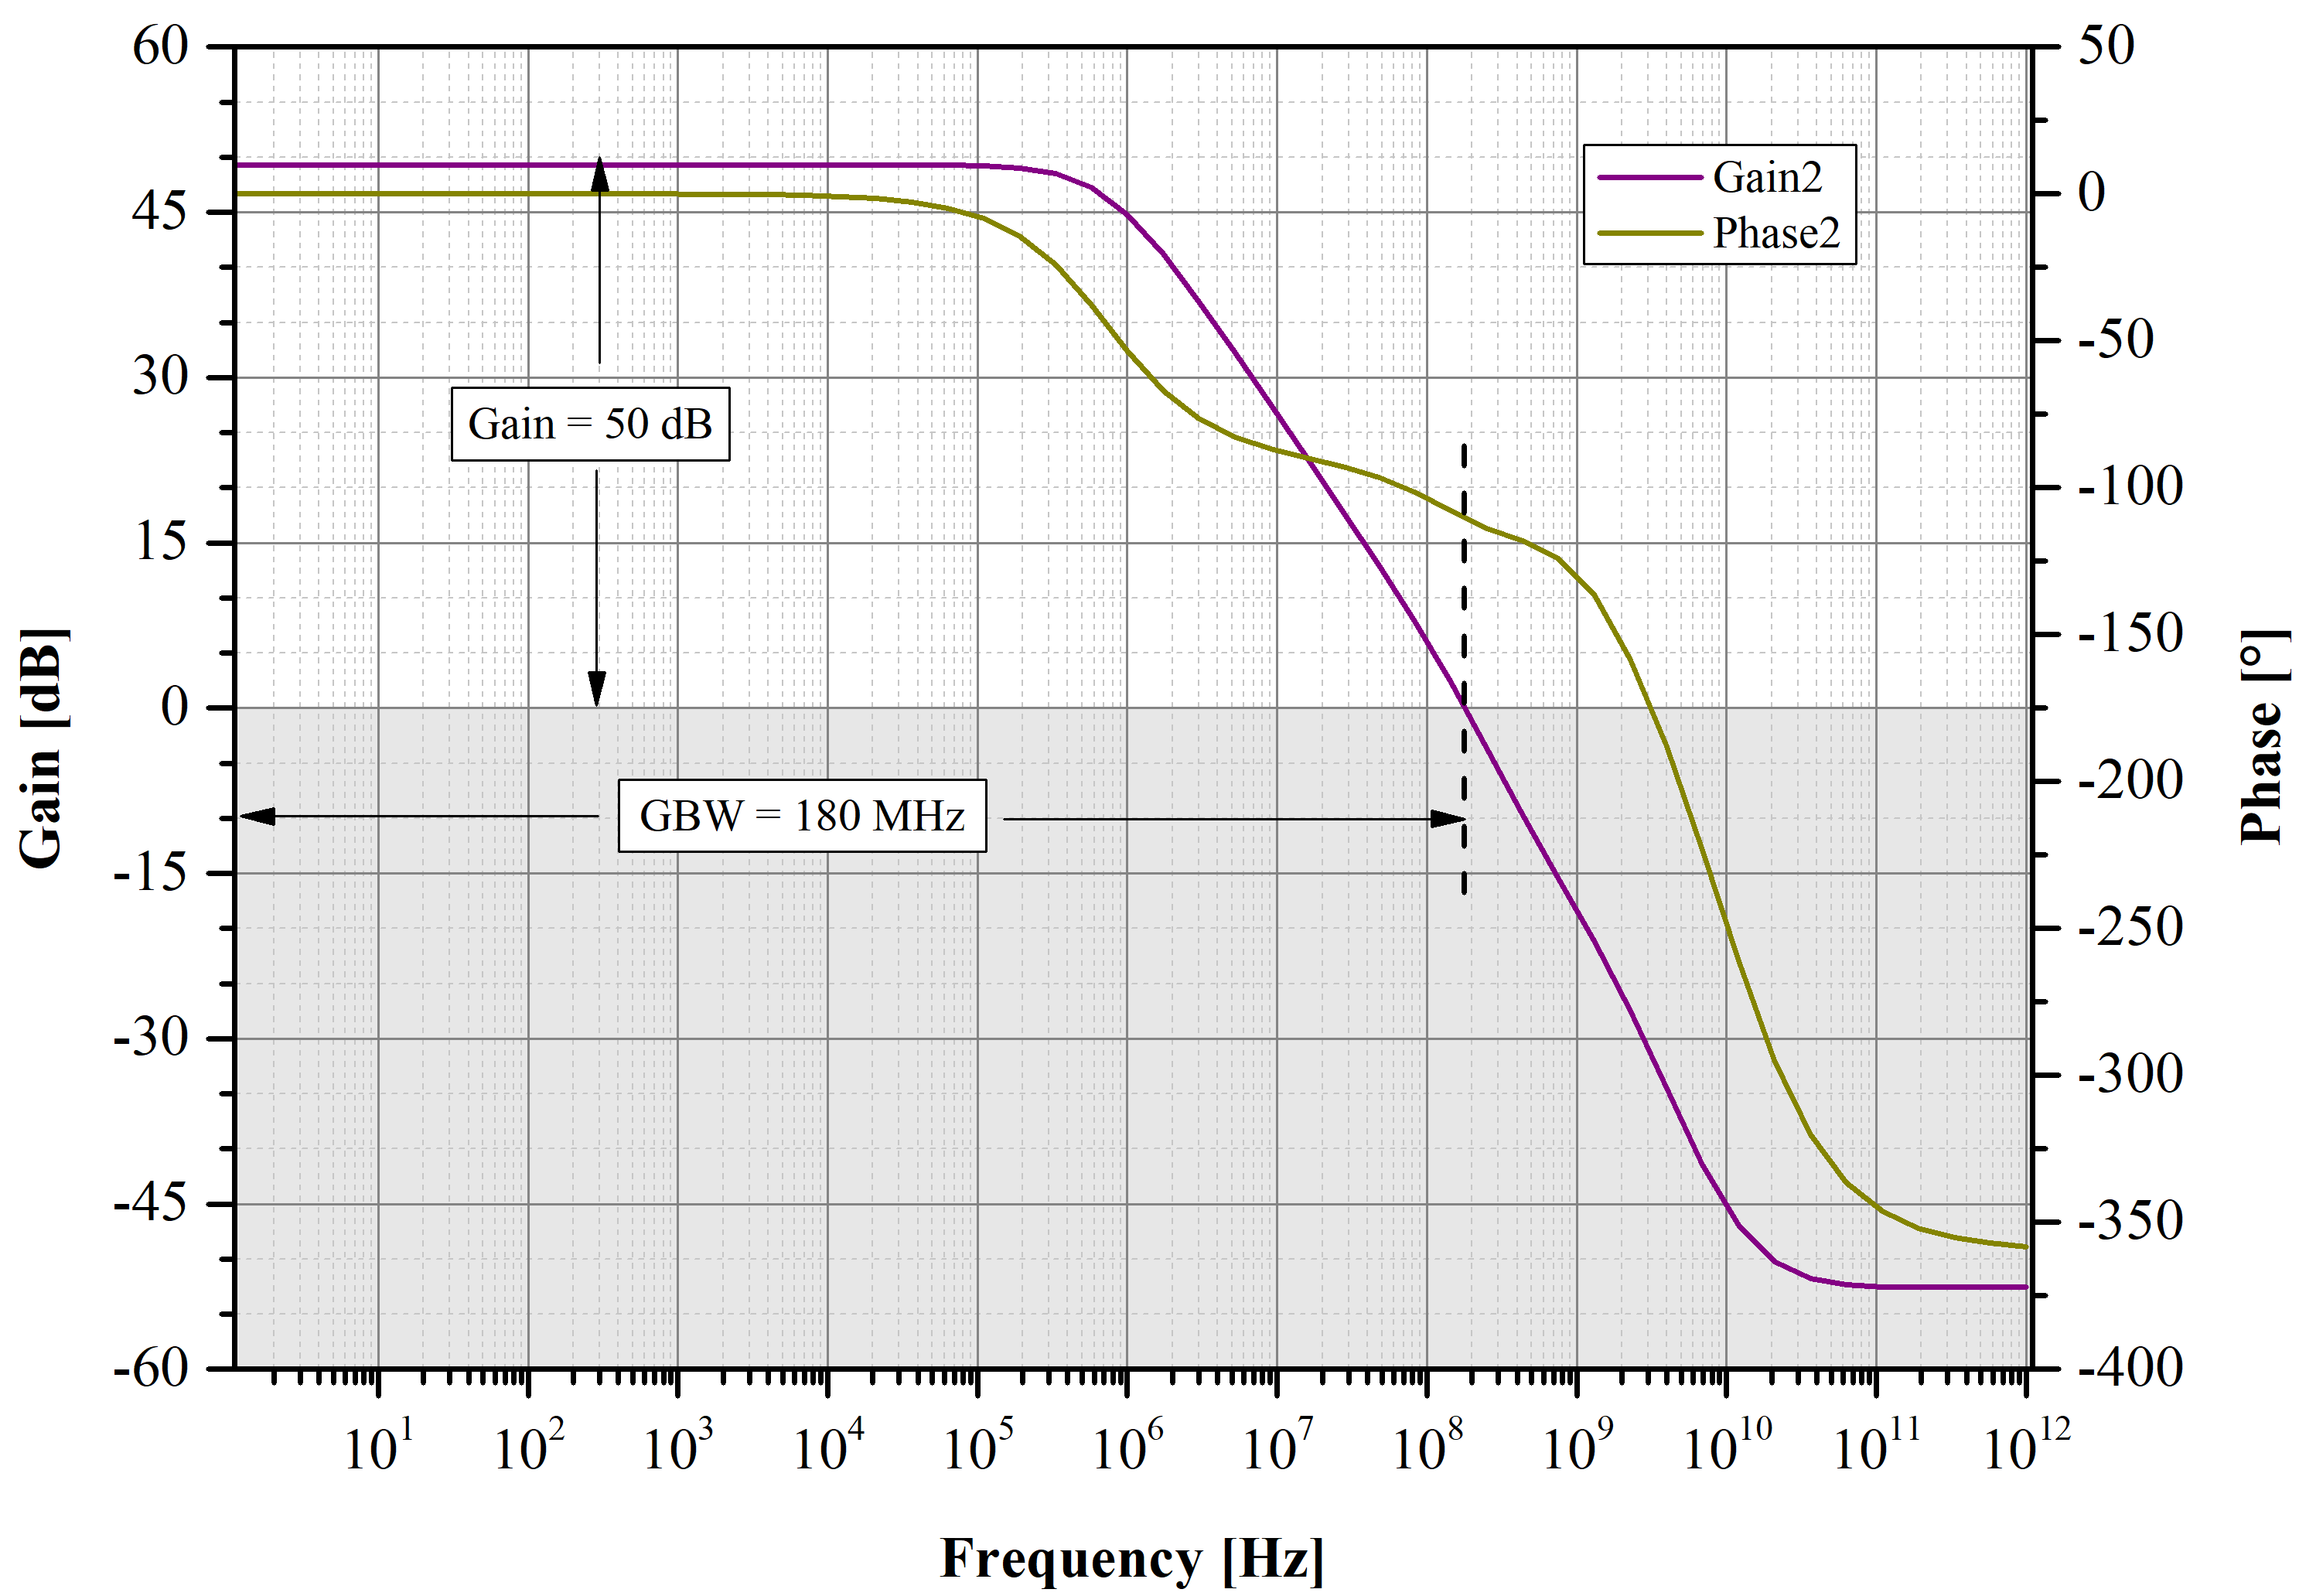
\includegraphics[width=0.85\columnwidth]{Chap05/Figures/gain2_phase2_vs_freq.png}
% \caption{Frequency Response of the Op-amp used in the Second integrator}
% \label{fig:gain2_phase2}
% \end{figure}
% %
\section{Quantizer}
A quantizer block in the IADC to be employed is of the resolution of 3-bit i.e. 8 levels as extracted from the simulink simulations. Therefore the total number of comparators needed to build a quantizer are $(2^{N_{SD}}-1)$ i.e. 7. Each comparator has a different threshold voltage where these thresholds are generated from the switched capacitor arrangement. 

\subsection{Threshold Generator}
The simplest solution to generate the thresholds of the comparator is a resistive ladder as shown in Fig.\ref{fig:res_lad}. The differential threshold is the difference of the voltage generated by resistive dividers at that node, e.g. the threshold $V_{1}$ can be given as,
%
\begin{equation}
    \begin{split}
        V_1 &= \frac{\left(\frac{9R}{2}\right)}{7R}\left(V_{refp}-V_{refn}\right)-\frac{\left(\frac{5R}{2}\right)}{7R}\left(V_{refp}-V_{refn}\right)\\
            &=\frac{4}{14}\left(V_{refp}-V_{refn}\right)
    \end{split}
\end{equation}
%
However, the resistors stacked between the positive and negative references tend to draw considerable amount of current, which then has to be taken into account while budgeting the power. The power consumption in the this threshold generator can be minimized by increasing the unit resistance value. 
%
\begin{figure}[h]
\centering
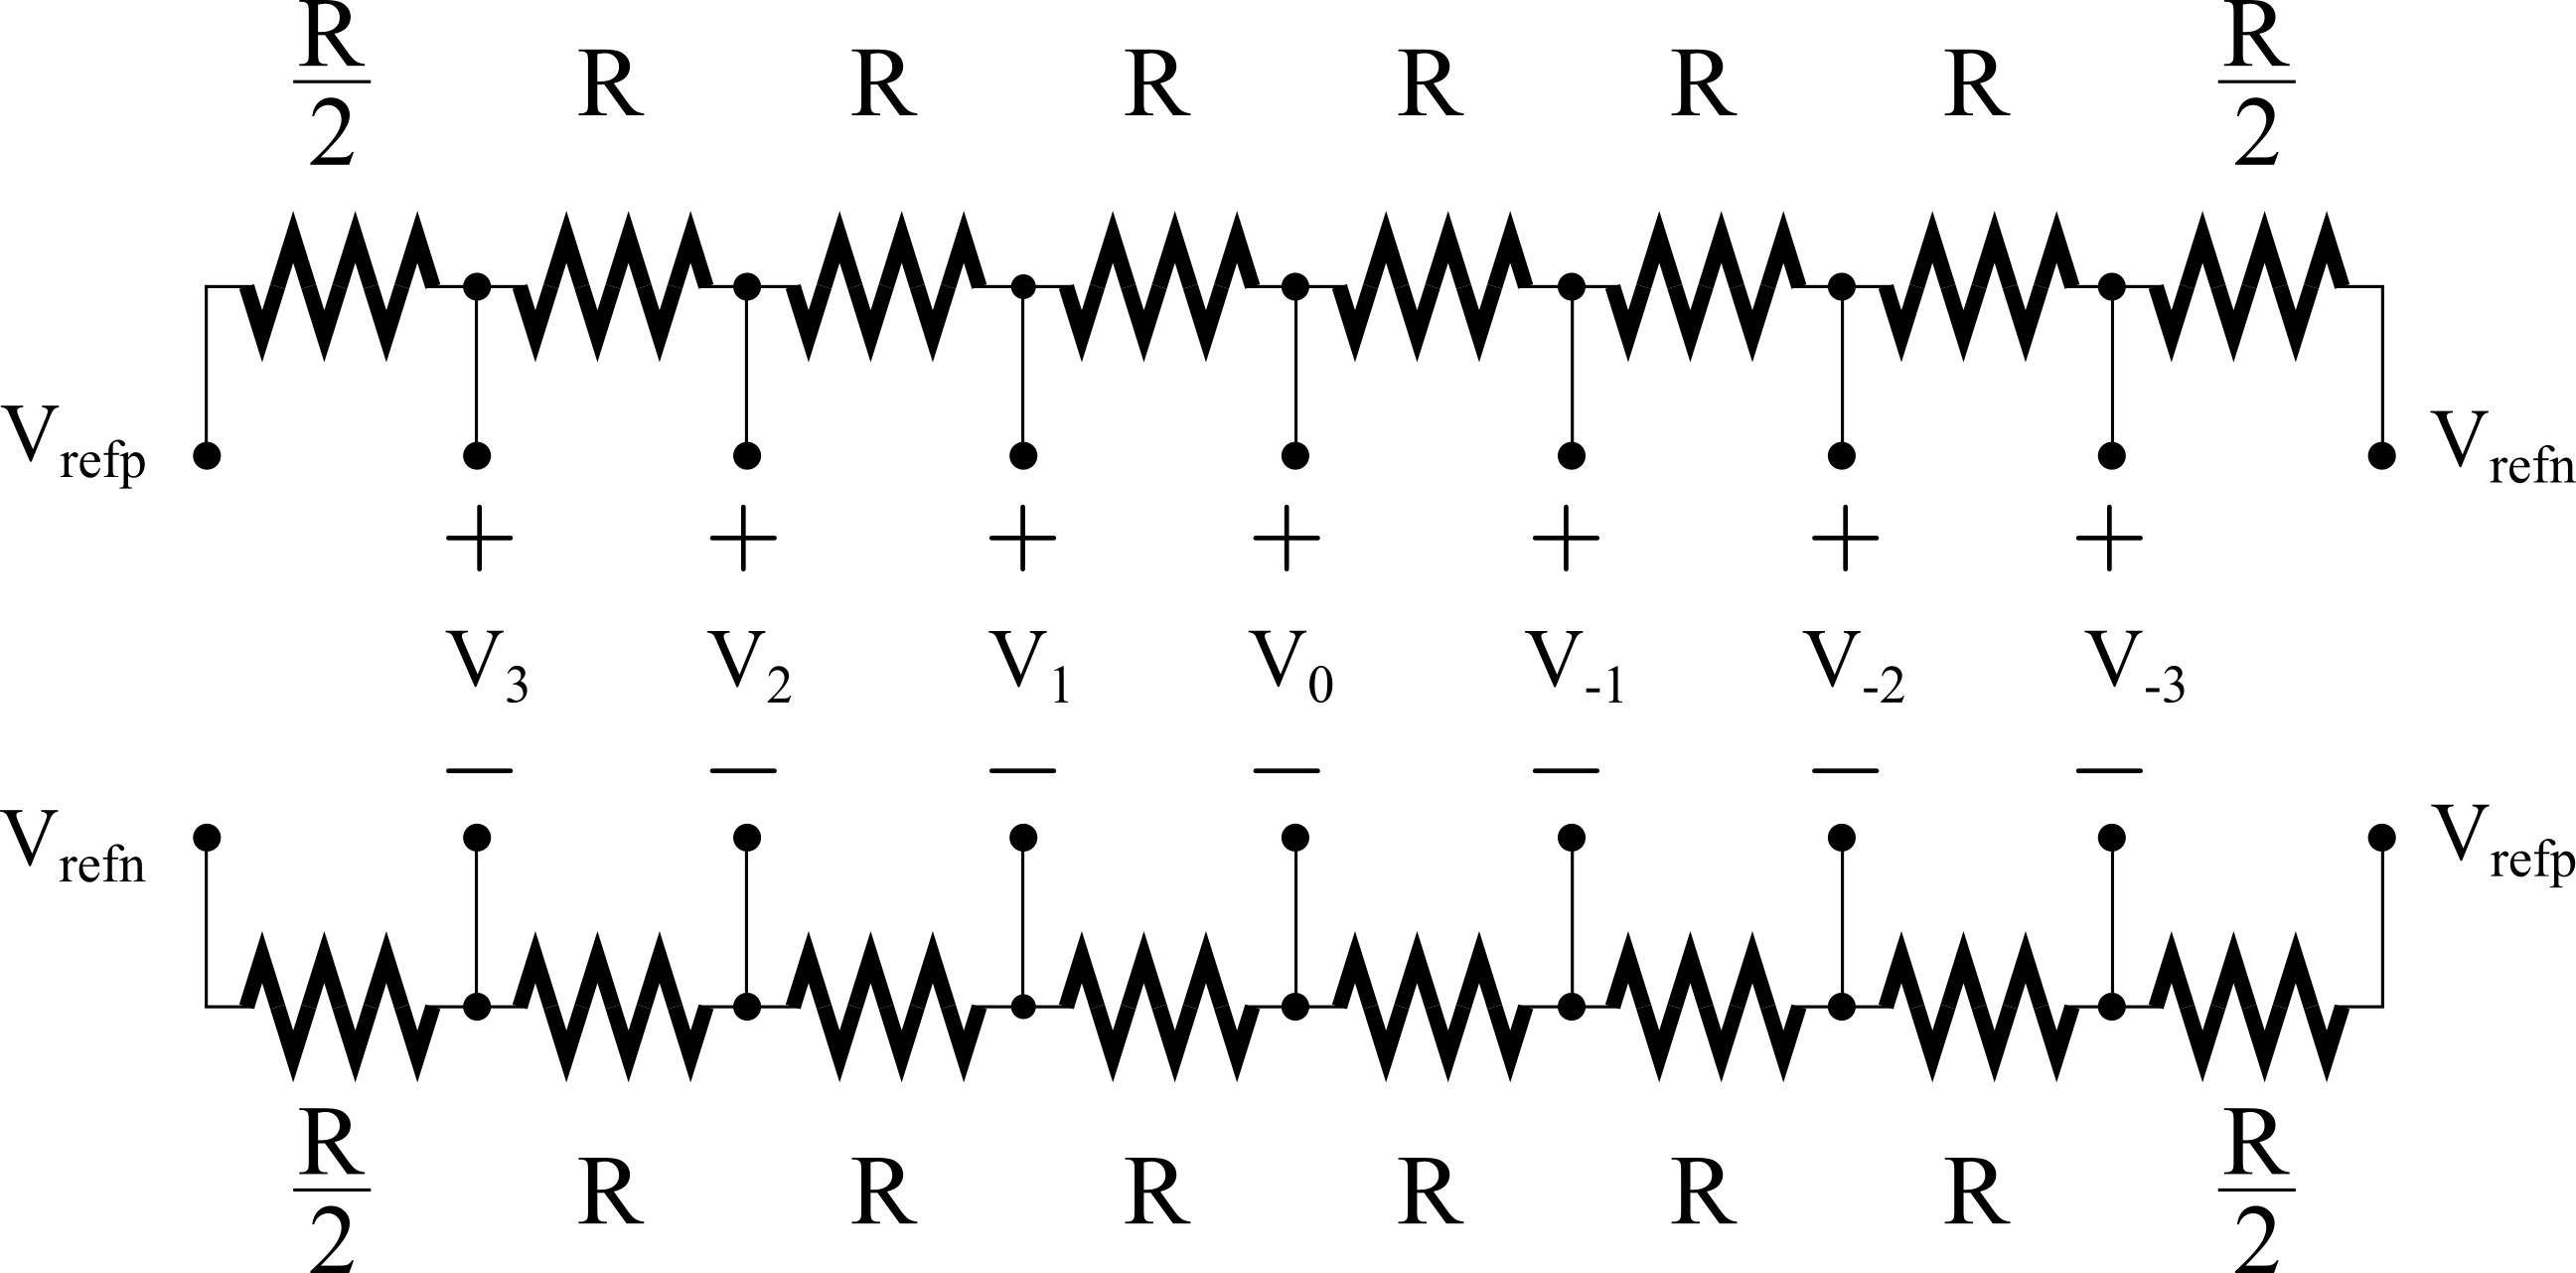
\includegraphics[width=0.85\columnwidth]{Chap05/Figures/resistive_ladder.png}
\caption{Resistive Ladder generating differential threshold voltages for comparators}
\label{fig:res_lad}
\end{figure}
%
But as it is known, the noise in the resistor is proportional to it's value, i.e. $V_{noise}^2=4kTR$, increase in the resistance in order to save the power would end up in noisy thresholds which will then corrupt the comparator decision causing degradation in the performance.

A switched-capacitor arrangement can be employed as an option to the resistive-ladder as shown in Fig. \ref{fig:switched_cap} which saves the static power consumption.
%
\begin{figure}[h!]
\centering
\subfigure[]{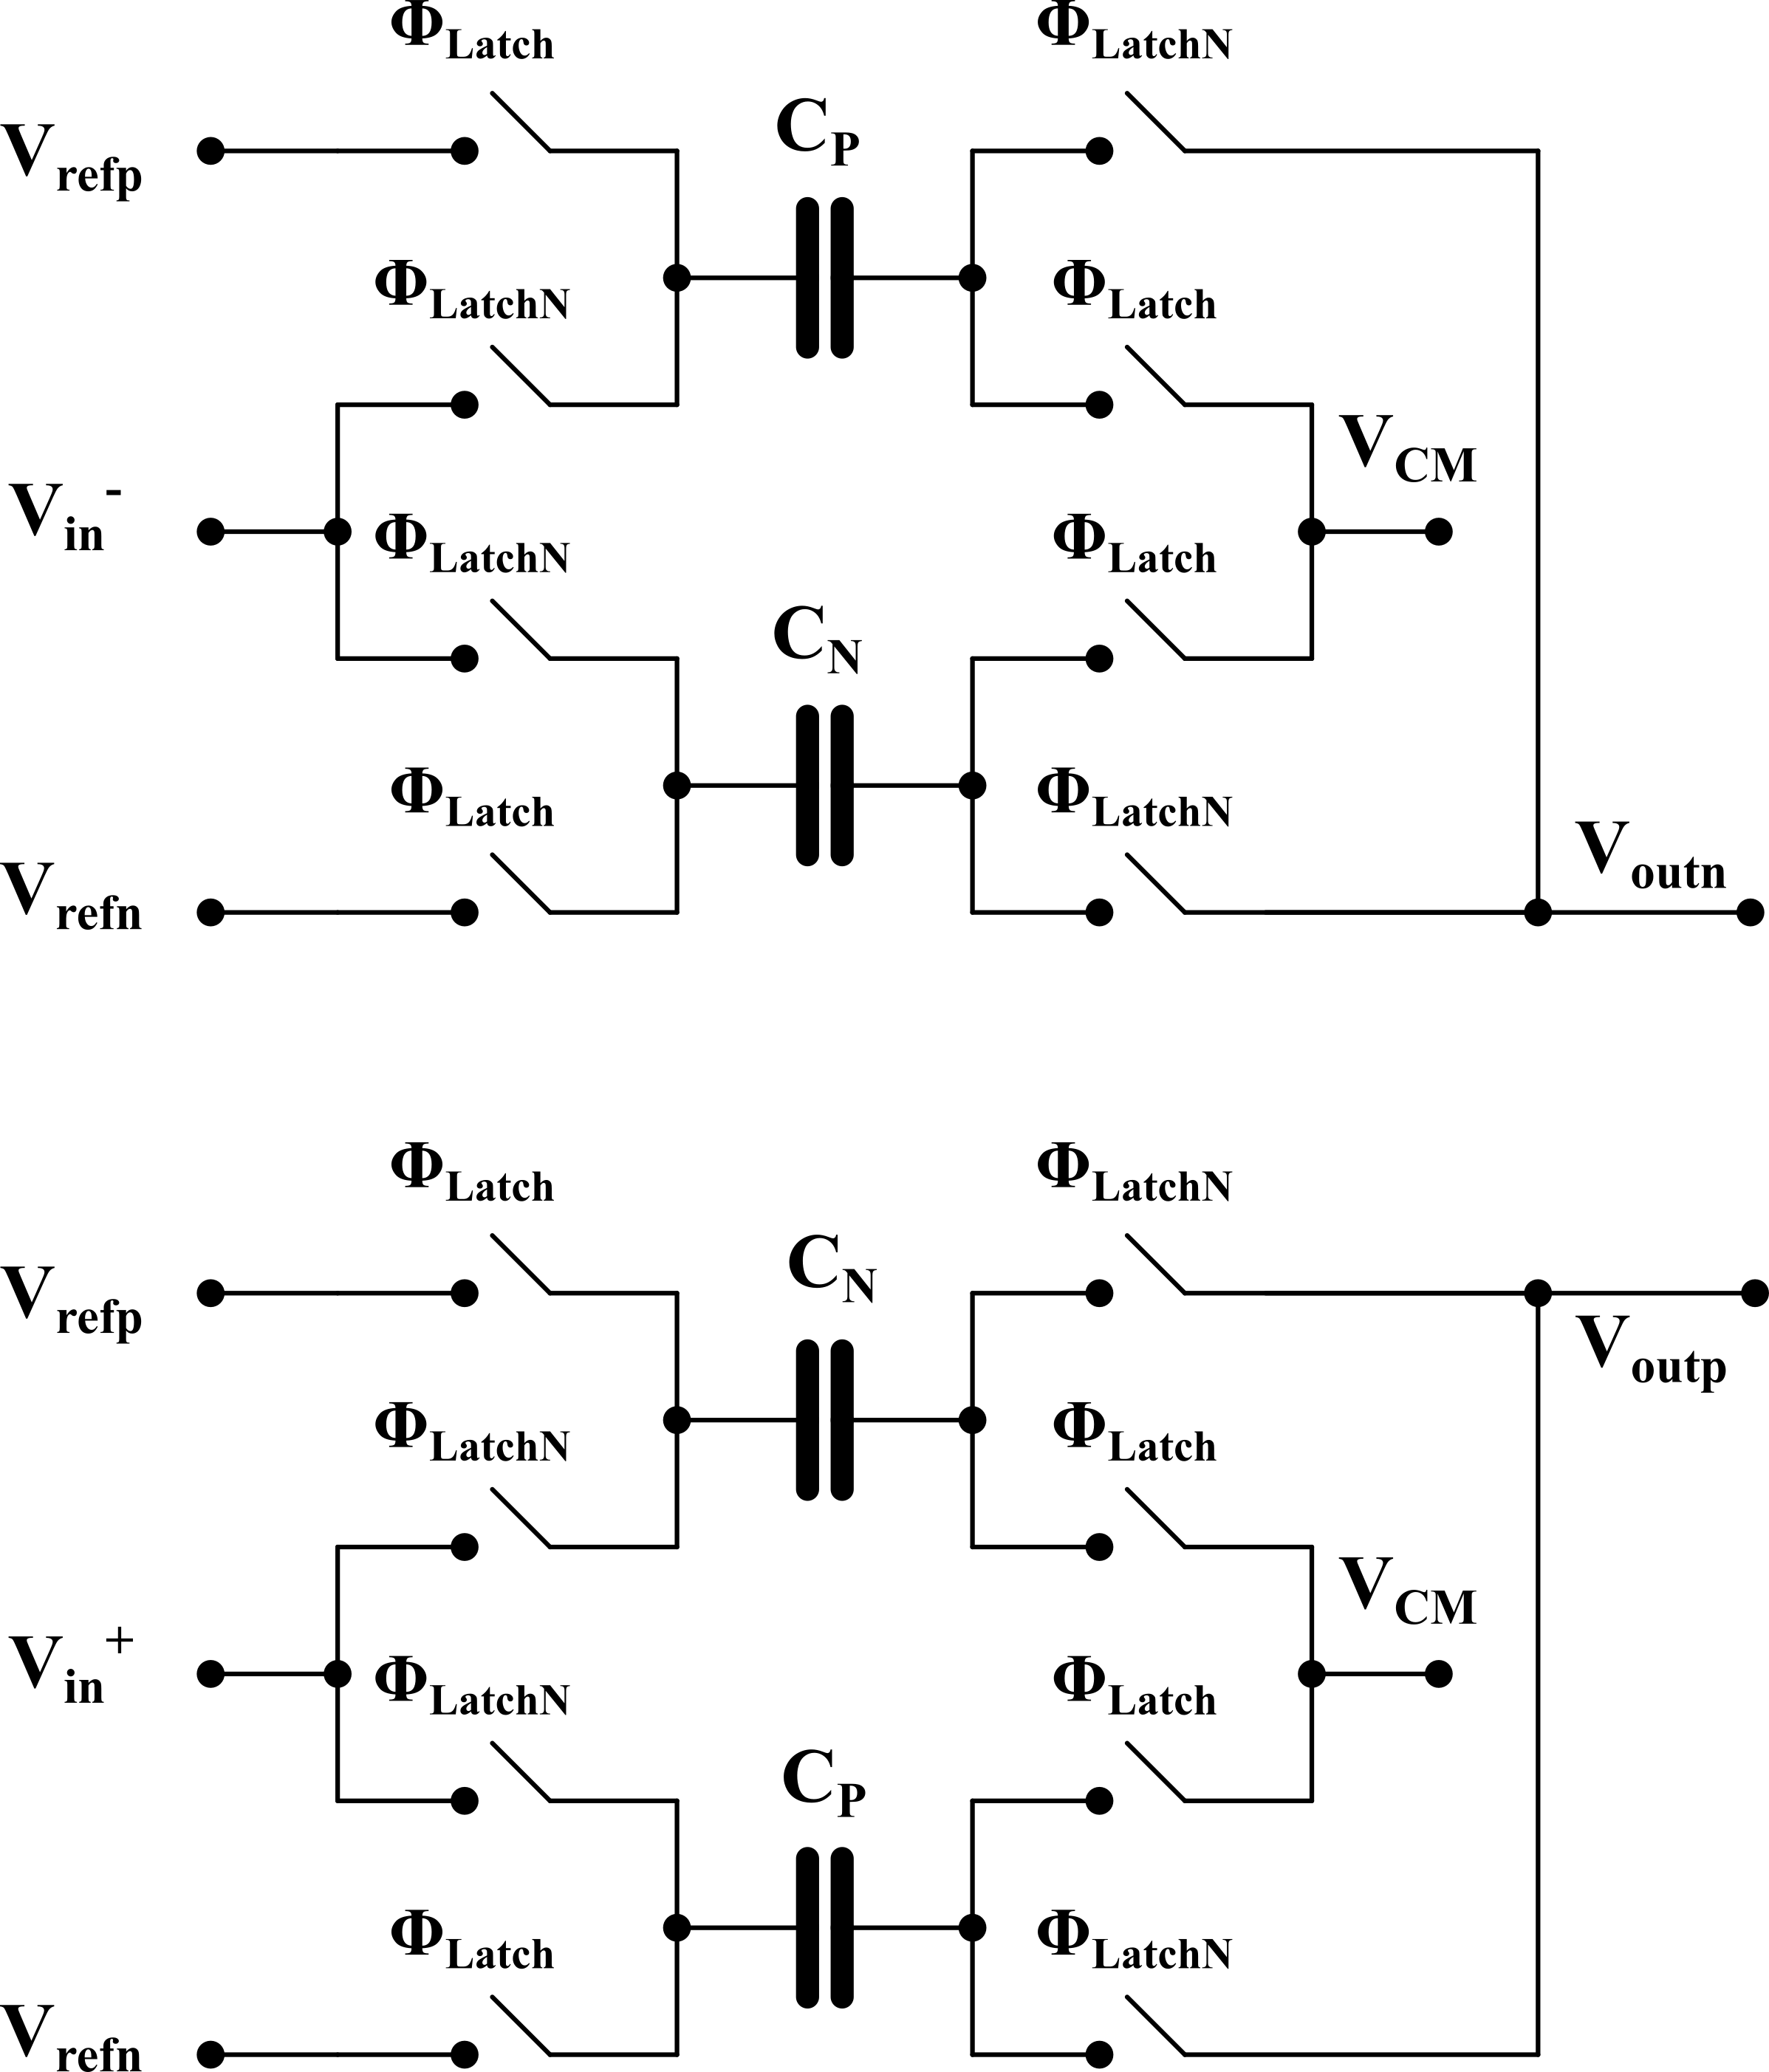
\includegraphics[scale=.32]{Chap05/Figures/switched_cap_thr.png}}\\
\qquad
\subfigure[]{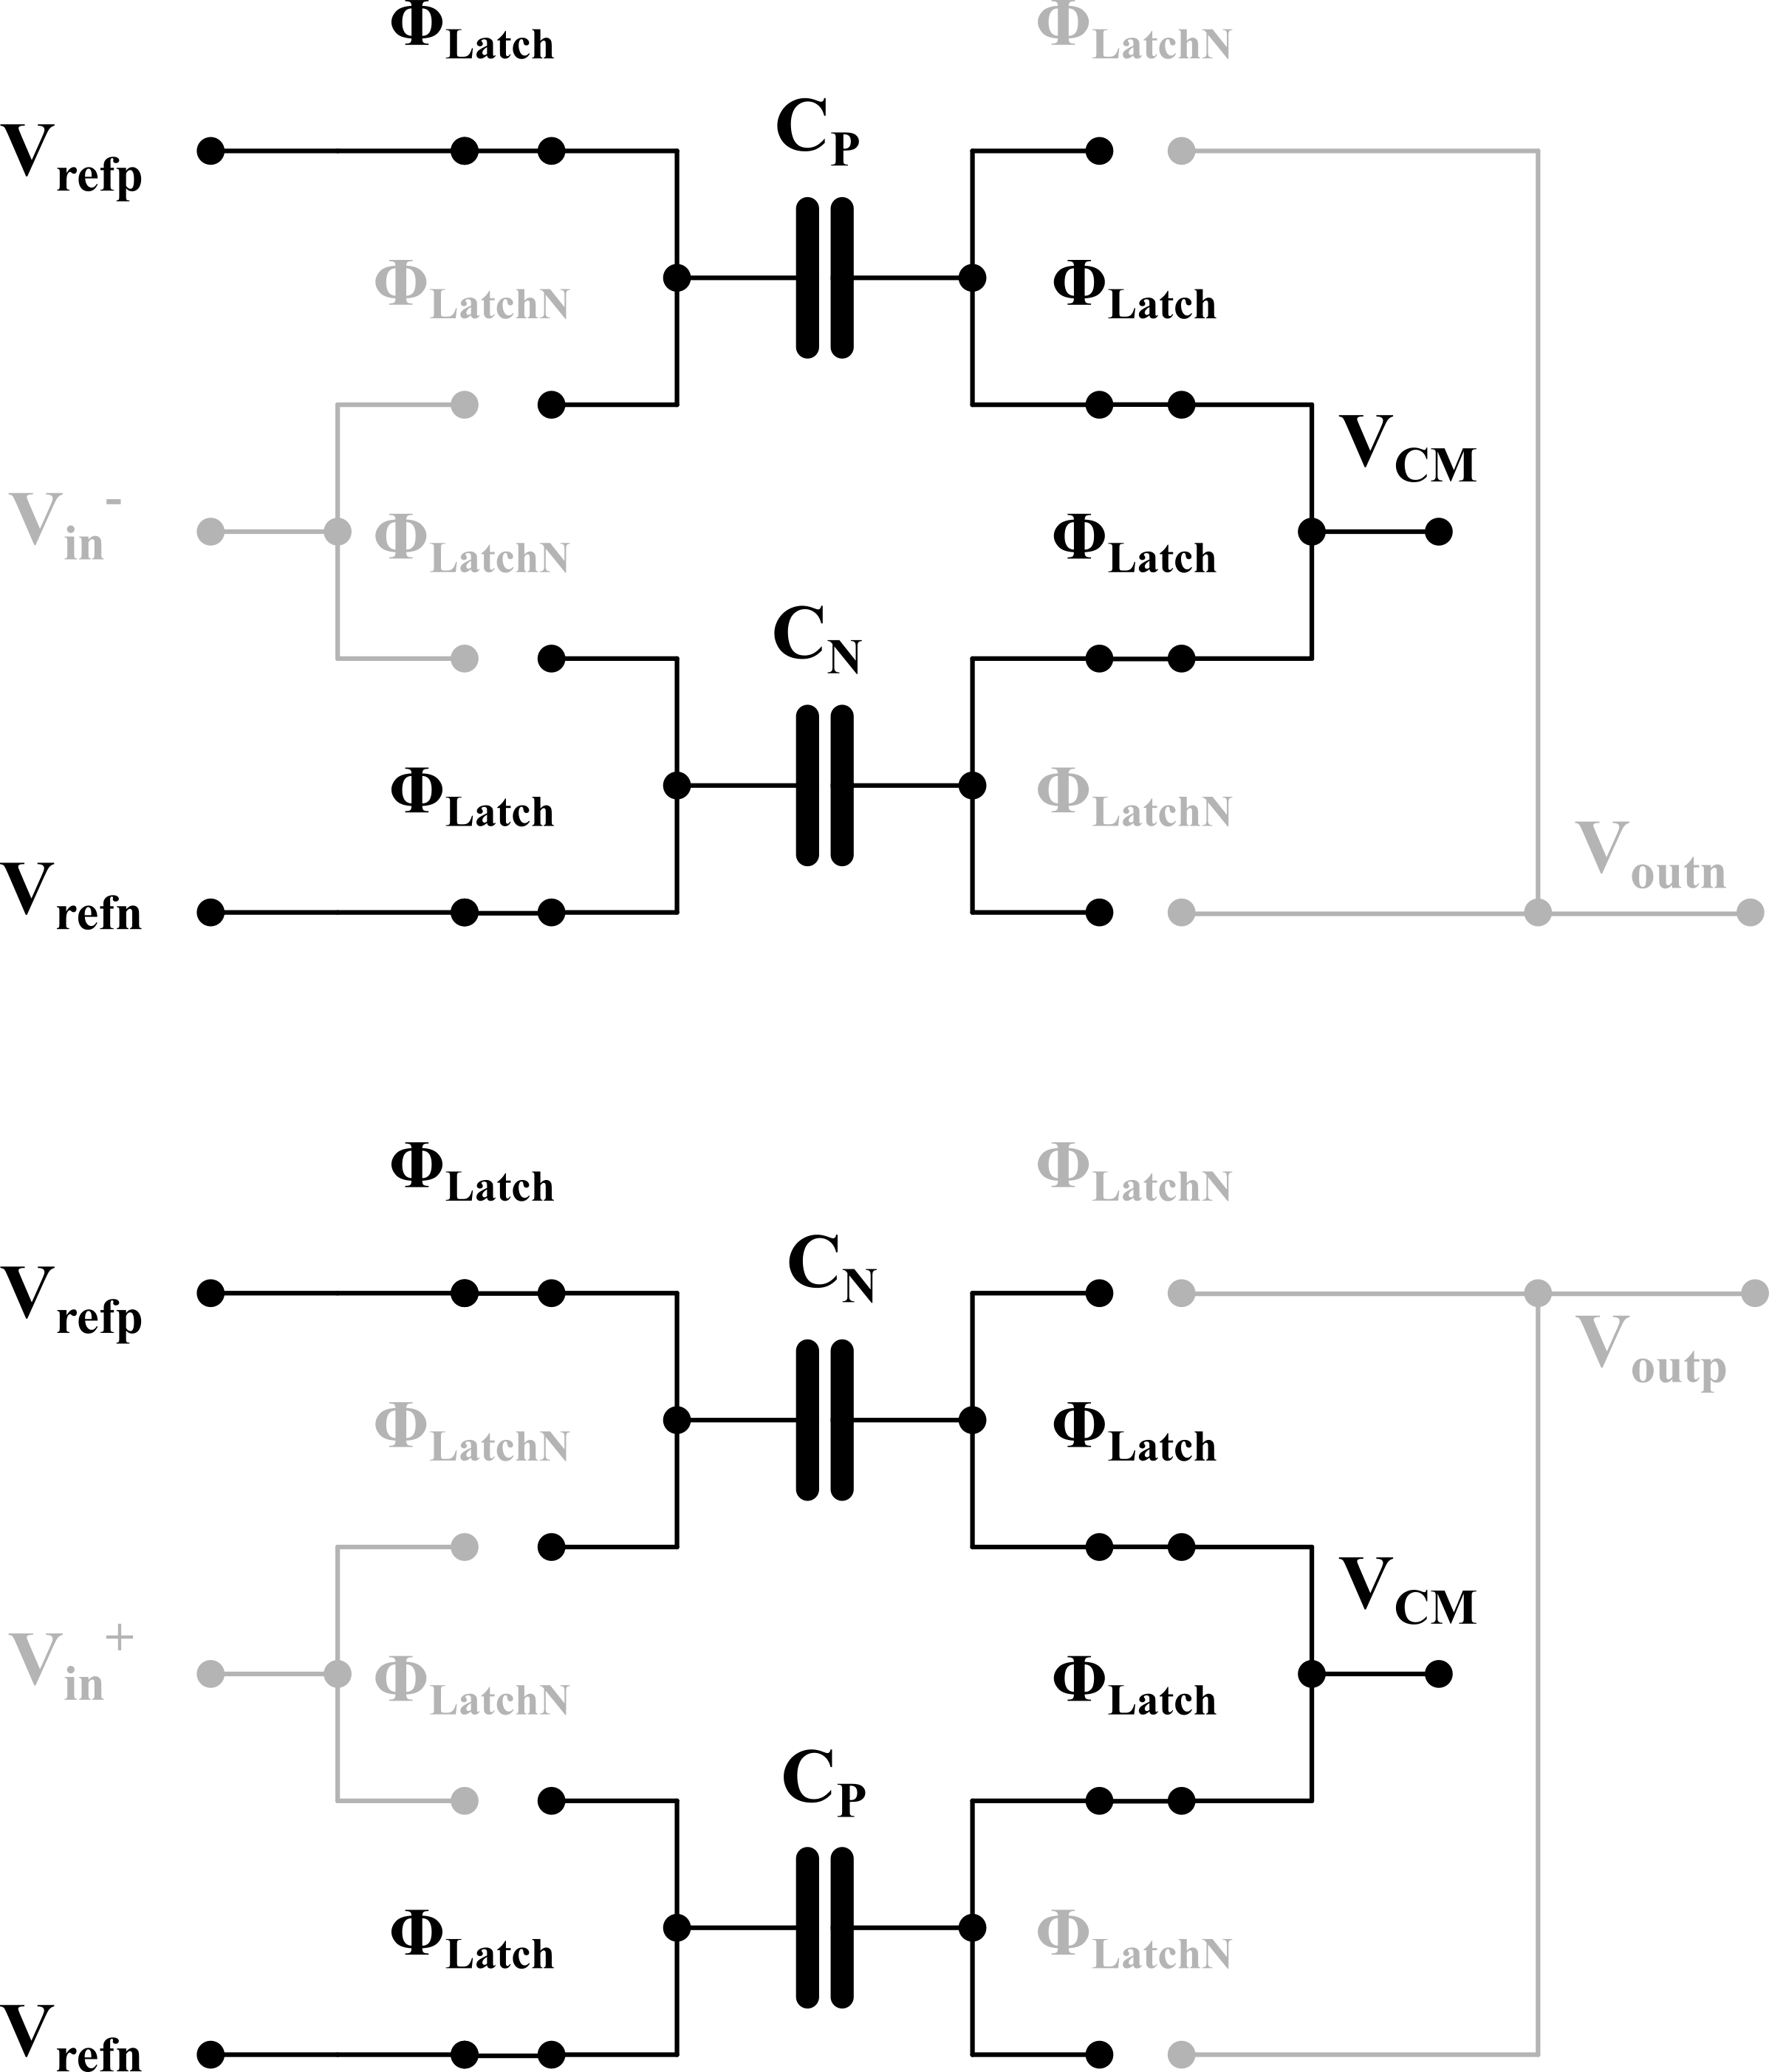
\includegraphics[scale=.32]{Chap05/Figures/switched_cap_thr_latch.png}}
\qquad
\subfigure[]{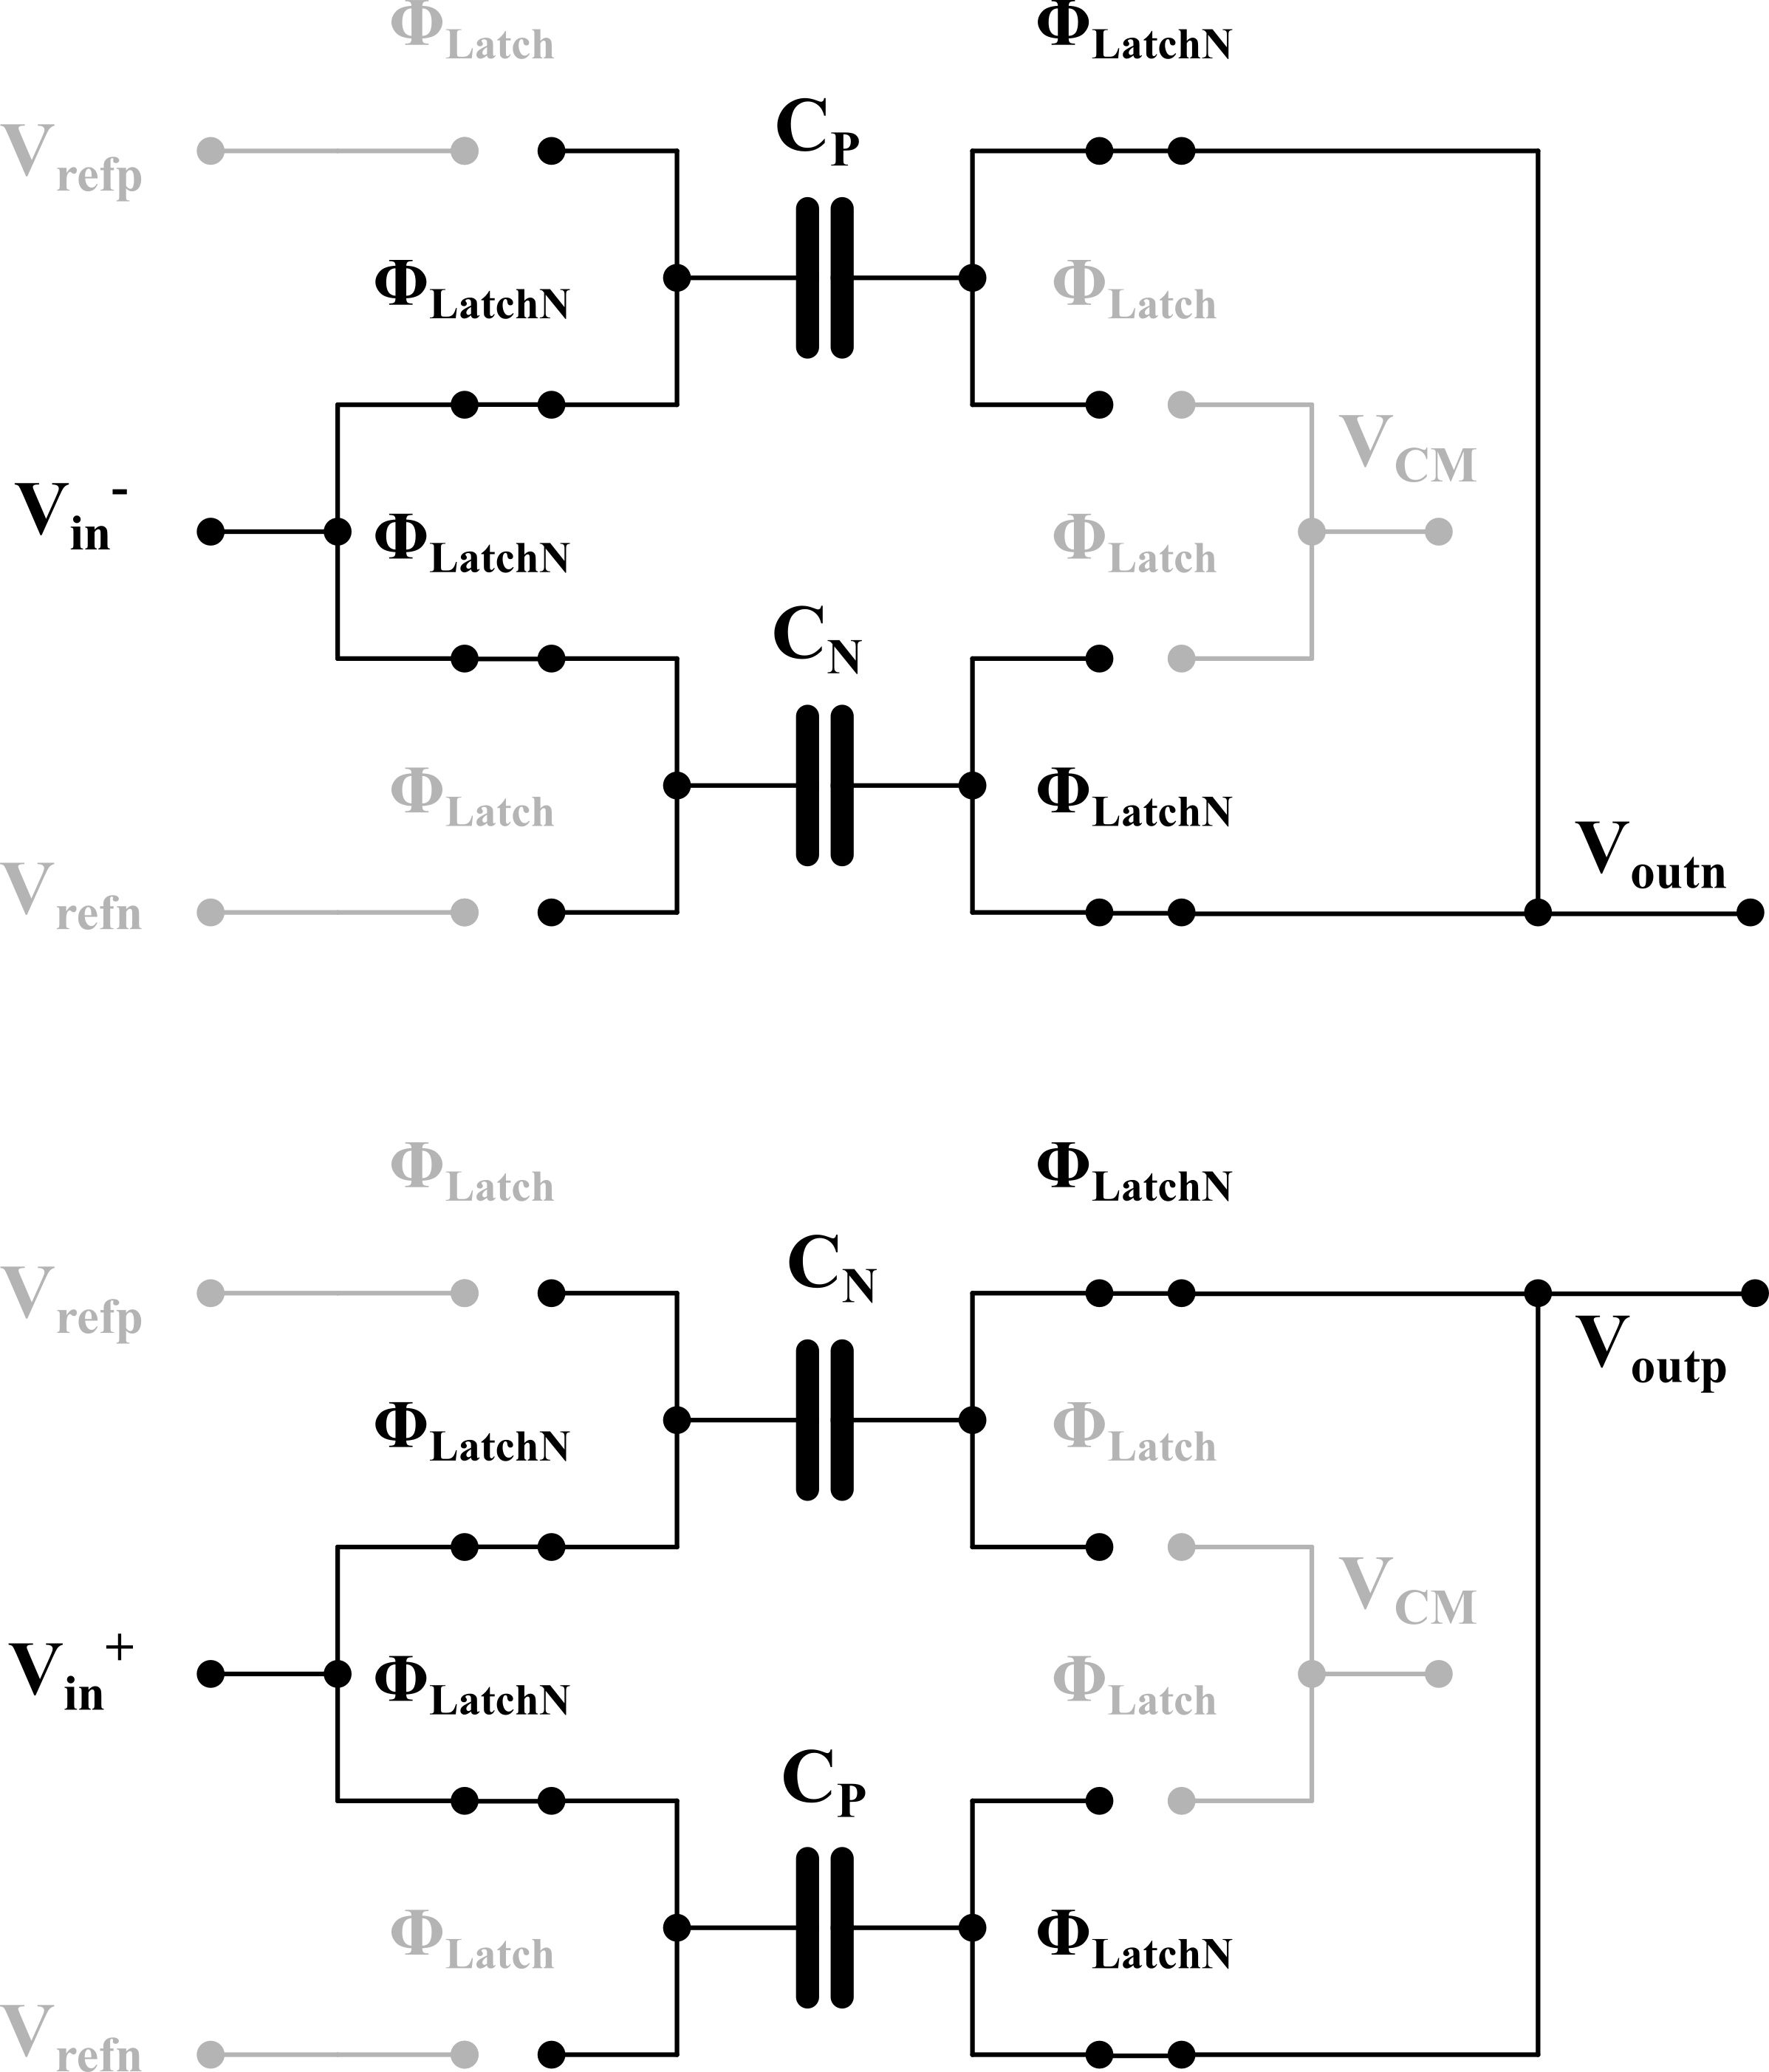
\includegraphics[scale=.32]{Chap05/Figures/switched_cap_thr_latchN.png}}
\caption{(a)Switched capacitor arrangement to generate threshold and taking difference with input sample (b)Threshold generator in a phase sampling reference voltage (c)Threshold generator in a phase sampling signal voltage}
\label{fig:switched_cap}
\end{figure}
%
In the Fig. \ref{fig:switched_cap}(a), the configuration of threshold generator is shown where the reference voltage is sampled on the capacitors with respect to the common mode voltage. Therefore, the charge stored on capacitors $C_{P_{U}}$, $C_{N_{U}}$, $C_{P_{L}}$ and $C_{N_{L}}$ are, ($C_{P_{U}}$=$C_{P_{L}}$=$C_P$, $C_{N_{U}}$=$C_{N_{L}}$=$C_N$)
%
\begin{equation}
    \begin{split}
        Q_{CP_{U}} &= C_{P_{U}}V_{refp} =C_PV_{refp}\\
        Q_{CN_{U}} &= C_{N_{U}}V_{refn} =C_NV_{refn}\\
        Q_{CP_{L}} &= C_{P_{L}}V_{refn} =C_PV_{refn}\\
        Q_{CN_{L}} &= C_{N_{L}}V_{refp} =C_NV_{refp}
    \end{split}
\end{equation}
%
In the next phase where the input signal is sampled, the capacitors $C_{P_{U}}$ and $C_{N_{U}}$ are in parallel which makes it $C_U=C_{P_{U}}+C_{N_{U}}$. Similarly, $C_{P_{L}}$ and $C_{N_{L}}$ parallel combination exhibit the total equivalent capacitance of $C_L=C_{P_{L}}+C_{N_{L}}$. Then the charge and voltage across the capacitors $C_U$ and $C_L$ can be given by,
%
\begin{equation}
    \begin{split}
        Q_{CU} &= Q_{CP_{U}}+Q_{CN_{U}}\\
        (C_P+C_N)V_{CU} &= C_PV_{refp}+C_NV_{refn}
    \end{split}
\end{equation}
%
%
\begin{equation}
        V_{CU}=\frac{C_PV_{refp}+C_NV_{refn}}{C_P+C_N}
\end{equation}
%
similarly,
%
\begin{equation}
        V_{CL}=\frac{C_PV_{refn}+C_NV_{refp}}{C_P+C_N}
\end{equation}
%
Then the voltage difference of $V_{outp}$ and $V_{outn}$ can be expressed as,
%
\begin{equation}
    \begin{split}
        V_{out} &= V_{outp}-V_{outn}\\
                &= (V_{in}^--V_{CU})-(V_{in}^+-V_{CL})\\
                &= \left(V_{in}^--\frac{C_PV_{refp}+C_NV_{refn}}{C_P+C_N}\right)-\left(V_{in}^+-\frac{C_PV_{refn}+C_NV_{refp}}{C_P+C_N}\right)\\
                &= \left(V_{in}^+-V_{in}^-\right)-\frac{C_P-C_N}{C_P+C_N}\left(V_{refp}-V_{refn}\right)\\
                &= V_{in}-V_{thr}
    \end{split}
\end{equation}
%
where the threshold voltage generated by the switched capacitor is,
%
\begin{equation}\label{THR_GEN}
    V_{thr} = \frac{C_P-C_N}{C_P+C_N}\left(V_{refp}-V_{refn}\right)
\end{equation}
%
and, $V_{ref}= V_{refp} - V_{refn}$. 

For multi-bit quantizer, the different values of $C_P$ and $C_N$ generates the different values of the threshold voltages while the total capacitance $C_P+C_N$ is equal. The following table shows the different values of the threshold voltages created by the switched-capacitor block shown in Fig. \ref{fig:switched_cap}, for 3-bit quantizer.
\begin{table}[h!]
\centering
\begin{tabular}{c|c|c}
\Xhline{4\arrayrulewidth}
\textbf{C\textsubscript{P}}      & \textbf{C\textsubscript{N}}      & \textbf{V\textsubscript{thr}} (Volts)     \\ \hline
350 fF                             & 50  fF                             & (3/4)V\textsubscript{ref} \\ \hline
300 fF                             & 100 fF                             & (2/4)V\textsubscript{ref} \\ \hline
250 fF                             & 150 fF                             & (1/4)V\textsubscript{ref} \\ \hline
200 fF                             & 200 fF                             & (0/4)V\textsubscript{ref} \\ \hline
150 fF                             & 250 fF                             & -(1/4)V\textsubscript{ref} \\ \hline
100 fF                             & 300 fF                             & -(2/4)V\textsubscript{ref} \\ \hline
50  fF                             & 350 fF                             & -(3/4)V\textsubscript{ref} \\ \Xhline{4\arrayrulewidth}
\end{tabular}
\caption{The threshold voltages generated for 3-bit quantizer}
\label{tab:vthr}
\end{table}

However, since the signal swing at the output of second integrator is reduced 4 times, which is the input to the quantizer, the signal do not cover full range of the quantizer but just $1/4^{th}$ part of the full-scale. This will result in the decreased SQNR as a consequence. In order for input signal to quantizer to cover the full-scale, now, solution is to scale the quantizer thresholds down by equal amount as the signal, i.e. by a factor of 4. The ratios of the capacitors in the threshold generator has to be modified as follows considering the unit capacitance of $C_{unit}=12.5~fF$ which still accounts the total capacitance $C_P~+~C_N~=~400~fF$ 
%
\begin{table}[h!]
\centering
\begin{tabular}{l|l|r}
\Xhline{4\arrayrulewidth}
\multicolumn{1}{c|}{\textbf{C\textsubscript{P}}}        & \multicolumn{1}{c|}{\textbf{C\textsubscript{N}}}     & \multicolumn{1}{c}{\textbf{V\textsubscript{thr}}}       \\ \hline
19C\textsubscript{unit} = 237.5 fF & 13C\textsubscript{unit} = 162.5 fF & (3/16)V\textsubscript{ref}  \\ \hline
18C\textsubscript{unit} = 225 fF      & 14C\textsubscript{unit} = 175 fF   & (2/16)V\textsubscript{ref}  \\ \hline
17C\textsubscript{unit} = 212.5 fF    & 15C\textsubscript{unit} = 187.5 fF & (1/16)V\textsubscript{ref}  \\ \hline
16C\textsubscript{unit} = 200 fF      & 16C\textsubscript{unit} = 200 fF   & (0/16)V\textsubscript{ref}  \\ \hline
15C\textsubscript{unit} = 187.5 fF    & 17C\textsubscript{unit} = 212.5 fF & -(1/16)V\textsubscript{ref} \\ \hline
14C\textsubscript{unit} = 175 fF      & 18C\textsubscript{unit} = 225 fF   & -(2/16)V\textsubscript{ref} \\ \hline
13C\textsubscript{unit} = 162.5 fF    & 19C\textsubscript{unit} = 237.5 fF & -(3/16)V\textsubscript{ref} \\ \Xhline{4\arrayrulewidth}
\end{tabular}
\caption{Modified threshold voltages, generated for 3-bit quantizer accommodating the signal to full scale.}
\label{tab:vthr_mod}
\end{table}
%
\subsection{Comparator}
The architecture of the comparator used in the quantizer is as shown in the Fig. \ref{COMP} which is designed to work with a clock frequency of $80\ MHz$. The driving transistors pair $M_{0}$ and $M_{1}$, constitutes a preamplifier. It amplifies the signal prior to the comparison and transmits it to the back-to-back connected NOT gate.
\begin{figure}[h!]
\centering
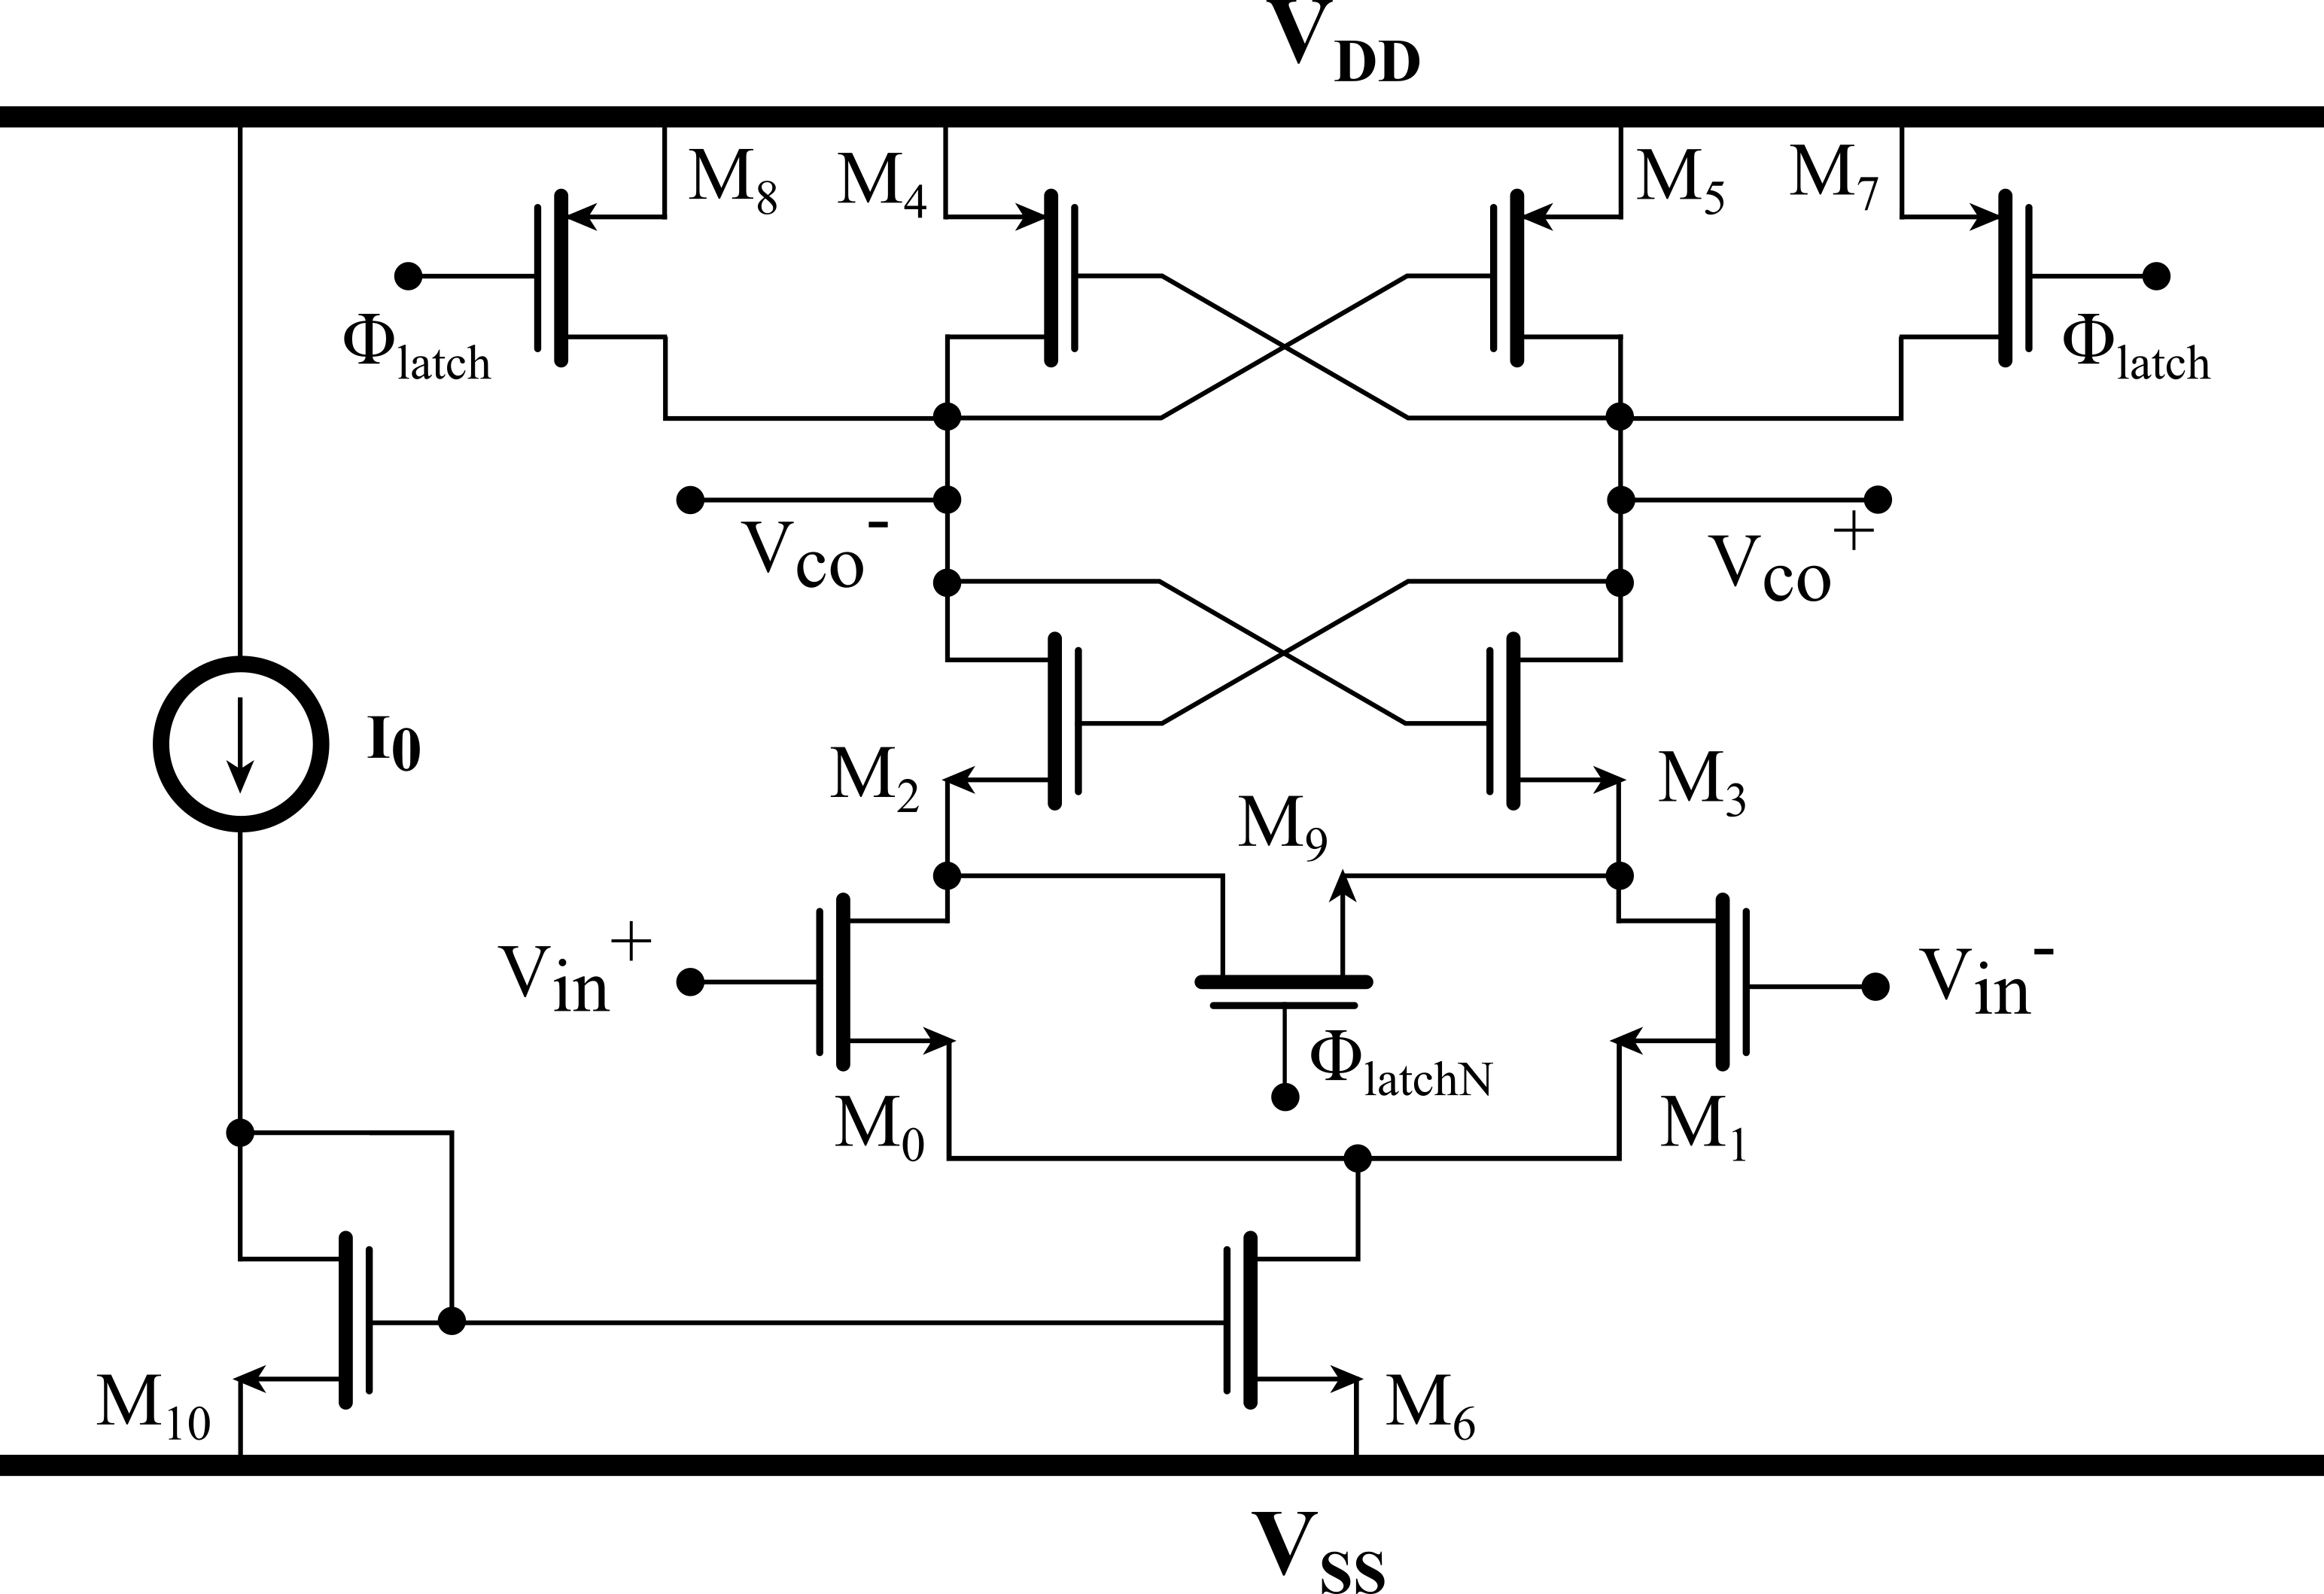
\includegraphics[width=0.8\columnwidth]{Chap05/Figures/comparator.png}
\caption{Schematic of the Comparator employed in the Quantizer}
\label{COMP}
\end{figure}
 This is a positive feedback circuit which pulls up or down the output node ($V_{CO}^+$ and $V_{CO}^-$) voltage depending on the signal transferred from the preamplifier and takes the decision.
These comparison signals can then be stored in the latch comprised of NAND gates and then are passed through the buffers to make the signals strong enough to drive the given load as shown in the Fig. \ref{LATCH}.
\begin{figure}[h!]
\centering
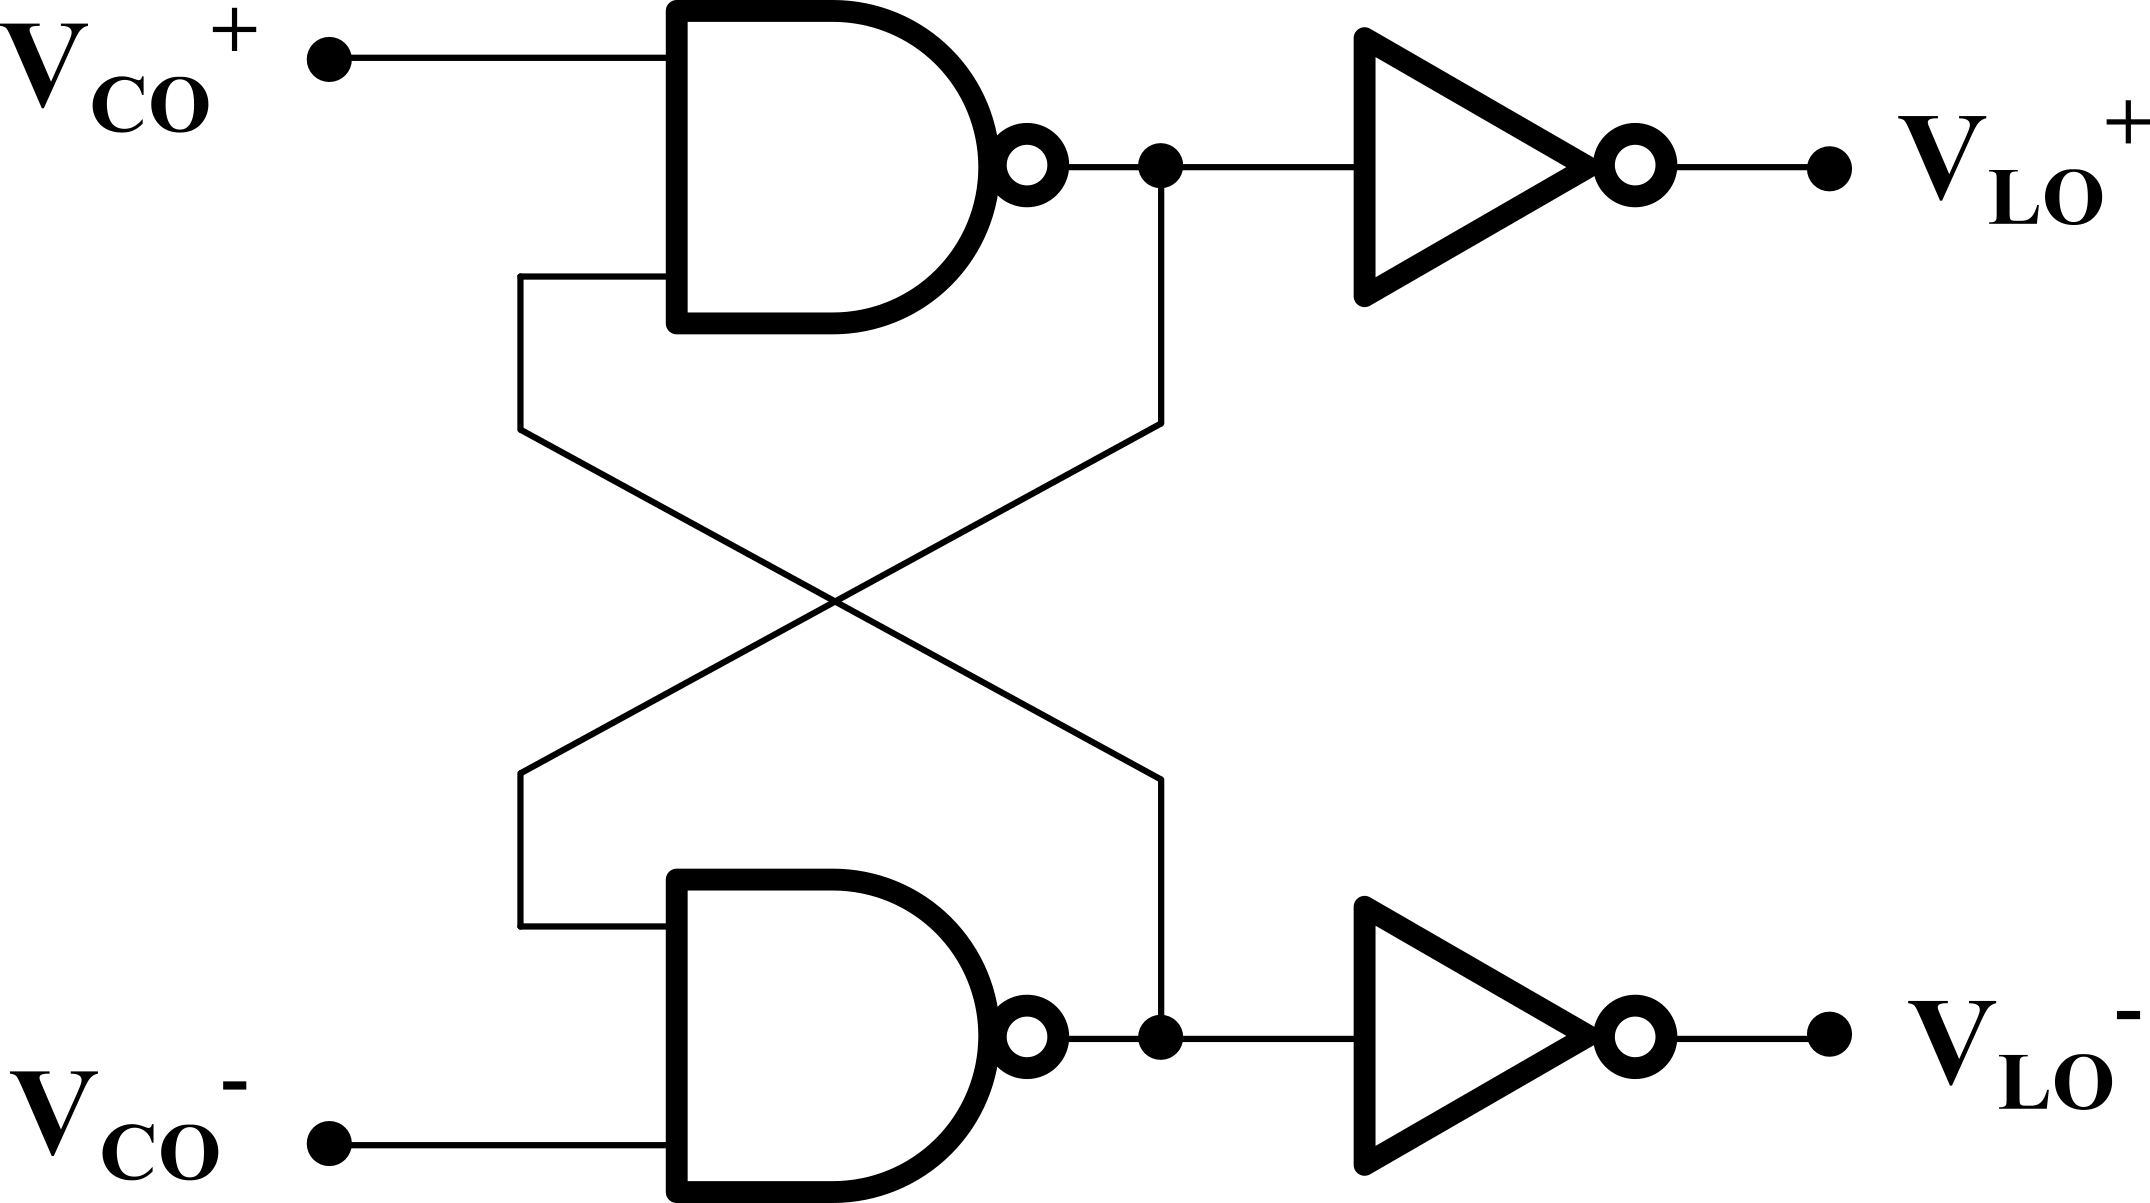
\includegraphics[width=0.5\columnwidth]{Chap05/Figures/latch.png}
\caption{Latch Comprised of NAND gates and digital buffers}
\label{LATCH}
\end{figure}
The capacitive divider is used to generate the threshold, specific for a comparator and it's value depends on the ratio of the capacitors, can be expressed as in the Eq. \ref{THR_GEN}.
\begin{figure}[h!]
\centering
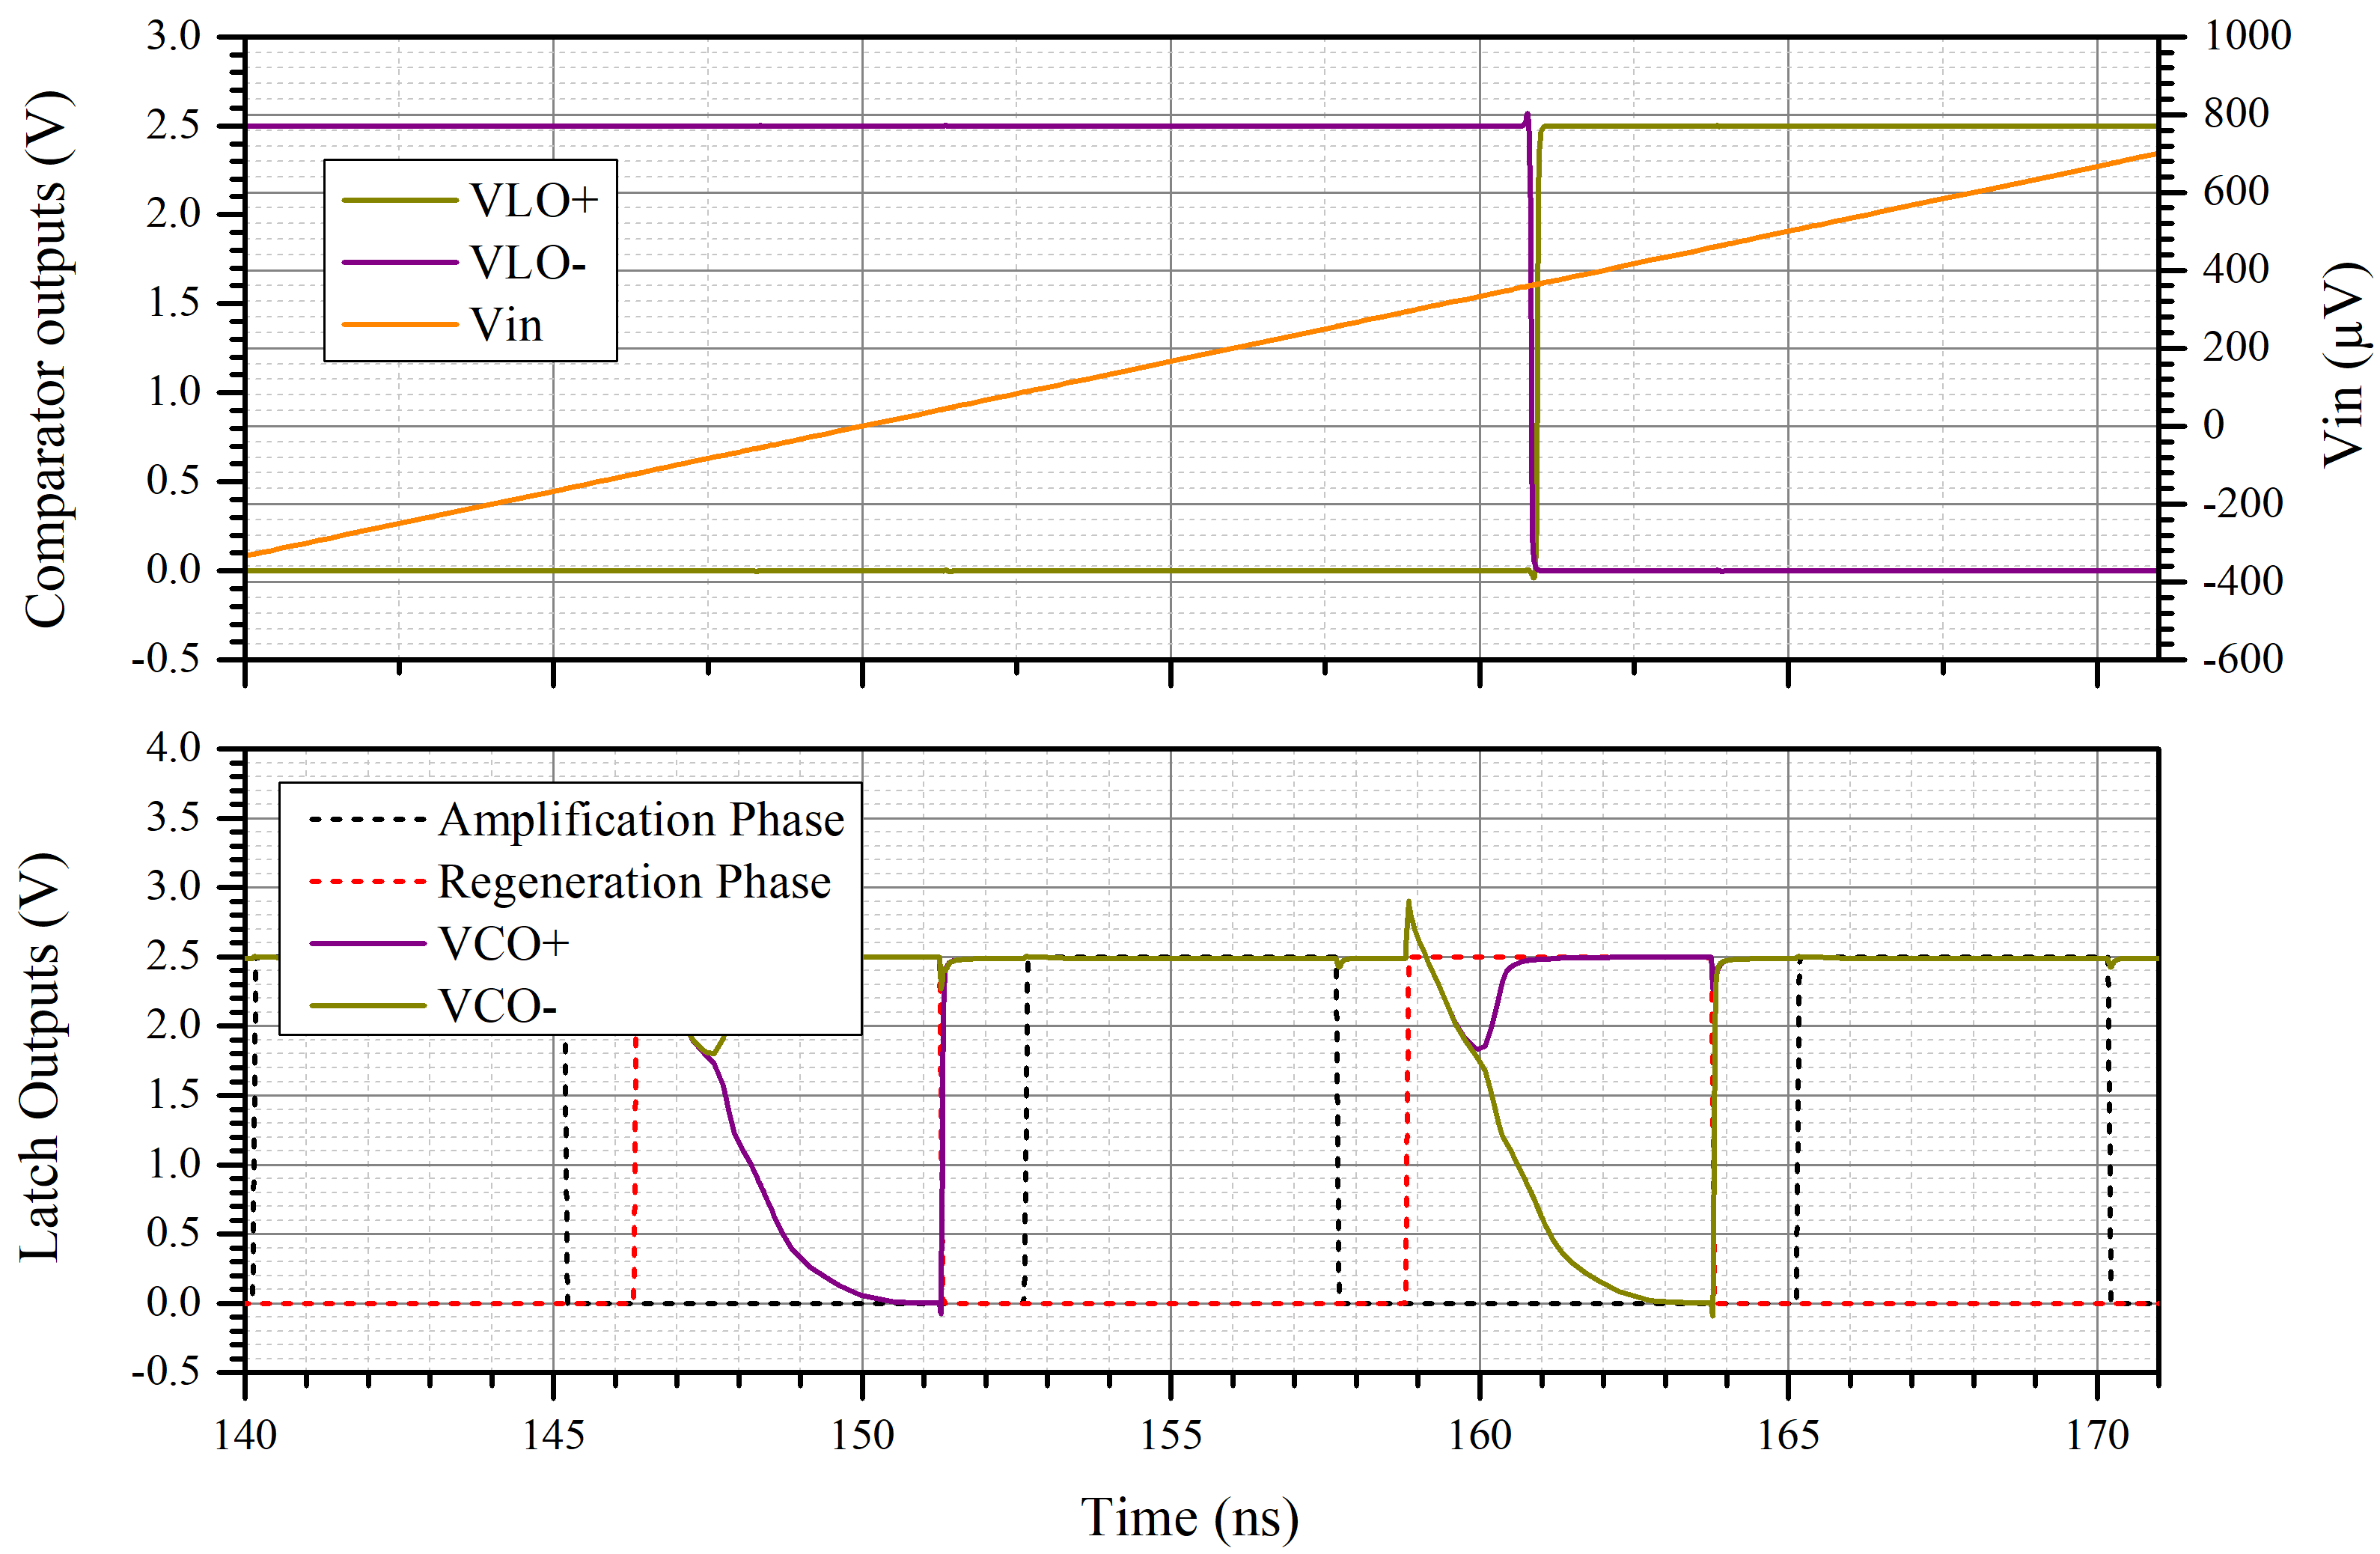
\includegraphics[width=\columnwidth]{Chap05/Figures/comparator_signals.png}
\caption{Signals at the different nodes of the Comparator}
\label{fig:comp_sigs}
\end{figure}
The simulation results of the comparator in Fig. \ref{LATCH} are shown in the Fig. \ref{fig:comp_sigs}. In the simulation set-up the negative terminal of the comparator ($V_{in}^-$) is kept constant at the common-mode voltage ($V_{CM}=1.25~V$) while the positive terminal ($V_{in}^+$) is linearly varied from ($V_{CM}-10~mV$) to ($V_{CM}+10~mV$), while the comparator is clocked at the frequency of 80~MHz. The characteristic in orange in the top plot shows the differential input voltage ($V_{in}^+-V_{in}^-$) in the time frame from $140~ns$ to $171~ns$ which covers two amplification phases and two regeneration phases. In the first amplification phase, from time $140~ns$ to $145~ns$, the differential input voltage is around $-300~\mu V$. Therefore in the regeneration from $146~ns$ to $151~ns$, higher potential on the negative input causes to draw the more current through transistor $M_1$ than that through $M_0$. The rate at which the positive output node ($V_{CO}^+$) is discharging is higher than that the negative node ($V_{CO}-$) discharge rate. In turn, the node $V_{CO}+$ reaches the potential of $V_{DD}-V_{thp}$ first, which is connected to the gate of the transistor $M_4$ turning it $on$ thereby connecting the $V_{DD}$ to the negative output $V_{CO}^-$. This output is connected to the gate of NMOS transistor $M_3$ causing it to turn $on$ and the gate of PMOS transistor $M_5$ turning it $off$ which discharges the node to ground very fast. These outputs from comparator are then provided to the SR latch which stores the decision with outputs $V_{LO}^+$ and $V_{LO}^+$ as shown in the top plot of Fig. \ref{fig:comp_sigs}.

In the next amplification phase, the differential input is positive and is around $200~\mu V$. Therefore exactly counter-operation in the comparator will take place in regeneration phase pulling the $V_{CO}^-$ to ground and pushing $V_{CO}^+$ node to $V_{DD}$ as shown in the bottom plot of the Fig. \ref{fig:comp_sigs}.
\begin{figure}[h]
\centering
\includegraphics[width=0.75\columnwidth]{Chap05/Figures/comp_thr.png}
\caption{A complete structure of Comparator}
\label{COMP_THR}
\end{figure}

A complete structure of the comparator is shown in Fig. \ref{COMP_THR} which consists of a switched-capacitor threshold generator and the next block is pre-amplifier and the back-to-back connected NOT for amplification and regeneration. This is the one slice of the whole quantizer. In case of 3-bit quantizer, there will be such a 7 slices with different values of $C_P$ and $C_N$ generating 7 different thresholds as shown in Tab. \ref{tab:vthr_mod}.
\section{DAC Architecture}
\begin{figure}[h]
\centering
\includegraphics[width=\columnwidth]{Chap05/Figures/dac.png}
\caption{A 3-bit Thermometric Capacitive DAC at the input of First integrator}
\label{DAC}
\end{figure}
Since, the quantizer implemented in the IADC is of the resolution of 3-bit, the architecture of the DAC employed needs to be of the same resolution. Therefore the capacitive DAC with thermometric inputs is realized as shown in the Fig. \ref{DAC}. In the phase $\Phi_{input}$, the input signal is sampled on the array of unit capacitors comprising the sampling capacitor while in the phase $\Phi_{DACn}$, the feedback signal from the quantizer is sampled and thus a difference between input signal and the digital equivalent of the input signal i.e. residue is integrated.
Here, $\Phi_{DACn} = \Phi_{DAC}*b_n$ and $\overline{\Phi_{DACn}} = \Phi_{DAC}*\overline{b_n}$ where $b_n$ and $\overline{b_n}$ are the $n^{th}$ thermometric output and it's complement from the quantizer and the $\Phi_{DAC}$ is the phase when feedback DAC signal should be applied. 


\section{Inter-Stage Gain Block}

\begin{figure}[h!]
% \centering
\hspace{1in}
\includegraphics[width=0.7\columnwidth]{Chap05/Figures/ISG.png}
\caption{Inter-Stage Gain Block Diagram}
\label{fig:ISG}
\end{figure}

The circuit diagram of the Inter-stage Gain block is shown in Fig.~\ref{fig:ISG}. Since the architecture employed is the modified architecture of the Incremental ADC, the output of the second integrator contains not only the residue but the components proportional to the input signal as well as the output of the first integrator.
%
\begin{equation*}
        y[M]=a_1u[M]+a_2w[M]+a_1a_2\frac{M(M-1)}{2}u-a_1a_2V_{ref}\left(v[M-2]+.....+(M-1)v[0]\right)
\end{equation*}
%
Where the integrator coefficients $a_1=1$ and $a_2=1$ and the feed-forward coefficients $b_1=1$ and $b_2=2$. 

Therefore the ISG block has to first extract the residue by subtracting the input signal and the output of the first integrator from the second integrator's output with proper coefficients and then amplify the residue so as to cover the full-scale of the residual ADC (RADC), i.e.
%
\begin{equation}
    e[M]=y[M]-b_1u[M]-b_2w[M]
\end{equation}
%
%
\begin{equation}
    ISG\ output = G e[M] = G y[M]-G b_1u[M]-G b_2w[M]
\end{equation}
%
Then, the coefficients $b_1=1$ and $b_2=2$ are set by the IADC part while the ISG gain $G$ must be set to $2^{N_{SD}-1}$, i.e. 4, so that the amplified residue covers full-scale of RADC. Then the final coefficients of the input signal $u[M]$, output of first integrator $w[M]$ and the output of second integrator $y[M]$ for the extraction and amplification of residue are constructed by the ratio of the sampling capacitor and the feedback capacitors i.e.
%
\begin{equation}\label{eq:isg_caps}
    \begin{split}
        Coeff.\ of\ y[M]&=\frac{C_{integ2}}{C_F}=4\\
        b_1&=\frac{C_{input}}{C_F}=4\\
        b_2&=\frac{C_{integ1}}{C_F}=8
    \end{split}
\end{equation}
%
However, it should be noted that, the second integrator's output is already reduced by factor of 4 in order to satisfy the swing of the op-amp. Therefore the signals $y[M]$, $u[M]$ and $w[M]$ are smaller by factor of 4. Thus, if the residue has to be amplify to the RADC full-scale (1.2V), the additional amplification factor must be incorporated in inter-stage gain $G$, i.e. overall gain factor will be 16 and the swing will be then 1.2V. 

Nevertheless, it has been seen that achieving such a high voltage swing for given low frequency gain of 50~dB and GBW of 200~MHz is quite difficult. Hence, the ISG gain is set to 4 instead, which brings the residue swing down. Then the capacitance ratios are as shown in the Eq.(\ref{eq:isg_caps})

Note that the residue swing is now $1/4^{th}$ of the reference voltage. It means the overall ERADC signal-to-quantization noise ratio will go down by 12~dB.
%
\begin{figure}[h!]
    \centering
    \includegraphics[width=0.6\columnwidth]{Chap05/Figures/ISG_opamp.png}
    \caption{Single ended representation of the Inter-stage Gain Block in the amplification phase}
    \label{fig:ISG_ampl}
\end{figure}
%

After considering the parasitic capacitance at virtual ground and the output node, the configuration of ISG in the integrating phase looks like as shown in Fig. \ref{fig:ISG_ampl}. Then the total load capacitance and the beta factor can be calculated as,
%
\begin{equation}
    C_{L_{ISG}}=\frac{C_{F}(C_{input}+C_{integ1}+C_{integ2}+C_i)}{C_{F}+C_{input}+C_{integ1}+C_{integ2}+C_i}+C_o
\end{equation}
%
%
\begin{equation}
    \beta_{ISG} = \frac{C_{F}}{C_{F}+C_{input}+C_{integ1}+C_{integ2}+C_i}
\end{equation}
%
The values of the capacitances are $C_{input}=C_{integ2}=400 fF$, $C_{integ1}=800 fF$ while $C_{F}=100 fF$. The parasitics considered prior to the design $C_i=100f$
and $C_o=100f$, which results in the total load capacitance of around $200 fF$ and the feedback factor $\beta = \frac{1}{18}$. However, the op-amp requirements are quite similar to that in the first integrator. Therefore, the similar architecture is employed for the amplifier also in the ISG for the specifications of low-frequency loop gain = 60~dB, and the GBW = 200~MHz for given load and the feedback factor.


\section{Supporting Blocks}
The two integrators, multi-bit quantizer, feedback DAC and the inter-stage gain block are the core blocks of the ERADC architecture where the functionality of the structure can be verified. However, few more blocks are needed to incorporate along with core blocks such as biasing block which is used to bias the op-amps in the integrators and the inter-stage gain block as well as the comparators in the quantizer, the timing block to generate various phases such as $\Phi_1$, $\Phi_2$ etc and some spacial signals such as End-of-Conversion ($\Phi_{EOC}$), reset integrators ($\Phi_{RST}$), the Dynamic Element Matching (DEM) to improve the linearity of the feedback DAC etc.

\subsection{Biasing}
There are op-amps in the two integrators and the ISG block and the comparators in the quantizer which need the biasing current of $10~\mu A$. Therefore a biasing circuit is developed as shown in Fig. \ref{fig:bias} which does the job.
%
\begin{figure}[h!]
\centering
\includegraphics[width=\columnwidth]{Chap05/Figures/biasing_block.png}
\caption{Programmable Biasing Block Diagram}
\label{fig:bias}
\end{figure}
%
%
\begin{figure}[h]
\centering
\subfigure[]{\includegraphics[scale=.33]{Chap05/Figures/biasing_block11.png}}
\qquad
\subfigure[]{\includegraphics[scale=.33]{Chap05/Figures/biasing_block22.png}}
\caption{(a) Typical bias current: programming bit disables additional current (b) Higher bias Current: programming bit enables additional current}
\label{fig:bias_1}
\end{figure}
%
It needs an external biasing current of $10~\mu A$ draining from $V_{DD}$ through the diode connected transistor $M_0$ which generates the corresponding voltage $V_{SG}$ across it's source-to-gate. This voltage is then utilized to create the multiple copies of the biasing current. The dimensions of the transistors are similar to the $M_0$ i.e. $\left(\frac{W}{L}\right)_0=\left(\frac{W}{L}\right)_{1-10}=3\left(\frac{W}{L}\right)_{P1-P10}$ Transistor $M_1$, $M_2$, $M_3$ is used to bias the op-amps in the first integrator, second integrator and inter-stage gain block respectively while those from $M_4$ to $M_{10}$ biases the seven comparators in the quantizer. Furthermore, all the biasing current sources are made programmable through additional current source transistors $M_{P1}$ to $M_{P10}$ by programming bit $b_0$ to $b_9$ to have a flexibility to draw more current if needed by any particular block. When the programming bit is low, the gate of the transistors are connected to the $V_{DD}$ bringing it's $V_{SG}$ to $0~V$ turning it \textit{OFF} hence drawing zero current through the auxiliary source. Thus the nominal current is delivered.

The dimensions of the auxiliary current sources ($M_{P1}-M_{P10}$) are such a that they can add $30\%$ more current to the main current sources. 
%
\begin{figure}[h!]
\centering
\includegraphics[width=\columnwidth]{Chap05/Figures/dwa_circuit.png}
\caption{Data Weighted Averaging (DWA) implementation approach}
\label{fig:dwa}
\end{figure}
%
\subsection{Dynamic Element Matching (DEM)}
In case of multi-bit digital-to-analog converter (DAC), due to the process variations, there is a mismatch between the unit elements. This mismatch causes the DAC levels to deviate from the ideal ones, which in turn makes the input-output characteristic of the DAC non-linear. Therefore, if the sinusoidal signal is passed through this non-linear function, it gives rise to the harmonics, significantly reducing the SNR, usually called signal-to-noise and distortion ratio (SNDR).
%
\begin{figure}[h!]
\centering
\includegraphics[width=0.5\columnwidth]{Chap05/Figures/transmission_gate.png}
\caption{Transmission Gate}
\label{fig:trans_gate}
\end{figure}
%
Different techniques exists to solve this problem arising from unit element mismatch resulting into the non-linearity. The Dynamic Element Matching (DEM) technique is one of them and it's implementation is done as shown in Fig. \ref{fig:dwa}. It it comprised of switching matrix and the selection logic. Switching matrix is shown just with NMOS switches, just for the representation, however, every switch in the design is consists of a pair of transmission gate switch, as shown in Fig. \ref{fig:trans_gate}. The switching matrix acquires the thermometer code ($T_7$ to $T_1$) from the flash ADC and pass it to the outputs ($O_7$ to $O_1$) with different combination depending upon the state of the selection logic ($S_7$ to $S_1$).
%
\begin{table}[h!]
\centering
\begin{tabular}{c|c|c|c|c|c|c|c|c|c|c|c|c|c}
\Xhline{4\arrayrulewidth}
\textbf{S\textsubscript{7}} & \textbf{S\textsubscript{6}} & \textbf{S\textsubscript{5}} & \textbf{S\textsubscript{4}} & \textbf{S\textsubscript{3}} & \textbf{S\textsubscript{2}} & \textbf{S\textsubscript{1}} & \textbf{O\textsubscript{7}} & \textbf{O\textsubscript{6}} & \textbf{O\textsubscript{5}} & \textbf{O\textsubscript{4}} & \textbf{O\textsubscript{3}} & \textbf{O\textsubscript{2}} & \textbf{O\textsubscript{1}} \\ \hline
1 & 0 & 0 & 0 & 0 & 0 & 0 & T\textsubscript{7} & T\textsubscript{6} & T\textsubscript{5} & T\textsubscript{4} & T\textsubscript{3} & T\textsubscript{2} & T\textsubscript{1} \\ \hline
0 & 1 & 0 & 0 & 0 & 0 & 0 & T\textsubscript{1} & T\textsubscript{7} & T\textsubscript{6} & T\textsubscript{5} & T\textsubscript{4} & T\textsubscript{3} & T\textsubscript{2} \\ \hline
0 & 0 & 1 & 0 & 0 & 0 & 0 & T\textsubscript{2} & T\textsubscript{1} & T\textsubscript{7} & T\textsubscript{6} & T\textsubscript{5} & T\textsubscript{4} & T\textsubscript{3} \\ \hline
0 & 0 & 0 & 1 & 0 & 0 & 0 & T\textsubscript{3} & T\textsubscript{2} & T\textsubscript{1} & T\textsubscript{7} & T\textsubscript{6} & T\textsubscript{5} & T\textsubscript{4} \\ \hline
0 & 0 & 0 & 0 & 1 & 0 & 0 & T\textsubscript{4} & T\textsubscript{3} & T\textsubscript{2} & T\textsubscript{1} & T\textsubscript{7} & T\textsubscript{6} & T\textsubscript{5} \\ \hline
0 & 0 & 0 & 0 & 0 & 1 & 0 & T\textsubscript{5} & T\textsubscript{4} & T\textsubscript{3} & T\textsubscript{2} & T\textsubscript{1} & T\textsubscript{7} & T\textsubscript{6} \\ \hline
0 & 0 & 0 & 0 & 0 & 0 & 1 & T\textsubscript{6} & T\textsubscript{5} & T\textsubscript{4} & T\textsubscript{3} & T\textsubscript{2} & T\textsubscript{1} & T\textsubscript{7} \\ \Xhline{4\arrayrulewidth}
\end{tabular}
\caption{The Output codes of the DEM based on the selection logic}
\label{tab:dem}
\end{table}
%
The Tab. \ref{tab:dem} shows how the flash ADC thermometer code is passed to the output for given combination of selection logic. Extra features are also added to the DEM such as Enabling or disabling of DEM and resetting of the DEM. When DEM is disabled, the selection logic freezes the configuration to the state where $S_7$ is logic high and other selection bit ($S_6$ to $S_1$) are logic low. This feature helps to know the SNDR improvement.


\subsection{Timing Block}
%
\begin{figure}[h!]
\centering
\includegraphics[width=\columnwidth]{Chap05/Figures/timing_circuit_phases.png}
\caption{Schematic for generation of non-overlapping clock phases}
\label{fig:clk_phase_circuit}
\end{figure}
%
The schematic of the non-overlapping phase generator is depicted in Fig. \ref{fig:clk_phase_circuit}. The implementation has been done in order to derive the two non-overlapping clock phases $\Phi_1$ and $\Phi_2$ (and their complements $\overline{\Phi_1}$ and $\overline{\Phi_2}$, not shown in figure). It is also possible, if required, to pull-out the advanced and (or) the delayed versions of these phases through the buffers by revising the locations of the nodes through which the signals has to be pulled out. The non-overlapping time for the designed phase-generator working at 80~MHz is around 1.25~ns. 
%
\begin{figure}[h!]
\centering
\includegraphics[width=\columnwidth]{Chap05/Figures/mod_18_counter.png}
\caption{Schematic for generation of the different control signals for IADC and ISG}
\label{fig:cntrl_sigs}
\end{figure}
%
After the fundamental phases are derived, some special control signals are required by the inter-stage gain (ISG) block such as phases for sampling the residue ($\Phi_{sampl}$), amplifying the residue ($\Phi_{ampl}$) and resetting the ISG ($\Phi_{ISGRST}$) while IADC requires the signals such as $\Phi_{EOC}$ and $\Phi_{RST}$.
These signals are generated by employing MOD-24 counter and a combinational logic as shown in Fig. \ref{fig:cntrl_sigs} and signals are depicted in Fig. \ref{fig:timing_cntrl_sigs}. 
%
\begin{figure}[h!]
\centering
\includegraphics[width=\columnwidth]{Chap05/Figures/timing_control_phases.png}
\caption{Timing diagram of the different control signals for IADC and ISG}
\label{fig:timing_cntrl_sigs}
\end{figure}
%
\subsection{Thermometer to Binary Conversion}
%
\begin{figure}[h!]
\centering
\includegraphics[width=0.5\columnwidth]{Chap05/Figures/wallece_tree.png}
\caption{Thermometer to Binary Encoder}
\label{fig:wallece_tree}
\end{figure}
%
A 7-bit thermometer code delivered by the flash ADC must be converted into a 3-bit binary code so as to ease the interface of the chip to the instrument reading the bit during the measurements. Therefore, a thermometer-to-binary encoder is employed as depicted in Fig. \ref{fig:wallece_tree}. The basic building block of this encoder is a full-adder (FA). The full adder counts the number of ones present at it's input and produces the sum $S$ and carry $C_o$. The encoder is also called as a ones counter since it counts the total number of 1s delivered by flash ADC and converts it into binary code. Even in presence of the bubble, this encoder works efficiently and converts into a correct binary code, this encoder is advantageous. The number of full adder cells needed for implementation of n-bit binary encoder is given as,
%
\begin{equation}
    K_n = \sum^{n}_{i=1}\left(i-1\right)2^{(n-i)}
\end{equation}
%

\begin{figure}[h!]
\centering
\includegraphics[width=\columnwidth]{Chap05/Figures/block_diagram.png}
\caption{Block Diagram of full architecture of ERADC with core and the supporting blocks}
\label{fig:block_diagram}
\end{figure}
\thispagestyle{empty}
\cleardoublepage
% % % % % % % % % % % % % % % % % % % % % % % % % % %
% % % % % % % % % % % % % % % % % % % % % % % % % % %
% % % % % % % % % % % % % % % % % % % % % % % % % % %
% % % % % % % % % % % % % % % % % % % % % % % % % % %
\chapter{Current And Voltage Synchronization}
% \stepcounter{chapter}\addcontentsline{toc}{chapter}{Simulation Results}

\section{Introduction}
After extraction of the requirements of the op-amps from the simulink simulations, it is a standard approach to design an ideal system in the cadence environment and cross-verify the functionality as well as the performance of the overall architecture. Then the process of design of the blocks at the transistor level begins. In order to keep the debugging process easier, block-by-block replacement in the ideal architecture, with transistor level blocks is done and the performance is assured with each block replacement. Once the full architecture is transformed from ideal blocks to the transistor level blocks, the blocks are laid-out one by one. A similar technique is exercised and one-by-one the transistor level blocks are replaced by the parasitic extracted blocks until the  complete architecture is laid-out. With post-layout simulation, the performance is insured again. 
%
\begin{figure}[h!]
    \centering
    \includegraphics[width=0.8\columnwidth]{Chap06/Figures/PSD_ideal.jpg}
    \caption{Power Spectral Density of the output of Incremental ADC and Extended Range ADC with all the blocks ideal}
    \label{fig:psd_eradc_ideal}
\end{figure}
%

The chapter presents the simulation results in the cadence environment with the three steps described above i.e. with ideal blocks, transistor level blocks of the whole ERADC architecture and post-layout simulation results of the extracted top level. Finally as a maiden version, the first tape-out focuses on the first-stage i.e. Incremental ADC where the characterization of the chip is accomplished with positive results and are presented.
% The ideal architecture of the IADC has been developed in Cadence environment using a second order structure with 3-bit quantizer and 5-bit ADC in the extended counting.

% %
% \begin{figure}
%     \centering
%     \includegraphics[width=\columnwidth]{Chap06/Figures/PSD_ERADC1.jpg}
%     \caption{Caption1}
%     \label{fig:my_label1}
% \end{figure}
% %


% \begin{figure}[h]
%     \centering
%     \subfigure[]
%     {
%         \includegraphics[scale=.28]{Chap06/Figures/PSD_ideal.jpg}
%     }
%     \\
%     \subfigure[]
%     {
%         \includegraphics[scale=.28]{Chap06/Figures/PSD_sch.jpg}
%     }
%     \qquad
%     \subfigure[]
%     {
%         \includegraphics[scale=.28]{Chap06/Figures/PSD_ISDM_av.jpg}
%     }
%     \caption
%     {
%         PSD of the Extended Range Incremental ADC with (a) all the ideal blocks
%         (b) Transistor level blocks
%         (c) Extracted Simulation
%     }
%     \label{PSD}
% \end{figure}
% \begin{figure}[h]
% \centering
% \includegraphics[width=0.5\columnwidth]{}
% \caption{Power Spectral Density of the output of Incremental SDM and Extended Range ISDM with all the blocks ideal}
% \label{PSD_ERISDM_IDEAL}
% \end{figure}
% \begin{figure}[h]
% \centering
% \includegraphics[width=0.5\columnwidth]{}
% \caption{Power Spectral Density of the output of Incremental SDM and Extended Range ISDM at Transistor Level}
% \label{PSD_ERISDM_SCH}
% \end{figure}
% \begin{figure}[h]
% \centering
% \includegraphics[width=0.5\columnwidth]{}
% \caption{Post-Layout simulation Power Spectral Density of the Incremental SDM}
% \label{PSD_ISDM_AV}
% \end{figure}
\section{Simulation Results}
% For second order modulator, with OSR value of 18, the expected ideal value of the SNR of the IADC is 60~dB while that with residual ADC is 86~dB, as shown in Fig. \ref{PSD}(a). When simulated at the schematic level, non-idealities of the blocks brings the overall SNR down to 83.7 dB (Fig. \ref{PSD}(b)). The post-layout simulation result is shown in the Fig. \ref{PSD}(c) where along with non-idealities, the parasitics also plays role, the SNDR of the IADC, however, stays at the same level.


The simulated output spectra of the IADC and of the ERADC are shown in Fig.~\ref{fig:psd_eradc_ideal}\ref{fig:psd_eradc_sch} and \ref{fig:psd_iadc_sav}. The input signal is a sinusoid with an amplitude of -6~dB with respect to full-scale at frequency of 100~kHz while the architecture is clocked at a frequency of 80~MHz. 
%
\begin{figure}[h!]
    \centering
    \includegraphics[width=0.8\columnwidth]{Chap06/Figures/PSD_sch.jpg}
    \caption{Power Spectral Density of the output of Incremental SDM and Extended Range ISDM at Transistor Level}
    \label{fig:psd_eradc_sch}
\end{figure}
%

In case of ERADC architecture with ideal blocks, the SNR that can be achieved from the coarse quantization is around 60~dB with a noise floor around -100~dB. However, the overall SNR delivered after the recombination of the coarse and fine quantization is 86.86~dB, i.~e. 26~dB better than the IADC standalone, and the noise floor is as low as -125~dB. The overall Spurious-Free Dynamic Range (SFDR) achieved is around 96~dB as shown in Fig.~\ref{fig:psd_eradc_ideal}.

The simulations results of the ERADC architecture with transistor level blocks are much similar to that of the ideal simulation results. The SNR from coarse conversion attained is around 60~dB while that achieved with complete ERADC structure is around 84~dB with noise floor residing at -125~dB as depicted in Fig.~\ref{fig:psd_eradc_sch}, SNDR, however, drops down to 70~dB on account of the harmonics.
%
\begin{figure}[h!]
    \centering
    \includegraphics[width=0.8\columnwidth]{Chap06/Figures/PSD_ISDM_av.jpg}
    \caption{Post-Layout simulation Power Spectral Density of the Incremental SDM}
    \label{fig:psd_iadc_sav}
\end{figure}
%
The results of the extracted simulations are depicted in Fig.~\ref{fig:psd_iadc_sav}. With coarse quantization, the SNDR that can be achieved remains equal as that in the ideal simulation or that in the simulation with blocks at transistor level i.e. around 60~dB. However, the SNDR in case of complete architecture of ERADC deteriorates w.r.t. ideal case, to 73~dB, still maintaining the noise floor at -125~dB, in presence of harmonics.
%
\begin{figure}[h!]
    \centering
    \includegraphics[width=0.8\columnwidth]{Chap06/Figures/PSD_ERADC.jpg}
    \caption{Signal-to-Noise Ratio Vs input signal amplitude of ERADC with all the blocks at transistor level design}
    \label{fig:snr_vs_input_sch}
\end{figure}
%

\section{Measurements Results}
The Incremental {\textSigma}{\textDelta} ADC has been fabricated and it's performance has also been measured. This version of the architecture is configured in two modes, Incremental mode (I-mode) and Sigma-Delta mode (SD-mode). When I-mode is active, the structure generates the RESET signal every 19 clock cycles and resets all the memory elements while in case of SD-mode, it does not generates the RESET signal thus structure runs freely maintaining the quantization noise memory. This selection of the configuration of either of the modes is done through the JTAG programming bit. 
%
\begin{figure}[h!]
    \centering
    \includegraphics[width=0.85\columnwidth]{Chap06/Figures/sdm_measurement_setup.png}
    \caption{Measurement Set-up for the characterization of the Incremental (\textSigma \textDelta) ADC}
    \label{fig:meas_setup_iadc}
\end{figure}
%

The measurement set-up was done as shown in Fig.~\ref{fig:meas_setup_iadc}. For the input sinusoid, a function generator was used generating differential inputs, for square wave clock, a clock generator, a bias current drawn from the source-meter and for the DC voltages such as common-mode voltage, reference voltages, supply voltages and ground, the power supplies were used. The programming bit such as SD/I mode-selection, Power-down mode and programming bit of bias currents for op-amps and comparators in the quantizer, a JTAG programming was used. Then, once the conversion is done, the digital bit were acquired by interfacing Logic analyzer and the text file was created. Further post-processing was done in the MATLAB by importing the generated text file with output bit where the SNR, SNDR, dynamic range (DR) were calculated and FFT graphs were plotted to see the PSD of the digitized signal.

\subsection{Sigma-Delta Mode:}
%
\begin{figure}[h!]
    \centering
    \includegraphics[width=0.8\columnwidth]{Chap06/Figures/PSD_SDM_meas.jpg}
    \caption{PSD of the Sigma-Delta (\textSigma \textDelta) ADC}
    \label{fig:sdm_psd}
\end{figure}
%

Fig. \ref{fig:sdm_psd}, \ref{fig:sdm_psd} and \ref{fig:sdm_snr_vs_osr} shows the measurements results of the architecture when configured in the sigma-delta mode. Fig. \ref{fig:sdm_psd} is the output spectrum of the signal when the input signal is applied at a frequency of 100~kHz with an amplitude of around -6~dB with respect to the full-scale and the clock frequency is 80~MHz. For the measurement of the parameters like SNR, SNDR and DR, the signal bandwidth taken into account was 2~MHz. In the output spectrum, along with input tone, few harmonics are also present and the justification for the even harmonic lies in the absence of input buffer whereas for odd harmonics, it is the mismatch in the unit elements of the feedback DAC. The \ SNDR obtained in this case is 60.7~dB, SNR of 66.4~dB while the dynamic range is 72.8~dB. 
% \begin{figure}[h]
%     \centering
%     \subfigure[]
%     {
%         \includegraphics[scale=.27]{Chap06/Figures/PSD_SDM_meas.jpg}
%     }
%     \qquad
%     \subfigure[]
%     {
%         \includegraphics[scale=.27]{Chap06/Figures/snr_vs_vin_sd.jpg}
%     }
%     \caption
%     {
%         (a) PSD of the Sigma-Delta ADC
%         (b) Performance of Sigma-Delta ADC as a function of input signal amplitude
%     }
%     \label{SD_meas}
% \end{figure}
%
\begin{figure}[h!]
    \centering
    \includegraphics[width=0.8\columnwidth]{Chap06/Figures/snr_vs_vin_sd.jpg}
    \caption{Performance of \textSigma \textDelta ADC as a function of input signal amplitude }
    \label{fig:sdm_psd}
\end{figure}
%

Fig.~\ref{fig:sdm_psd} shows the SNDR, SNR and DR as a function of input signal amplitude. The maximum SNR obtained is 66.4~dB at an input amplitude of -6~dB hence an MAS (Maximum Stable Amplitude). When the amplitude of the signal is increased from -10~dB to -6~dB, the power of the harmonics goes on increasing causing a harmonic distortion. Therefore, SNDR characteristic starts deviating down from the SNR one. Further increase in the amplitude transgresses the MSA causing input dependent instability giving rise to nonlinear behaviour of the ADC, thus a significant drop in the performance as shown in the subplot of Fig.~\ref{fig:sdm_psd}.

%
\begin{figure}[h!]
    \centering
    \includegraphics[width=0.8\columnwidth]{Chap06/Figures/snr_vs_osr_sd.jpg}
    \caption{Performance of \textSigma \textDelta ADC as a function of input signal amplitude }
    \label{fig:sdm_snr_vs_osr}
\end{figure}
%
The performance of the architecture in Sigma-Delta mode is also evaluated w.r.t. the oversampling ratio and can be verified by in-band noise expression of the second-order \textSigma \textDelta ADC given by Eq.~\ref{eq:in_band_noise},
%
\begin{equation}\label{eq:in_band_noise}
    In\ Band\ Noise =\frac{\Delta^2}{12\pi}\frac{1}{5}\left(\frac{\pi}{M}\right)^5
\end{equation}
%
where, \textDelta is LSB of the quantizer and $M$ is the oversampling ratio.
The above Eq.~\ref{eq:in_band_noise} indicates that for every doubling of the OSR i.e. $M$, the quantization noise goes down by a factor of 32 i.e. 15~dB. 

As depicted in Fig.~\ref{fig:sdm_snr_vs_osr}, in the range from OSR value $2^2$ to $2^5$, the SNR is dominated by the quantization noise (i.e. region with noise shaping with slope of -40~dB/decade). This can be observed in Fig.~\ref{fig:sdm_psd}, from frequency 1~MHz to 20~MHz. In this region, for every doubling of the OSR value, there is improvement in SNR by a factor of 15~dB, thus analysis result matches with the outcome from equation Eq.~\ref{eq:in_band_noise}.

Further, when there is an increase in the OSR above $2^5$, the bandwidth of noise integration gets limited to a region where the thermal noise is more dominant over SNR than the quantization noise. In Fig.~\ref{fig:sdm_psd}, it extends below frequency of 1~MHz. 

The measured SNDR at an OSR of $2^8$ is, however, not accountable. Because, in this measurement, the bandwidth taken into account for measuring noise power is less than the 200~kHz while the input signal is at 100~kHz. Therefore, this is, in fact, masking the harmonics, though they are present in the spectrum.

\subsection{Incremental Mode:}
%
\begin{figure}[h!]
    \centering
    \includegraphics[width=0.8\columnwidth]{Chap06/Figures/PSD_IADC_sim_meas.jpg}
    \caption{PSD of the Incremental ADC }
    \label{fig:iadc_psd_meas}
\end{figure}
%

The output spectrum in case of Incremental mode is shown in Fig. \ref{fig:iadc_psd_meas}. The RESET feature incorporated to make the ADC accessible for multiple input sources in incremental mode erases the quantization noise memory from the integrators. The reason behind the fact that IADC PSD does not exhibit the noise shaping is the reset (loss of noise memory) along with decimation filtering (Fig. \ref{fig:iadc_psd_meas}).

%
\begin{figure}[h!]
    \centering
    \includegraphics[width=0.8\columnwidth]{Chap06/Figures/snr_vs_vin.jpg}
    \caption{Performance of IADC as a function of input signal amplitude }
    \label{fig:iadc_snr_vs_input}
\end{figure}
%

The input signal is applied at a frequency of 100~kHz with an amplitude of -5~dB while the architecture is clocked at 80~MHz. The SNDR achieved with this setup is 55.0~dB, SNR of 59.58~dB and the DR is around 65 dB with noise floor residing at around -100~dB. The SNDR, SNR and DR are then measured as a function of the input signal amplitude and are plotted in Fig. \ref{fig:iadc_snr_vs_input}. From the graph it is clear that the maximum SNR that can be obtained from the IADC architecture is 59.58~dB at an input signal amplitude of -5.0~dB w.r.t. the full scale which makes it an MSA. In the subplot of the Fig. \ref{fig:iadc_snr_vs_input}, it can be seen that, as input amplitude is increased from -15.0~dB to -5.0~dB (an MSA), the SNR characteristic continues to raise linearly but SNDR diverges starts shifting down progressively as a consequence of harmonic distortion. The maximum SNDR that can be obtained is 56.37~dB and corresponding SNR is 58.0~dB at an input amplitude of around -7.0~dB. 

%
\begin{figure}[h!]
    \centering
    \includegraphics[width=0.8\columnwidth]{Chap06/Figures/snr_vs_fck.jpg}
    \caption{Performance of IADC as a function of clock frequency }
    \label{fig:iadc_snr_vs_clk}
\end{figure}
%

The architecture has been designed to work in an incremental mode at a maximum speed of 80~MHz. Therefore the performance of the structure for the clock frequency is verified by varying the clock frequency from 20~MHz to 100~MHz and the parameters are plotted as shown in Fig. \ref{fig:iadc_snr_vs_clk}. SNDR, SNR and DR stays almost constant for the clock frequencies from 20~MHz to 80~MHz but later on the performance degrades significantly when running it at 90~MHz and 100~MHz.

%
\begin{figure}[h!]
    \centering
    \includegraphics[width=\columnwidth]{Chap06/Figures/lab_setup.jpeg}
    \caption{A complete Set-up in the lab for the characterization of the samples}
    \label{fig:char_setup}
\end{figure}
%

\begin{table*}
    \centering
    \resizebox{\columnwidth}{!}{
    \begin{tabular}{l|cc|c|c|c|c|c|c}
        \Xhline{8\arrayrulewidth}
        Parameter    & \multicolumn{3}{c|}{\textbf{This Work}}                & \cite{ISSCC_FUKAZAWA}  & \cite{ISSCC_KIM}  & \cite{ISSCC_TURCOTTE}  & \cite{ISSCL_KATAYAMA} & \cite{TCAS1_VOGELMANN}\\ \hline
        Architecture & \multicolumn{2}{c|}{\textbf{SD-Mode}} & \textbf{I-Mode} & CT-MASH {\textSigma}{\textDelta} ADC   & CT-{\textSigma}{\textDelta} ADC  &  DT-MASH {\textSigma}{\textDelta} ADC  & IADC+Cyclic & Time-Interleaved IADC\\ \hline
        Technology      & \multicolumn{2}{c|}{\textbf{130 nm}}    & \textbf{130 nm}    & 28 nm & 65 nm & 130 nm & 180 nm & 180 nm\\ \hline
        Supply Current  & \multicolumn{2}{c|}{\textbf{2.6 mA}}     & \textbf{2.6 mA}     & 17 mA (A)+ 18 mA (D) & ---  & --- & ---  & 450 {\textmu}A \\ \hline
        Supply Voltage  & \multicolumn{2}{c|}{\textbf{2.5 V}}    & \textbf{2.5 V}    & 1.1 V(A)/1.0(D)/1.8  & 0.8 V & ---  & --- & 3 V \\ \hline
       Conversion Time & \multicolumn{2}{c|}{---} & \textbf{237.5 ns} & 250 {\textmu}s   & 1 ms & 50 {\textmu}s  & 800 ns  & 5 {\textmu}s \\ \hline
        Bandwidth  & 2.1 MHz  & \textbf{1.25 MHz}  & \textbf{2.1 MHz}    & 15 MHz   & 500 Hz  & 10 kHz & 625 kHz & 100 kHz \\ \hline
        $\mathit{SNR}_{\mathit{max}}$       & 66.4 dB  & \textbf{73.2 dB} & \textbf{59.6 dB} & 67.5 dB  & 66.2 dB  & 60.8 dB & 96.6 dB & 101.5 dB \\ \hline
        $\mathit{SNDR}_{\mathit{max}}$      & 63.0 dB & \textbf{63.0 dB}  & \textbf{56.4 dB}  & 67.5 dB  & 66.2 dB  & 60.8 dB & 96.6 dB & 101.5 dB \\ \hline
        $\mathit{FoM}$             & 151.5 dB & \textbf{156.0 dB} & \textbf{144.7 dB} & 156.5 dB & 154.1 dB  & 154.4 dB & 170.1 dB  & 163.8 dB\\\Xhline{8\arrayrulewidth}
    \end{tabular}
    }
    \caption{Performance summary of the proposed ADC and comparison with the state-of-the-art}
    \label{tab:comparison_table}
\end{table*}

The performances of the prototype ADC, for both SD-mode and I-mode, are summarized and compared with the state-of-the-art in Tab.~\ref{tab:comparison_table}. In order to have a fair platform for the comparison between different architectures, we used the Schreier figure of merit \cite{IEEEPRESS_SHREIER}, defined in Eq. \ref{eq:FoM}

\begin{equation}\label{eq:FoM}
    \mathit{FoM} = \mathit{SNR}_{\mathit{max}}+10\log_{10}\left({\frac{\mathit{Bandwidth}}{\mathit{Power}}}\right).
\end{equation}

% \begin{figure}[h]
%     \centering
%     \subfigure[]
%     {
%         \includegraphics[scale=.28]{Chap06/Figures/PSD_IADC_sim_meas.jpg}
%     }
%     \\
%     \subfigure[]
%     {
%         \includegraphics[scale=.28]{Chap06/Figures/snr_vs_vin.jpg}
%     }
%     \qquad
%     \subfigure[]
%     {
%         \includegraphics[scale=.28]{Chap06/Figures/snr_vs_fck.jpg}
%     }
%     \caption
%     {
%         (a) PSD of the Incremental ADC
%         (b) Performance of IADC as a function of input signal amplitude
%         (c) Performance of IADC as a function of clock frequency
%     }
%     \label{IADC_meas}
% \end{figure}
\thispagestyle{empty}
\cleardoublepage
% % % % % % % % % % % % % % % % % % % % % % % % % % %
% % % % % % % % % % % % % % % % % % % % % % % % % % %
\chapter{Misellaneous}\label{chap:miselleneous}
\section{Chapter \ref{chap:BLE}}
\subsubsection{BLUeNRG-355mc BLE module Layout :}
\begin{figure}[h]
	\centering
	\subfigure[Top layer]{\includegraphics[scale=.4]{Chap_Miselleneous/Chap03_Mise/Figures/BLUeNRG_TOP.PNG}}
	\qquad
	\subfigure[Bottom Layer]{\includegraphics[scale=.4]{Chap_Miselleneous/Chap03_Mise/Figures/BLUeNRG_BOTTOM.PNG}}
	\caption{BLUeNRG-355mc BLE Module Layout}
	\label{fig:BLUeNRG-355mc_BLE_Layout}
\end{figure}

\begin{figure}[h]
	\centering
	\subfigure[Power Supply Layer-1]{\includegraphics[scale=.4]{Chap_Miselleneous/Chap03_Mise/Figures/BLUeNRG_LAYER1.PNG}}
	\qquad
	\subfigure[Signals Layer-2]{\includegraphics[scale=.4]{Chap_Miselleneous/Chap03_Mise/Figures/BLUeNRG_LAYER2.PNG}}
	\caption{BLUeNRG-355mc BLE Module Layout}
\end{figure}
\pagebreak
\subsubsection{Nordic nrf52840 BLE module Layout :}
\begin{figure}[h]
	\centering
	\subfigure[Top layer]{\includegraphics[scale=.4]{Chap_Miselleneous/Chap03_Mise/Figures/Nordic_TOP.PNG}}
	\qquad
	\subfigure[Bottom Layer]{\includegraphics[scale=.4]{Chap_Miselleneous/Chap03_Mise/Figures/Nordic_BOTTOM.PNG}}
	\caption{Nordic nrf52840 BLE module Layout}
	\label{fig:Nordic_nrf52840_BLE_Layout}
\end{figure}

\begin{figure}[h]
	\centering
	\subfigure[Power Supply Layer-1]{\includegraphics[scale=.4]{Chap_Miselleneous/Chap03_Mise/Figures/Nordic_LAYER1.PNG}}
	\qquad
	\subfigure[Signals Layer-2]{\includegraphics[scale=.4]{Chap_Miselleneous/Chap03_Mise/Figures/Nordic_LAYER2.PNG}}
	\caption{Nordic nrf52840 BLE module Layout}
\end{figure}

\begin{figure}[tb]
	\centering
	\makebox[\textwidth]{\includegraphics[width=0.9\paperwidth]{Chap_Miselleneous/Chap03_Mise/Figures/BLUeNRG_Schematic.PNG}}
    \caption{BLUeNRG-355mc BLE Complete Schematic}
    \label{fig:BLUeNRG-355mc_BLE_Complete_Schematic}
\end{figure}
\thispagestyle{empty}
\cleardoublepage
% % % % % % % % % % % % % % % % % % % % % % % % % % %
% % % % % % % % % % % % % % % % % % % % % % % % % % %
\bibliographystyle{Ref/IEEEtran}
% \bibliographystyle{IEEEtran}
% %%%\bibliographystyle{Ref/asme}
% %%%\bibliographystyle{Ref/bmes}
% %%%\bibliographystyle{Ref/achemso}
% %%%\bibliographystyle{Ref/rsc}
% %%%\bibliographystyle{Ref/osajnl}
% %%
% %%%\bibliographystyle{unsrtnat}
\bibliography{Ref/SampleReferences}
% {
% 	\fontsize{10}{12}
% 	\selectfont
% 	\addcontentsline{toc}{chapter}{References}
% 	\bibliography{Ref/SampleReferences}
% 	\footnotetext{This reference format follows ASME style. You are advised to follow one reference format of any dominant journal of your field.}
% }
\cleardoublepage
%%% % % % % % % % % % % % % % % % % % % % % % % % % % %
%%% % % % % % % % % % % % % % % % % % % % % % % % % % %
% \rhead{\textit{Dissemination}}
% \lhead{}
% \SpecialTitle{Dissemination}


\paragraph{Internationally indexed journals} (\textit{Web of Science, SCI, Scopus, etc.})\footnote{\label{published}Articles already published, in press, or formally accepted for publication.}
\begin{itemize}
\item[1.]
\item[2.]
\end{itemize}  

\paragraph{Other journals and Book chapters}\footnotemark[\ref{published}]
\begin{itemize}
\item[1.]
\item[2.]
\end{itemize}  

\paragraph{Conferences}\footnotemark[\ref{published}]
\begin{itemize}
\item[1.]
\item[2.]
\end{itemize}  

\paragraph{Article under preparation}\footnote{\label{unpublished}Articles under review, communicated, or to be communicated.}
\begin{itemize}
\item[1.]
\item[2.]
\end{itemize}  
%
%\begin{itemize}
%\item[]\textbf{Internationally indexed journals}
%\item[1.]
%\item[2.]
%  
%\item[]
%
%\item[]\textbf{Conference Presentations}
%\item[1.]
%\item[2.]
%\item[]
%
%\item[]\textbf{Book Chapters}
%\item[1.]
%\item[2.]
%\end{itemize}

% \thispagestyle{empty}
% \cleardoublepage
% % % % % % % % % % % % % % % % % % % % % % % % % % %
% % % % % % % % % % % % % % % % % % % % % % % % % % %
\indexColumns{3}
\indexPage
% % % % % % % % % % % % % % % % % % % % % % % % % % %
% % % % % % % % % % % % % % % % % % % % % % % % % % %
\end{document}
